% Options for packages loaded elsewhere
\PassOptionsToPackage{unicode}{hyperref}
\PassOptionsToPackage{hyphens}{url}
%
\documentclass[
]{article}
\usepackage{amsmath,amssymb}
\usepackage{lmodern}
\usepackage{iftex}
\ifPDFTeX
  \usepackage[T1]{fontenc}
  \usepackage[utf8]{inputenc}
  \usepackage{textcomp} % provide euro and other symbols
\else % if luatex or xetex
  \usepackage{unicode-math}
  \defaultfontfeatures{Scale=MatchLowercase}
  \defaultfontfeatures[\rmfamily]{Ligatures=TeX,Scale=1}
\fi
% Use upquote if available, for straight quotes in verbatim environments
\IfFileExists{upquote.sty}{\usepackage{upquote}}{}
\IfFileExists{microtype.sty}{% use microtype if available
  \usepackage[]{microtype}
  \UseMicrotypeSet[protrusion]{basicmath} % disable protrusion for tt fonts
}{}
\makeatletter
\@ifundefined{KOMAClassName}{% if non-KOMA class
  \IfFileExists{parskip.sty}{%
    \usepackage{parskip}
  }{% else
    \setlength{\parindent}{0pt}
    \setlength{\parskip}{6pt plus 2pt minus 1pt}}
}{% if KOMA class
  \KOMAoptions{parskip=half}}
\makeatother
\usepackage{xcolor}
\usepackage[margin=1in]{geometry}
\usepackage{color}
\usepackage{fancyvrb}
\newcommand{\VerbBar}{|}
\newcommand{\VERB}{\Verb[commandchars=\\\{\}]}
\DefineVerbatimEnvironment{Highlighting}{Verbatim}{commandchars=\\\{\}}
% Add ',fontsize=\small' for more characters per line
\usepackage{framed}
\definecolor{shadecolor}{RGB}{248,248,248}
\newenvironment{Shaded}{\begin{snugshade}}{\end{snugshade}}
\newcommand{\AlertTok}[1]{\textcolor[rgb]{0.94,0.16,0.16}{#1}}
\newcommand{\AnnotationTok}[1]{\textcolor[rgb]{0.56,0.35,0.01}{\textbf{\textit{#1}}}}
\newcommand{\AttributeTok}[1]{\textcolor[rgb]{0.77,0.63,0.00}{#1}}
\newcommand{\BaseNTok}[1]{\textcolor[rgb]{0.00,0.00,0.81}{#1}}
\newcommand{\BuiltInTok}[1]{#1}
\newcommand{\CharTok}[1]{\textcolor[rgb]{0.31,0.60,0.02}{#1}}
\newcommand{\CommentTok}[1]{\textcolor[rgb]{0.56,0.35,0.01}{\textit{#1}}}
\newcommand{\CommentVarTok}[1]{\textcolor[rgb]{0.56,0.35,0.01}{\textbf{\textit{#1}}}}
\newcommand{\ConstantTok}[1]{\textcolor[rgb]{0.00,0.00,0.00}{#1}}
\newcommand{\ControlFlowTok}[1]{\textcolor[rgb]{0.13,0.29,0.53}{\textbf{#1}}}
\newcommand{\DataTypeTok}[1]{\textcolor[rgb]{0.13,0.29,0.53}{#1}}
\newcommand{\DecValTok}[1]{\textcolor[rgb]{0.00,0.00,0.81}{#1}}
\newcommand{\DocumentationTok}[1]{\textcolor[rgb]{0.56,0.35,0.01}{\textbf{\textit{#1}}}}
\newcommand{\ErrorTok}[1]{\textcolor[rgb]{0.64,0.00,0.00}{\textbf{#1}}}
\newcommand{\ExtensionTok}[1]{#1}
\newcommand{\FloatTok}[1]{\textcolor[rgb]{0.00,0.00,0.81}{#1}}
\newcommand{\FunctionTok}[1]{\textcolor[rgb]{0.00,0.00,0.00}{#1}}
\newcommand{\ImportTok}[1]{#1}
\newcommand{\InformationTok}[1]{\textcolor[rgb]{0.56,0.35,0.01}{\textbf{\textit{#1}}}}
\newcommand{\KeywordTok}[1]{\textcolor[rgb]{0.13,0.29,0.53}{\textbf{#1}}}
\newcommand{\NormalTok}[1]{#1}
\newcommand{\OperatorTok}[1]{\textcolor[rgb]{0.81,0.36,0.00}{\textbf{#1}}}
\newcommand{\OtherTok}[1]{\textcolor[rgb]{0.56,0.35,0.01}{#1}}
\newcommand{\PreprocessorTok}[1]{\textcolor[rgb]{0.56,0.35,0.01}{\textit{#1}}}
\newcommand{\RegionMarkerTok}[1]{#1}
\newcommand{\SpecialCharTok}[1]{\textcolor[rgb]{0.00,0.00,0.00}{#1}}
\newcommand{\SpecialStringTok}[1]{\textcolor[rgb]{0.31,0.60,0.02}{#1}}
\newcommand{\StringTok}[1]{\textcolor[rgb]{0.31,0.60,0.02}{#1}}
\newcommand{\VariableTok}[1]{\textcolor[rgb]{0.00,0.00,0.00}{#1}}
\newcommand{\VerbatimStringTok}[1]{\textcolor[rgb]{0.31,0.60,0.02}{#1}}
\newcommand{\WarningTok}[1]{\textcolor[rgb]{0.56,0.35,0.01}{\textbf{\textit{#1}}}}
\usepackage{longtable,booktabs,array}
\usepackage{calc} % for calculating minipage widths
% Correct order of tables after \paragraph or \subparagraph
\usepackage{etoolbox}
\makeatletter
\patchcmd\longtable{\par}{\if@noskipsec\mbox{}\fi\par}{}{}
\makeatother
% Allow footnotes in longtable head/foot
\IfFileExists{footnotehyper.sty}{\usepackage{footnotehyper}}{\usepackage{footnote}}
\makesavenoteenv{longtable}
\usepackage{graphicx}
\makeatletter
\def\maxwidth{\ifdim\Gin@nat@width>\linewidth\linewidth\else\Gin@nat@width\fi}
\def\maxheight{\ifdim\Gin@nat@height>\textheight\textheight\else\Gin@nat@height\fi}
\makeatother
% Scale images if necessary, so that they will not overflow the page
% margins by default, and it is still possible to overwrite the defaults
% using explicit options in \includegraphics[width, height, ...]{}
\setkeys{Gin}{width=\maxwidth,height=\maxheight,keepaspectratio}
% Set default figure placement to htbp
\makeatletter
\def\fps@figure{htbp}
\makeatother
\setlength{\emergencystretch}{3em} % prevent overfull lines
\providecommand{\tightlist}{%
  \setlength{\itemsep}{0pt}\setlength{\parskip}{0pt}}
\setcounter{secnumdepth}{-\maxdimen} % remove section numbering
\ifLuaTeX
  \usepackage{selnolig}  % disable illegal ligatures
\fi
\IfFileExists{bookmark.sty}{\usepackage{bookmark}}{\usepackage{hyperref}}
\IfFileExists{xurl.sty}{\usepackage{xurl}}{} % add URL line breaks if available
\urlstyle{same} % disable monospaced font for URLs
\hypersetup{
  pdftitle={Predicting Ambient Air Pollution (PM2.5) Across the Contiguous U.S.},
  pdfauthor={Aileen Li, Nyah Strickland},
  hidelinks,
  pdfcreator={LaTeX via pandoc}}

\title{Predicting Ambient Air Pollution (PM2.5) Across the Contiguous
U.S.}
\author{Aileen Li, Nyah Strickland}
\date{2023-04-18}

\begin{document}
\maketitle

\hypertarget{predicting-ambient-air-pollution-pm2.5-across-the-contiguous-u.s.}{%
\subsection{Predicting Ambient Air Pollution (PM2.5) Across the
Contiguous
U.S.}\label{predicting-ambient-air-pollution-pm2.5-across-the-contiguous-u.s.}}

Air pollution has consequences for everyone, most especially for those
with pre-existing conditions. Air pollution is measured in tiny
particles or droplets in the air that are two and one-half microns or
less in width called PM2.5. So being able to predict the average PM2.5
concentrations (\(\mu\)g/m\(^3\)) will allow us to keep people most
vulnerable safe as we look for and implement changes to improve the air
quality in the region. We created four models to predict the annual
average of ambient air pollution in a location based on the variables in
the dataset. We chose our predictors using the Random Forest algorithm.
And for our four models, we chose Linear Regression, K-Nearest
Neighbors, XG Boost, and Random Forest. Linear Regression models a
linear relationship between the PM2.5 value in the atmosphere and the
predictors. K-Nearest Neighbors returns predicted PM2.5 values based on
their neighboring data points. XG Boost predicts PM2.5 values by
combining the estimates of a set of simpler, weaker models. Random
forest makes an averaged prediction from a collection of independent
decision trees. We hypothesize that the RMSE performance of the XG Boost
model will be the best, with a value of around 0.5.

\begin{Shaded}
\begin{Highlighting}[]
\FunctionTok{library}\NormalTok{(tidyverse)}
\end{Highlighting}
\end{Shaded}

\begin{verbatim}
## Warning: package 'tidyverse' was built under R version 4.2.3
\end{verbatim}

\begin{verbatim}
## Warning: package 'ggplot2' was built under R version 4.2.3
\end{verbatim}

\begin{verbatim}
## Warning: package 'tibble' was built under R version 4.2.3
\end{verbatim}

\begin{verbatim}
## Warning: package 'tidyr' was built under R version 4.2.3
\end{verbatim}

\begin{verbatim}
## Warning: package 'readr' was built under R version 4.2.3
\end{verbatim}

\begin{verbatim}
## Warning: package 'dplyr' was built under R version 4.2.3
\end{verbatim}

\begin{verbatim}
## Warning: package 'forcats' was built under R version 4.2.3
\end{verbatim}

\begin{verbatim}
## Warning: package 'lubridate' was built under R version 4.2.3
\end{verbatim}

\begin{verbatim}
## -- Attaching core tidyverse packages ------------------------ tidyverse 2.0.0 --
## v dplyr     1.1.1     v readr     2.1.4
## v forcats   1.0.0     v stringr   1.5.0
## v ggplot2   3.4.1     v tibble    3.2.1
## v lubridate 1.9.2     v tidyr     1.3.0
## v purrr     1.0.1     
## -- Conflicts ------------------------------------------ tidyverse_conflicts() --
## x dplyr::filter() masks stats::filter()
## x dplyr::lag()    masks stats::lag()
## i Use the ]8;;http://conflicted.r-lib.org/conflicted package]8;; to force all conflicts to become errors
\end{verbatim}

\begin{Shaded}
\begin{Highlighting}[]
\FunctionTok{library}\NormalTok{(tidymodels)}
\end{Highlighting}
\end{Shaded}

\begin{verbatim}
## Warning: package 'tidymodels' was built under R version 4.2.3
\end{verbatim}

\begin{verbatim}
## -- Attaching packages -------------------------------------- tidymodels 1.0.0 --
## v broom        1.0.4     v rsample      1.1.1
## v dials        1.2.0     v tune         1.1.1
## v infer        1.0.4     v workflows    1.1.3
## v modeldata    1.1.0     v workflowsets 1.0.1
## v parsnip      1.1.0     v yardstick    1.1.0
## v recipes      1.0.5
\end{verbatim}

\begin{verbatim}
## Warning: package 'broom' was built under R version 4.2.3
\end{verbatim}

\begin{verbatim}
## Warning: package 'dials' was built under R version 4.2.3
\end{verbatim}

\begin{verbatim}
## Warning: package 'infer' was built under R version 4.2.3
\end{verbatim}

\begin{verbatim}
## Warning: package 'modeldata' was built under R version 4.2.3
\end{verbatim}

\begin{verbatim}
## Warning: package 'parsnip' was built under R version 4.2.3
\end{verbatim}

\begin{verbatim}
## Warning: package 'recipes' was built under R version 4.2.3
\end{verbatim}

\begin{verbatim}
## Warning: package 'rsample' was built under R version 4.2.3
\end{verbatim}

\begin{verbatim}
## Warning: package 'workflows' was built under R version 4.2.3
\end{verbatim}

\begin{verbatim}
## Warning: package 'workflowsets' was built under R version 4.2.3
\end{verbatim}

\begin{verbatim}
## Warning: package 'yardstick' was built under R version 4.2.3
\end{verbatim}

\begin{verbatim}
## -- Conflicts ----------------------------------------- tidymodels_conflicts() --
## x scales::discard() masks purrr::discard()
## x dplyr::filter()   masks stats::filter()
## x recipes::fixed()  masks stringr::fixed()
## x dplyr::lag()      masks stats::lag()
## x yardstick::spec() masks readr::spec()
## x recipes::step()   masks stats::step()
## * Dig deeper into tidy modeling with R at https://www.tmwr.org
\end{verbatim}

\begin{Shaded}
\begin{Highlighting}[]
\FunctionTok{library}\NormalTok{(broom)}
\FunctionTok{library}\NormalTok{(xgboost)}
\end{Highlighting}
\end{Shaded}

\begin{verbatim}
## Warning: package 'xgboost' was built under R version 4.2.3
\end{verbatim}

\begin{verbatim}
## 
## Attaching package: 'xgboost'
## 
## The following object is masked from 'package:dplyr':
## 
##     slice
\end{verbatim}

\begin{Shaded}
\begin{Highlighting}[]
\FunctionTok{library}\NormalTok{(caret)}
\end{Highlighting}
\end{Shaded}

\begin{verbatim}
## Warning: package 'caret' was built under R version 4.2.3
\end{verbatim}

\begin{verbatim}
## Loading required package: lattice
## 
## Attaching package: 'caret'
## 
## The following objects are masked from 'package:yardstick':
## 
##     precision, recall, sensitivity, specificity
## 
## The following object is masked from 'package:purrr':
## 
##     lift
\end{verbatim}

\begin{Shaded}
\begin{Highlighting}[]
\FunctionTok{library}\NormalTok{(plotROC)}
\end{Highlighting}
\end{Shaded}

\begin{verbatim}
## Warning: package 'plotROC' was built under R version 4.2.3
\end{verbatim}

\begin{Shaded}
\begin{Highlighting}[]
\FunctionTok{library}\NormalTok{(randomForest)}
\end{Highlighting}
\end{Shaded}

\begin{verbatim}
## Warning: package 'randomForest' was built under R version 4.2.3
\end{verbatim}

\begin{verbatim}
## randomForest 4.7-1.1
## Type rfNews() to see new features/changes/bug fixes.
## 
## Attaching package: 'randomForest'
## 
## The following object is masked from 'package:dplyr':
## 
##     combine
## 
## The following object is masked from 'package:ggplot2':
## 
##     margin
\end{verbatim}

\begin{Shaded}
\begin{Highlighting}[]
\FunctionTok{library}\NormalTok{(factoextra)}
\end{Highlighting}
\end{Shaded}

\begin{verbatim}
## Warning: package 'factoextra' was built under R version 4.2.3
\end{verbatim}

\begin{verbatim}
## Welcome! Want to learn more? See two factoextra-related books at https://goo.gl/ve3WBa
\end{verbatim}

\begin{Shaded}
\begin{Highlighting}[]
\FunctionTok{library}\NormalTok{(MASS)}
\end{Highlighting}
\end{Shaded}

\begin{verbatim}
## Warning: package 'MASS' was built under R version 4.2.3
\end{verbatim}

\begin{verbatim}
## 
## Attaching package: 'MASS'
## 
## The following object is masked from 'package:dplyr':
## 
##     select
\end{verbatim}

\begin{Shaded}
\begin{Highlighting}[]
\FunctionTok{library}\NormalTok{(ranger)}
\end{Highlighting}
\end{Shaded}

\begin{verbatim}
## Warning: package 'ranger' was built under R version 4.2.3
\end{verbatim}

\begin{verbatim}
## 
## Attaching package: 'ranger'
## 
## The following object is masked from 'package:randomForest':
## 
##     importance
\end{verbatim}

\begin{Shaded}
\begin{Highlighting}[]
\FunctionTok{library}\NormalTok{(doParallel)}
\end{Highlighting}
\end{Shaded}

\begin{verbatim}
## Warning: package 'doParallel' was built under R version 4.2.3
\end{verbatim}

\begin{verbatim}
## Loading required package: foreach
## 
## Attaching package: 'foreach'
## 
## The following objects are masked from 'package:purrr':
## 
##     accumulate, when
## 
## Loading required package: iterators
## Loading required package: parallel
\end{verbatim}

\begin{Shaded}
\begin{Highlighting}[]
\NormalTok{origin }\OtherTok{\textless{}{-}} \FunctionTok{read\_csv}\NormalTok{(}\StringTok{"https://github.com/rdpeng/stat322E\_public/raw/main/data/pm25\_data.csv.gz"}\NormalTok{)}
\end{Highlighting}
\end{Shaded}

\begin{verbatim}
## Rows: 876 Columns: 50
## -- Column specification --------------------------------------------------------
## Delimiter: ","
## chr  (3): state, county, city
## dbl (47): id, value, fips, lat, lon, CMAQ, zcta, zcta_area, zcta_pop, imp_a5...
## 
## i Use `spec()` to retrieve the full column specification for this data.
## i Specify the column types or set `show_col_types = FALSE` to quiet this message.
\end{verbatim}

\hypertarget{wrangling}{%
\subsection{Wrangling}\label{wrangling}}

We split 80\% of the origin dataset into training and 20\% into testing.
Then, we scaled the training datasets for PCA and kNN since both of
these require little variance among the variables in the dataset. We
omitted the `id' and `value' variables from the `trained\_scaled'
dataset for PCA because the `id' values for the monitors would not
provide any useful insight on PM2.5 concentration and `value' is not a
predictor. Next, we chose 12 principal components with the highest
explained variance since the sum of these components met our threshold
of 80\% explained variance. Then, we tried to see which variables
contributed the most to `value' and reduced the dimension of the
`trained\_scale' dataset based on these variables. For kNN, we created a
scaled training set `train\_knn' since extreme values would bias the
distance calculation used in kNN modeling. The other models either used
`train' dataset since the variables' values do not affect their
prediction performance or used a specially altered version of it.
Lastly, we did some exploratory analysis to see the linear relationship
between longitude and latitude with PM2.5 concentration.

\begin{Shaded}
\begin{Highlighting}[]
\FunctionTok{set.seed}\NormalTok{(}\DecValTok{123}\NormalTok{)}
\CommentTok{\# Split origin dataset into 80/20}
\NormalTok{dat\_split }\OtherTok{\textless{}{-}} \FunctionTok{initial\_split}\NormalTok{(origin, }\AttributeTok{prop =}\NormalTok{.}\DecValTok{8}\NormalTok{)}
\NormalTok{dat\_split}
\end{Highlighting}
\end{Shaded}

\begin{verbatim}
## <Training/Testing/Total>
## <700/176/876>
\end{verbatim}

\begin{Shaded}
\begin{Highlighting}[]
\CommentTok{\# Use 80\% of data for training }
\NormalTok{train }\OtherTok{\textless{}{-}} \FunctionTok{training}\NormalTok{(dat\_split)}
\NormalTok{test }\OtherTok{\textless{}{-}} \FunctionTok{testing}\NormalTok{(dat\_split)}

\CommentTok{\# Create standardize train data for kNN and PCA}
\CommentTok{\# Omit value and id variables since these should not be scaled}
\CommentTok{\# train\_scaled for PCA}
\NormalTok{train\_scaled }\OtherTok{=}\NormalTok{ train[,}\DecValTok{3}\SpecialCharTok{:}\DecValTok{50}\NormalTok{] }\SpecialCharTok{\%\textgreater{}\%}\NormalTok{ dplyr}\SpecialCharTok{::}\FunctionTok{select}\NormalTok{(}\FunctionTok{where}\NormalTok{(is.numeric)) }\SpecialCharTok{\%\textgreater{}\%} \FunctionTok{mutate}\NormalTok{(}\FunctionTok{across}\NormalTok{(fips}\SpecialCharTok{:}\NormalTok{aod, scale)) }
\CommentTok{\#\%\textgreater{}\% cbind(state=train$state,county=train$county,city=train$city)}

\CommentTok{\# train\_knn for kNN model}
\NormalTok{train\_knn }\OtherTok{=}\NormalTok{ train[,}\DecValTok{2}\SpecialCharTok{:}\DecValTok{50}\NormalTok{] }\SpecialCharTok{\%\textgreater{}\%}\NormalTok{ dplyr}\SpecialCharTok{::}\FunctionTok{select}\NormalTok{(}\FunctionTok{where}\NormalTok{(is.numeric)) }\SpecialCharTok{\%\textgreater{}\%} \FunctionTok{mutate}\NormalTok{(}\FunctionTok{across}\NormalTok{(fips}\SpecialCharTok{:}\NormalTok{aod, scale)) }\SpecialCharTok{\%\textgreater{}\%} \FunctionTok{cbind}\NormalTok{(}\AttributeTok{state=}\NormalTok{train}\SpecialCharTok{$}\NormalTok{state,}\AttributeTok{county=}\NormalTok{train}\SpecialCharTok{$}\NormalTok{county,}\AttributeTok{city=}\NormalTok{train}\SpecialCharTok{$}\NormalTok{city)}

\CommentTok{\# Visualize linear relationship between predictors (lat, lon, state) and value}
\NormalTok{origin }\SpecialCharTok{\%\textgreater{}\%} \FunctionTok{ggplot}\NormalTok{(}\FunctionTok{aes}\NormalTok{(}\AttributeTok{x=}\NormalTok{lon, }\AttributeTok{y=}\NormalTok{value)) }\SpecialCharTok{+} 
  \FunctionTok{geom\_point}\NormalTok{() }\SpecialCharTok{+} \FunctionTok{geom\_smooth}\NormalTok{() }\SpecialCharTok{+} 
  \FunctionTok{labs}\NormalTok{(}\AttributeTok{title=}\StringTok{"PM2.5 Concentration vs Longitude"}\NormalTok{, }\AttributeTok{x=}\StringTok{"Longitude (Degrees)"}\NormalTok{, }\AttributeTok{y=}\StringTok{"PM2.5 (mu g/m\^{}3)"}\NormalTok{)}
\end{Highlighting}
\end{Shaded}

\begin{verbatim}
## `geom_smooth()` using method = 'loess' and formula = 'y ~ x'
\end{verbatim}

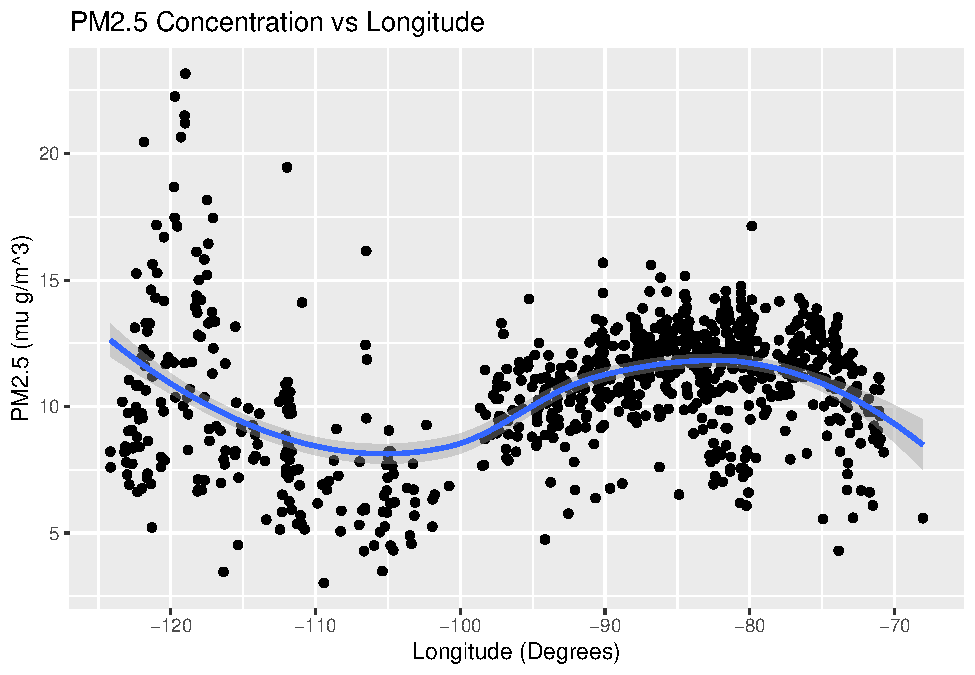
\includegraphics{Draft_files/figure-latex/ExploratoryAnalysis-1.pdf}

\begin{Shaded}
\begin{Highlighting}[]
\NormalTok{origin }\SpecialCharTok{\%\textgreater{}\%} \FunctionTok{ggplot}\NormalTok{(}\FunctionTok{aes}\NormalTok{(}\AttributeTok{x=}\NormalTok{lat, }\AttributeTok{y=}\NormalTok{value)) }\SpecialCharTok{+} 
  \FunctionTok{geom\_point}\NormalTok{() }\SpecialCharTok{+} \FunctionTok{geom\_smooth}\NormalTok{() }\SpecialCharTok{+} 
  \FunctionTok{labs}\NormalTok{(}\AttributeTok{title=}\StringTok{"PM2.5 Concentration vs Latitude"}\NormalTok{, }\AttributeTok{x=}\StringTok{"Latitude (Degrees)"}\NormalTok{, }\AttributeTok{y=}\StringTok{"PM2.5 (mu g/m\^{}3)"}\NormalTok{)}
\end{Highlighting}
\end{Shaded}

\begin{verbatim}
## `geom_smooth()` using method = 'loess' and formula = 'y ~ x'
\end{verbatim}

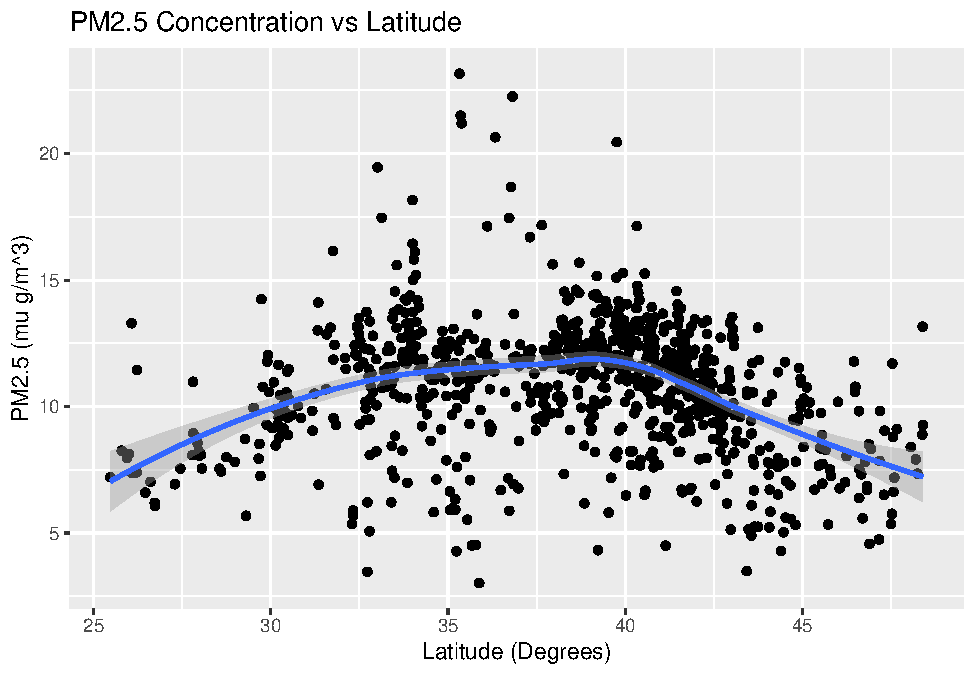
\includegraphics{Draft_files/figure-latex/ExploratoryAnalysis-2.pdf}

\hypertarget{results}{%
\subsection{Results}\label{results}}

\hypertarget{predictorfeature-extraction}{%
\subsubsection{Predictor/Feature
Extraction}\label{predictorfeature-extraction}}

We used the random forest algorithm (RF) to determine which variables
would be the best predictors for our model since RF is good at using
variance to determine which features would be most influential for a
model's predictive performance. In other words, the more variability
there is in a dataset, the better RF performs at predicting which
variables contribute to the outcome by averaging the results of all
trees at the end and this averaging reduces the model's variance. Since
our dataset has a wide variety of predictors ranging from education
attainment levels to poverty levels in a given monitor region to
emission data, RF would be good at reducing the variance in our dataset.
For a given feature, the lower its impurity levels are, the more
important that feature is. As a result, we got an ordered list of
important variables and took the top 5 as input for the training set for
our models. The top 5 important predictors were `CMAQ', `lat',
`county\_area', `lon', and `aod'. We will use these features to predict
`value' proceeding onward. This website was used:
\href{https://towardsdatascience.com/feature-selection-using-random-forest-26d7b747597f}{TowardDataScience}.

\begin{Shaded}
\begin{Highlighting}[]
\CommentTok{\# Use Random Forest for variable selection}
\NormalTok{rfmodel }\OtherTok{=} \FunctionTok{randomForest}\NormalTok{(value}\SpecialCharTok{\textasciitilde{}}\NormalTok{., }\AttributeTok{data=}\NormalTok{train[,}\DecValTok{2}\SpecialCharTok{:}\DecValTok{50}\NormalTok{])}
\NormalTok{import}\OtherTok{=}\FunctionTok{as.data.frame}\NormalTok{(randomForest}\SpecialCharTok{::}\FunctionTok{importance}\NormalTok{(rfmodel)) }\SpecialCharTok{|\textgreater{}} \FunctionTok{arrange}\NormalTok{(}\FunctionTok{desc}\NormalTok{(IncNodePurity))}
\NormalTok{import}\OtherTok{=}\NormalTok{tibble}\SpecialCharTok{::}\FunctionTok{rownames\_to\_column}\NormalTok{(import, }\StringTok{\textquotesingle{}variables\textquotesingle{}}\NormalTok{)}

\CommentTok{\# take top 5 important variables}
\NormalTok{import5 }\OtherTok{=}\NormalTok{ import[}\DecValTok{1}\SpecialCharTok{:}\DecValTok{5}\NormalTok{,]}
\end{Highlighting}
\end{Shaded}

\hypertarget{models}{%
\subsubsection{Models}\label{models}}

\hypertarget{linear-regression}{%
\subsubsection{1. Linear Regression}\label{linear-regression}}

For linear regression (LR), the unscaled training set was used since
variance does not affect the prediction performance of this model. Step
Akaike Information Criteria (AIC) was used to simplify feature amount
without impacting the model's performance. Features are dropped as the
AIC score decreases and feature dropping stops once the AIC score
increases. `CMAQ'and 'aod' were determined to be the most important
features, and these predictors were used in the recipe. Then, the model
was fitted. Using the summary function, we found the LR model had a RMSE
of 2.27 performance. After 10-fold cross validation, the RMSE score was
over 1, indicating that this model's prediction performance is not good.

\begin{Shaded}
\begin{Highlighting}[]
\FunctionTok{set.seed}\NormalTok{(}\DecValTok{123}\NormalTok{)}
\CommentTok{\# Fit model and get summary}
\NormalTok{fit\_lm }\OtherTok{=} \FunctionTok{lm}\NormalTok{(value }\SpecialCharTok{\textasciitilde{}}\NormalTok{ CMAQ}\SpecialCharTok{+}\NormalTok{lat}\SpecialCharTok{+}\NormalTok{county\_area}\SpecialCharTok{+}\NormalTok{lon}\SpecialCharTok{+}\NormalTok{aod, }\AttributeTok{data=}\NormalTok{train)}
\NormalTok{step }\OtherTok{\textless{}{-}} \FunctionTok{stepAIC}\NormalTok{(fit\_lm, }\AttributeTok{direction=}\StringTok{"backward"}\NormalTok{, }\AttributeTok{trace=}\ConstantTok{TRUE}\NormalTok{)}
\end{Highlighting}
\end{Shaded}

\begin{verbatim}
## Start:  AIC=1166.85
## value ~ CMAQ + lat + county_area + lon + aod
## 
##               Df Sum of Sq    RSS    AIC
## - lon          1      0.12 3644.2 1164.9
## - lat          1      2.50 3646.6 1165.3
## - county_area  1      2.81 3646.9 1165.4
## <none>                     3644.1 1166.8
## - aod          1    217.29 3861.4 1205.4
## - CMAQ         1    396.56 4040.7 1237.2
## 
## Step:  AIC=1164.87
## value ~ CMAQ + lat + county_area + aod
## 
##               Df Sum of Sq    RSS    AIC
## - lat          1      2.59 3646.8 1163.4
## - county_area  1      3.03 3647.3 1163.5
## <none>                     3644.2 1164.9
## - aod          1    218.47 3862.7 1203.6
## - CMAQ         1    426.81 4071.0 1240.4
## 
## Step:  AIC=1163.37
## value ~ CMAQ + county_area + aod
## 
##               Df Sum of Sq    RSS    AIC
## - county_area  1      2.35 3649.2 1161.8
## <none>                     3646.8 1163.4
## - aod          1    220.86 3867.7 1202.5
## - CMAQ         1    560.41 4207.2 1261.4
## 
## Step:  AIC=1161.82
## value ~ CMAQ + aod
## 
##        Df Sum of Sq    RSS    AIC
## <none>              3649.2 1161.8
## - aod   1    227.72 3876.9 1202.2
## - CMAQ  1    580.05 4229.2 1263.1
\end{verbatim}

\begin{Shaded}
\begin{Highlighting}[]
\CommentTok{\# Keeps cmaq and aod}

\CommentTok{\# Create the recipe for all models}
\NormalTok{rec1 }\OtherTok{\textless{}{-}}\NormalTok{ train }\SpecialCharTok{\%\textgreater{}\%} 
    \FunctionTok{recipe}\NormalTok{(value }\SpecialCharTok{\textasciitilde{}}\NormalTok{ CMAQ}\SpecialCharTok{+}\NormalTok{aod) }

\CommentTok{\# Linear regr. model}
\NormalTok{model1 }\OtherTok{\textless{}{-}} \FunctionTok{linear\_reg}\NormalTok{() }\SpecialCharTok{\%\textgreater{}\%} 
    \FunctionTok{set\_engine}\NormalTok{(}\StringTok{"lm"}\NormalTok{) }\SpecialCharTok{\%\textgreater{}\%} 
    \FunctionTok{set\_mode}\NormalTok{(}\StringTok{"regression"}\NormalTok{)}

\NormalTok{wf1 }\OtherTok{\textless{}{-}} \FunctionTok{workflow}\NormalTok{() }\SpecialCharTok{\%\textgreater{}\%} 
    \FunctionTok{add\_recipe}\NormalTok{(rec1) }\SpecialCharTok{\%\textgreater{}\%} 
    \FunctionTok{add\_model}\NormalTok{(model1)}
\CommentTok{\# wf1}

\NormalTok{res1 }\OtherTok{\textless{}{-}}\NormalTok{ wf1 }\SpecialCharTok{|\textgreater{}}\NormalTok{ parsnip}\SpecialCharTok{::}\FunctionTok{fit}\NormalTok{(}\AttributeTok{data =}\NormalTok{ train)}

\CommentTok{\# Check performance of linear regression model on the training data}
\NormalTok{res1 }\SpecialCharTok{\%\textgreater{}\%} 
    \FunctionTok{extract\_fit\_engine}\NormalTok{() }\SpecialCharTok{\%\textgreater{}\%} 
    \FunctionTok{summary}\NormalTok{()}
\end{Highlighting}
\end{Shaded}

\begin{verbatim}
## 
## Call:
## stats::lm(formula = ..y ~ ., data = data)
## 
## Residuals:
##     Min      1Q  Median      3Q     Max 
## -6.4165 -1.1913 -0.0098  1.1486 12.8274 
## 
## Coefficients:
##             Estimate Std. Error t value Pr(>|t|)    
## (Intercept) 6.735167   0.284723  23.655  < 2e-16 ***
## CMAQ        0.327107   0.031077  10.526  < 2e-16 ***
## aod         0.030750   0.004663   6.595 8.41e-11 ***
## ---
## Signif. codes:  0 '***' 0.001 '**' 0.01 '*' 0.05 '.' 0.1 ' ' 1
## 
## Residual standard error: 2.288 on 697 degrees of freedom
## Multiple R-squared:  0.2458, Adjusted R-squared:  0.2437 
## F-statistic: 113.6 on 2 and 697 DF,  p-value: < 2.2e-16
\end{verbatim}

\begin{Shaded}
\begin{Highlighting}[]
\CommentTok{\# Check linear regression model performance using cross{-}validation}
\NormalTok{folds1 }\OtherTok{\textless{}{-}} \FunctionTok{vfold\_cv}\NormalTok{(train, }\AttributeTok{v =} \DecValTok{10}\NormalTok{)}
\CommentTok{\# folds1}
\NormalTok{res1 }\OtherTok{\textless{}{-}} \FunctionTok{fit\_resamples}\NormalTok{(wf1, }\AttributeTok{resamples =}\NormalTok{ folds1)}
\NormalTok{res1 }\SpecialCharTok{\%\textgreater{}\%} 
    \FunctionTok{collect\_metrics}\NormalTok{()}
\end{Highlighting}
\end{Shaded}

\begin{verbatim}
## # A tibble: 2 x 6
##   .metric .estimator  mean     n std_err .config             
##   <chr>   <chr>      <dbl> <int>   <dbl> <chr>               
## 1 rmse    standard   2.27     10  0.118  Preprocessor1_Model1
## 2 rsq     standard   0.249    10  0.0216 Preprocessor1_Model1
\end{verbatim}

\hypertarget{k-nearest-neighbors}{%
\subsubsection{2. K-Nearest Neighbors}\label{k-nearest-neighbors}}

The K-Nearest Neighbors (KNN) model finds the predicted `value' by
taking the average `value' of its k neighbors. We first found the ideal
number of k neighbors. This was determined by finding the square root of
the number of observations, which was rounded to be 26. We fit the model
on the training set data and checked its performance using two methods:
the first was fitting the model to extracting the MAE and MSE and the
second was 10-fold cross validation. RMSE is the square root of MSE and
we were able to confirm its value in the cross-validation by comparing
it to the square root of MSE attained from the first method. We found
that after 10-fold cross validation, the RMSE was 1.84. This indicates
that the model does not predict well since the amount of error is
greater than 1.

\begin{Shaded}
\begin{Highlighting}[]
\CommentTok{\# kNN uses scaled data called train\_knn}
\FunctionTok{set.seed}\NormalTok{(}\DecValTok{123}\NormalTok{)}
\CommentTok{\# Find ideal k neighbors}
\FunctionTok{sqrt}\NormalTok{(}\FunctionTok{nrow}\NormalTok{(train))}
\end{Highlighting}
\end{Shaded}

\begin{verbatim}
## [1] 26.45751
\end{verbatim}

\begin{Shaded}
\begin{Highlighting}[]
\CommentTok{\# Create recipe}
\NormalTok{rec2 }\OtherTok{=}\NormalTok{ train\_knn }\SpecialCharTok{|\textgreater{}} \FunctionTok{recipe}\NormalTok{(value }\SpecialCharTok{\textasciitilde{}}\NormalTok{ CMAQ}\SpecialCharTok{+}\NormalTok{lat}\SpecialCharTok{+}\NormalTok{county\_area}\SpecialCharTok{+}\NormalTok{lon}\SpecialCharTok{+}\NormalTok{aod)}

\CommentTok{\# Create kNN model}
\NormalTok{model2 }\OtherTok{\textless{}{-}} \FunctionTok{nearest\_neighbor}\NormalTok{(}\AttributeTok{neighbors =} \DecValTok{26}\NormalTok{) }\SpecialCharTok{\%\textgreater{}\%} 
    \FunctionTok{set\_engine}\NormalTok{(}\StringTok{"kknn"}\NormalTok{) }\SpecialCharTok{\%\textgreater{}\%} 
    \FunctionTok{set\_mode}\NormalTok{(}\StringTok{"regression"}\NormalTok{)}

\CommentTok{\# Create workflow}
\NormalTok{  wf2 }\OtherTok{\textless{}{-}} \FunctionTok{workflow}\NormalTok{() }\SpecialCharTok{\%\textgreater{}\%} 
    \FunctionTok{add\_recipe}\NormalTok{(rec2) }\SpecialCharTok{\%\textgreater{}\%} 
    \FunctionTok{add\_model}\NormalTok{(model2)}

\CommentTok{\# Fit the model on the training dataset using the \textasciigrave{}fit()\textasciigrave{} function}
\NormalTok{res2 }\OtherTok{\textless{}{-}}\NormalTok{ parsnip}\SpecialCharTok{::}\FunctionTok{fit}\NormalTok{(wf2, }\AttributeTok{data =}\NormalTok{ train\_knn)}
\end{Highlighting}
\end{Shaded}

\begin{verbatim}
## Warning: package 'kknn' was built under R version 4.2.3
\end{verbatim}

\begin{verbatim}
## 
## Attaching package: 'kknn'
\end{verbatim}

\begin{verbatim}
## The following object is masked from 'package:caret':
## 
##     contr.dummy
\end{verbatim}

\begin{Shaded}
\begin{Highlighting}[]
\CommentTok{\# Check performance on the complete training data}
\NormalTok{res2 }\SpecialCharTok{\%\textgreater{}\%} 
    \FunctionTok{extract\_fit\_engine}\NormalTok{() }\SpecialCharTok{\%\textgreater{}\%} 
    \FunctionTok{summary}\NormalTok{()}
\end{Highlighting}
\end{Shaded}

\begin{verbatim}
## 
## Call:
## kknn::train.kknn(formula = ..y ~ ., data = data, ks = min_rows(26,     data, 5))
## 
## Type of response variable: continuous
## minimal mean absolute error: 1.257437
## Minimal mean squared error: 3.327239
## Best kernel: optimal
## Best k: 26
\end{verbatim}

\begin{Shaded}
\begin{Highlighting}[]
\CommentTok{\# Check performance using cross{-}validation}
\NormalTok{folds2 }\OtherTok{\textless{}{-}} \FunctionTok{vfold\_cv}\NormalTok{(train\_knn, }\AttributeTok{v =} \DecValTok{10}\NormalTok{)}
\CommentTok{\# folds}
\NormalTok{res2 }\OtherTok{\textless{}{-}} \FunctionTok{fit\_resamples}\NormalTok{(wf2, }\AttributeTok{resamples =}\NormalTok{ folds2) }\CommentTok{\# ERROR Assigned data \textasciigrave{}orig\_rows\textasciigrave{} must be compatible with existing data.}
\NormalTok{res2 }\SpecialCharTok{\%\textgreater{}\%} 
    \FunctionTok{collect\_metrics}\NormalTok{()}
\end{Highlighting}
\end{Shaded}

\begin{verbatim}
## # A tibble: 2 x 6
##   .metric .estimator  mean     n std_err .config             
##   <chr>   <chr>      <dbl> <int>   <dbl> <chr>               
## 1 rmse    standard   1.84     10  0.0842 Preprocessor1_Model1
## 2 rsq     standard   0.514    10  0.0381 Preprocessor1_Model1
\end{verbatim}

\hypertarget{extreme-gradient-boost-regression}{%
\subsubsection{3. Extreme Gradient Boost
Regression}\label{extreme-gradient-boost-regression}}

The Extreme Gradient Boosting (XGB) model performs by training weak
learners, models that have low prediction accuracy, sequentially to
become a single strong learner, a model that has strong prediction
accuracy. We preprocess the training set to make the predictive modeling
process more accurate and smoother by prepping (estimates the quantities
for `train\_scaled') and baking (assigns prepped data to an object) the
data. The aforementioned top 5 predictors were used in this `rec3'.
Moreover, the categorical variables were factored and features with no
variance were removed before this data was baked. Then, this processed
data is assigned to `folds3' and resampled on 5 subsets of the training
set. Using `fold3', we tune the hyperparameters to make the modeling
process more efficient and perform grid specification to determine which
hyperparameter values have high prediction accuracy (i.e.~low prediction
error). Next, we isolated the best hyperparameter values, so they can be
used for the final boosting model. Lastly, we fitted the model and
evaluated its prediction performance. Its RMSE score was 0.23,
indicating that XG Boost is an adequate model. This website was used:
\href{https://www.r-bloggers.com/2020/05/using-xgboost-with-tidymodels/}{RBloggers}

\begin{Shaded}
\begin{Highlighting}[]
\FunctionTok{set.seed}\NormalTok{(}\DecValTok{123}\NormalTok{)}
\CommentTok{\# Preprocessing recipe}
\NormalTok{rec3 }\OtherTok{\textless{}{-}} 
\NormalTok{  recipes}\SpecialCharTok{::}\FunctionTok{recipe}\NormalTok{(value }\SpecialCharTok{\textasciitilde{}}\NormalTok{ CMAQ}\SpecialCharTok{+}\NormalTok{lat}\SpecialCharTok{+}\NormalTok{county\_area}\SpecialCharTok{+}\NormalTok{lon}\SpecialCharTok{+}\NormalTok{aod, }\AttributeTok{data =} \FunctionTok{training}\NormalTok{(dat\_split)) }\SpecialCharTok{\%\textgreater{}\%}
  \CommentTok{\# Convert categorical variables to factors}
\NormalTok{  recipes}\SpecialCharTok{::}\FunctionTok{step\_string2factor}\NormalTok{(}\FunctionTok{all\_nominal}\NormalTok{()) }\SpecialCharTok{\%\textgreater{}\%}
  \CommentTok{\# Combine low frequency factor levels}
\NormalTok{  recipes}\SpecialCharTok{::}\FunctionTok{step\_other}\NormalTok{(}\FunctionTok{all\_nominal}\NormalTok{(), }\AttributeTok{threshold =} \FloatTok{0.01}\NormalTok{) }\SpecialCharTok{\%\textgreater{}\%}
  \CommentTok{\# Remove no variance predictors which provide no predictive information }
\NormalTok{  recipes}\SpecialCharTok{::}\FunctionTok{step\_nzv}\NormalTok{(}\FunctionTok{all\_nominal}\NormalTok{()) }\SpecialCharTok{\%\textgreater{}\%}
  \FunctionTok{prep}\NormalTok{()}

\NormalTok{folds3 }\OtherTok{\textless{}{-}}\NormalTok{ recipes}\SpecialCharTok{::}\FunctionTok{bake}\NormalTok{(rec3, }\AttributeTok{new\_data =} \FunctionTok{training}\NormalTok{(dat\_split)) }\SpecialCharTok{\%\textgreater{}\%}  
\NormalTok{  rsample}\SpecialCharTok{::}\FunctionTok{vfold\_cv}\NormalTok{(}\AttributeTok{v =} \DecValTok{5}\NormalTok{)}

\CommentTok{\# XGBoost model specification}
\NormalTok{xgboost\_model }\OtherTok{\textless{}{-}}\NormalTok{ parsnip}\SpecialCharTok{::}\FunctionTok{boost\_tree}\NormalTok{(}\AttributeTok{mode =} \StringTok{"regression"}\NormalTok{, }\AttributeTok{trees =} \DecValTok{1000}\NormalTok{, }\AttributeTok{min\_n =} \FunctionTok{tune}\NormalTok{(),}
  \AttributeTok{tree\_depth =} \FunctionTok{tune}\NormalTok{(), }\AttributeTok{learn\_rate =} \FunctionTok{tune}\NormalTok{(), }\AttributeTok{loss\_reduction =} \FunctionTok{tune}\NormalTok{()) }\SpecialCharTok{\%\textgreater{}\%}
  \FunctionTok{set\_engine}\NormalTok{(}\StringTok{"xgboost"}\NormalTok{, }\AttributeTok{objective =} \StringTok{"reg:squarederror"}\NormalTok{)}

\CommentTok{\# Grid specification}
\NormalTok{xgboost\_params }\OtherTok{\textless{}{-}}\NormalTok{ dials}\SpecialCharTok{::}\FunctionTok{parameters}\NormalTok{(}\FunctionTok{min\_n}\NormalTok{(), }\FunctionTok{tree\_depth}\NormalTok{(), }\FunctionTok{learn\_rate}\NormalTok{(), }\FunctionTok{loss\_reduction}\NormalTok{())}

\NormalTok{xgboost\_grid }\OtherTok{\textless{}{-}}\NormalTok{ dials}\SpecialCharTok{::}\FunctionTok{grid\_max\_entropy}\NormalTok{(xgboost\_params, }\AttributeTok{size =} \DecValTok{60}\NormalTok{)}

\CommentTok{\# head(xgboost\_grid)}

\NormalTok{xgboost\_wf }\OtherTok{\textless{}{-}}\NormalTok{ workflows}\SpecialCharTok{::}\FunctionTok{workflow}\NormalTok{() }\SpecialCharTok{\%\textgreater{}\%}
  \FunctionTok{add\_model}\NormalTok{(xgboost\_model) }\SpecialCharTok{\%\textgreater{}\%} 
  \FunctionTok{add\_formula}\NormalTok{(value }\SpecialCharTok{\textasciitilde{}}\NormalTok{ CMAQ}\SpecialCharTok{+}\NormalTok{lat}\SpecialCharTok{+}\NormalTok{county\_area}\SpecialCharTok{+}\NormalTok{lon}\SpecialCharTok{+}\NormalTok{aod)}

\CommentTok{\# Hyperparameter tuning}
\CommentTok{\# Takes a long time to run, 5{-}8 min}
\NormalTok{xgboost\_tuned }\OtherTok{\textless{}{-}}\NormalTok{ tune}\SpecialCharTok{::}\FunctionTok{tune\_grid}\NormalTok{(}\AttributeTok{object =}\NormalTok{ xgboost\_wf, }\AttributeTok{resamples =}\NormalTok{ folds3,}
  \AttributeTok{grid =}\NormalTok{ xgboost\_grid, }\AttributeTok{metrics =}\NormalTok{ yardstick}\SpecialCharTok{::}\FunctionTok{metric\_set}\NormalTok{(rmse, rsq),}
  \AttributeTok{control =}\NormalTok{ tune}\SpecialCharTok{::}\FunctionTok{control\_grid}\NormalTok{(}\AttributeTok{verbose =} \ConstantTok{TRUE}\NormalTok{))}
\end{Highlighting}
\end{Shaded}

\begin{verbatim}
## i Fold1: preprocessor 1/1
\end{verbatim}

\begin{verbatim}
## v Fold1: preprocessor 1/1
\end{verbatim}

\begin{verbatim}
## i Fold1: preprocessor 1/1, model 1/60
\end{verbatim}

\begin{verbatim}
## v Fold1: preprocessor 1/1, model 1/60
\end{verbatim}

\begin{verbatim}
## i Fold1: preprocessor 1/1, model 1/60 (extracts)
\end{verbatim}

\begin{verbatim}
## i Fold1: preprocessor 1/1, model 1/60 (predictions)
\end{verbatim}

\begin{verbatim}
## i Fold1: preprocessor 1/1, model 2/60
\end{verbatim}

\begin{verbatim}
## v Fold1: preprocessor 1/1, model 2/60
\end{verbatim}

\begin{verbatim}
## i Fold1: preprocessor 1/1, model 2/60 (extracts)
\end{verbatim}

\begin{verbatim}
## i Fold1: preprocessor 1/1, model 2/60 (predictions)
\end{verbatim}

\begin{verbatim}
## i Fold1: preprocessor 1/1, model 3/60
\end{verbatim}

\begin{verbatim}
## v Fold1: preprocessor 1/1, model 3/60
\end{verbatim}

\begin{verbatim}
## i Fold1: preprocessor 1/1, model 3/60 (extracts)
\end{verbatim}

\begin{verbatim}
## i Fold1: preprocessor 1/1, model 3/60 (predictions)
\end{verbatim}

\begin{verbatim}
## i Fold1: preprocessor 1/1, model 4/60
\end{verbatim}

\begin{verbatim}
## v Fold1: preprocessor 1/1, model 4/60
\end{verbatim}

\begin{verbatim}
## i Fold1: preprocessor 1/1, model 4/60 (extracts)
\end{verbatim}

\begin{verbatim}
## i Fold1: preprocessor 1/1, model 4/60 (predictions)
\end{verbatim}

\begin{verbatim}
## i Fold1: preprocessor 1/1, model 5/60
\end{verbatim}

\begin{verbatim}
## v Fold1: preprocessor 1/1, model 5/60
\end{verbatim}

\begin{verbatim}
## i Fold1: preprocessor 1/1, model 5/60 (extracts)
\end{verbatim}

\begin{verbatim}
## i Fold1: preprocessor 1/1, model 5/60 (predictions)
\end{verbatim}

\begin{verbatim}
## i Fold1: preprocessor 1/1, model 6/60
\end{verbatim}

\begin{verbatim}
## v Fold1: preprocessor 1/1, model 6/60
\end{verbatim}

\begin{verbatim}
## i Fold1: preprocessor 1/1, model 6/60 (extracts)
\end{verbatim}

\begin{verbatim}
## i Fold1: preprocessor 1/1, model 6/60 (predictions)
\end{verbatim}

\begin{verbatim}
## i Fold1: preprocessor 1/1, model 7/60
\end{verbatim}

\begin{verbatim}
## v Fold1: preprocessor 1/1, model 7/60
\end{verbatim}

\begin{verbatim}
## i Fold1: preprocessor 1/1, model 7/60 (extracts)
\end{verbatim}

\begin{verbatim}
## i Fold1: preprocessor 1/1, model 7/60 (predictions)
\end{verbatim}

\begin{verbatim}
## i Fold1: preprocessor 1/1, model 8/60
\end{verbatim}

\begin{verbatim}
## v Fold1: preprocessor 1/1, model 8/60
\end{verbatim}

\begin{verbatim}
## i Fold1: preprocessor 1/1, model 8/60 (extracts)
\end{verbatim}

\begin{verbatim}
## i Fold1: preprocessor 1/1, model 8/60 (predictions)
\end{verbatim}

\begin{verbatim}
## i Fold1: preprocessor 1/1, model 9/60
\end{verbatim}

\begin{verbatim}
## v Fold1: preprocessor 1/1, model 9/60
\end{verbatim}

\begin{verbatim}
## i Fold1: preprocessor 1/1, model 9/60 (extracts)
\end{verbatim}

\begin{verbatim}
## i Fold1: preprocessor 1/1, model 9/60 (predictions)
\end{verbatim}

\begin{verbatim}
## i Fold1: preprocessor 1/1, model 10/60
\end{verbatim}

\begin{verbatim}
## v Fold1: preprocessor 1/1, model 10/60
\end{verbatim}

\begin{verbatim}
## i Fold1: preprocessor 1/1, model 10/60 (extracts)
\end{verbatim}

\begin{verbatim}
## i Fold1: preprocessor 1/1, model 10/60 (predictions)
\end{verbatim}

\begin{verbatim}
## i Fold1: preprocessor 1/1, model 11/60
\end{verbatim}

\begin{verbatim}
## v Fold1: preprocessor 1/1, model 11/60
\end{verbatim}

\begin{verbatim}
## i Fold1: preprocessor 1/1, model 11/60 (extracts)
\end{verbatim}

\begin{verbatim}
## i Fold1: preprocessor 1/1, model 11/60 (predictions)
\end{verbatim}

\begin{verbatim}
## i Fold1: preprocessor 1/1, model 12/60
\end{verbatim}

\begin{verbatim}
## v Fold1: preprocessor 1/1, model 12/60
\end{verbatim}

\begin{verbatim}
## i Fold1: preprocessor 1/1, model 12/60 (extracts)
\end{verbatim}

\begin{verbatim}
## i Fold1: preprocessor 1/1, model 12/60 (predictions)
\end{verbatim}

\begin{verbatim}
## i Fold1: preprocessor 1/1, model 13/60
\end{verbatim}

\begin{verbatim}
## v Fold1: preprocessor 1/1, model 13/60
\end{verbatim}

\begin{verbatim}
## i Fold1: preprocessor 1/1, model 13/60 (extracts)
\end{verbatim}

\begin{verbatim}
## i Fold1: preprocessor 1/1, model 13/60 (predictions)
\end{verbatim}

\begin{verbatim}
## i Fold1: preprocessor 1/1, model 14/60
\end{verbatim}

\begin{verbatim}
## v Fold1: preprocessor 1/1, model 14/60
\end{verbatim}

\begin{verbatim}
## i Fold1: preprocessor 1/1, model 14/60 (extracts)
\end{verbatim}

\begin{verbatim}
## i Fold1: preprocessor 1/1, model 14/60 (predictions)
\end{verbatim}

\begin{verbatim}
## i Fold1: preprocessor 1/1, model 15/60
\end{verbatim}

\begin{verbatim}
## v Fold1: preprocessor 1/1, model 15/60
\end{verbatim}

\begin{verbatim}
## i Fold1: preprocessor 1/1, model 15/60 (extracts)
\end{verbatim}

\begin{verbatim}
## i Fold1: preprocessor 1/1, model 15/60 (predictions)
\end{verbatim}

\begin{verbatim}
## i Fold1: preprocessor 1/1, model 16/60
\end{verbatim}

\begin{verbatim}
## v Fold1: preprocessor 1/1, model 16/60
\end{verbatim}

\begin{verbatim}
## i Fold1: preprocessor 1/1, model 16/60 (extracts)
\end{verbatim}

\begin{verbatim}
## i Fold1: preprocessor 1/1, model 16/60 (predictions)
\end{verbatim}

\begin{verbatim}
## i Fold1: preprocessor 1/1, model 17/60
\end{verbatim}

\begin{verbatim}
## v Fold1: preprocessor 1/1, model 17/60
\end{verbatim}

\begin{verbatim}
## i Fold1: preprocessor 1/1, model 17/60 (extracts)
\end{verbatim}

\begin{verbatim}
## i Fold1: preprocessor 1/1, model 17/60 (predictions)
\end{verbatim}

\begin{verbatim}
## i Fold1: preprocessor 1/1, model 18/60
\end{verbatim}

\begin{verbatim}
## v Fold1: preprocessor 1/1, model 18/60
\end{verbatim}

\begin{verbatim}
## i Fold1: preprocessor 1/1, model 18/60 (extracts)
\end{verbatim}

\begin{verbatim}
## i Fold1: preprocessor 1/1, model 18/60 (predictions)
\end{verbatim}

\begin{verbatim}
## i Fold1: preprocessor 1/1, model 19/60
\end{verbatim}

\begin{verbatim}
## v Fold1: preprocessor 1/1, model 19/60
\end{verbatim}

\begin{verbatim}
## i Fold1: preprocessor 1/1, model 19/60 (extracts)
\end{verbatim}

\begin{verbatim}
## i Fold1: preprocessor 1/1, model 19/60 (predictions)
\end{verbatim}

\begin{verbatim}
## i Fold1: preprocessor 1/1, model 20/60
\end{verbatim}

\begin{verbatim}
## v Fold1: preprocessor 1/1, model 20/60
\end{verbatim}

\begin{verbatim}
## i Fold1: preprocessor 1/1, model 20/60 (extracts)
\end{verbatim}

\begin{verbatim}
## i Fold1: preprocessor 1/1, model 20/60 (predictions)
\end{verbatim}

\begin{verbatim}
## i Fold1: preprocessor 1/1, model 21/60
\end{verbatim}

\begin{verbatim}
## v Fold1: preprocessor 1/1, model 21/60
\end{verbatim}

\begin{verbatim}
## i Fold1: preprocessor 1/1, model 21/60 (extracts)
\end{verbatim}

\begin{verbatim}
## i Fold1: preprocessor 1/1, model 21/60 (predictions)
\end{verbatim}

\begin{verbatim}
## i Fold1: preprocessor 1/1, model 22/60
\end{verbatim}

\begin{verbatim}
## v Fold1: preprocessor 1/1, model 22/60
\end{verbatim}

\begin{verbatim}
## i Fold1: preprocessor 1/1, model 22/60 (extracts)
\end{verbatim}

\begin{verbatim}
## i Fold1: preprocessor 1/1, model 22/60 (predictions)
\end{verbatim}

\begin{verbatim}
## i Fold1: preprocessor 1/1, model 23/60
\end{verbatim}

\begin{verbatim}
## v Fold1: preprocessor 1/1, model 23/60
\end{verbatim}

\begin{verbatim}
## i Fold1: preprocessor 1/1, model 23/60 (extracts)
\end{verbatim}

\begin{verbatim}
## i Fold1: preprocessor 1/1, model 23/60 (predictions)
\end{verbatim}

\begin{verbatim}
## i Fold1: preprocessor 1/1, model 24/60
\end{verbatim}

\begin{verbatim}
## v Fold1: preprocessor 1/1, model 24/60
\end{verbatim}

\begin{verbatim}
## i Fold1: preprocessor 1/1, model 24/60 (extracts)
\end{verbatim}

\begin{verbatim}
## i Fold1: preprocessor 1/1, model 24/60 (predictions)
\end{verbatim}

\begin{verbatim}
## i Fold1: preprocessor 1/1, model 25/60
\end{verbatim}

\begin{verbatim}
## v Fold1: preprocessor 1/1, model 25/60
\end{verbatim}

\begin{verbatim}
## i Fold1: preprocessor 1/1, model 25/60 (extracts)
\end{verbatim}

\begin{verbatim}
## i Fold1: preprocessor 1/1, model 25/60 (predictions)
\end{verbatim}

\begin{verbatim}
## i Fold1: preprocessor 1/1, model 26/60
\end{verbatim}

\begin{verbatim}
## v Fold1: preprocessor 1/1, model 26/60
\end{verbatim}

\begin{verbatim}
## i Fold1: preprocessor 1/1, model 26/60 (extracts)
\end{verbatim}

\begin{verbatim}
## i Fold1: preprocessor 1/1, model 26/60 (predictions)
\end{verbatim}

\begin{verbatim}
## i Fold1: preprocessor 1/1, model 27/60
\end{verbatim}

\begin{verbatim}
## v Fold1: preprocessor 1/1, model 27/60
\end{verbatim}

\begin{verbatim}
## i Fold1: preprocessor 1/1, model 27/60 (extracts)
\end{verbatim}

\begin{verbatim}
## i Fold1: preprocessor 1/1, model 27/60 (predictions)
\end{verbatim}

\begin{verbatim}
## i Fold1: preprocessor 1/1, model 28/60
\end{verbatim}

\begin{verbatim}
## v Fold1: preprocessor 1/1, model 28/60
\end{verbatim}

\begin{verbatim}
## i Fold1: preprocessor 1/1, model 28/60 (extracts)
\end{verbatim}

\begin{verbatim}
## i Fold1: preprocessor 1/1, model 28/60 (predictions)
\end{verbatim}

\begin{verbatim}
## i Fold1: preprocessor 1/1, model 29/60
\end{verbatim}

\begin{verbatim}
## v Fold1: preprocessor 1/1, model 29/60
\end{verbatim}

\begin{verbatim}
## i Fold1: preprocessor 1/1, model 29/60 (extracts)
\end{verbatim}

\begin{verbatim}
## i Fold1: preprocessor 1/1, model 29/60 (predictions)
\end{verbatim}

\begin{verbatim}
## i Fold1: preprocessor 1/1, model 30/60
\end{verbatim}

\begin{verbatim}
## v Fold1: preprocessor 1/1, model 30/60
\end{verbatim}

\begin{verbatim}
## i Fold1: preprocessor 1/1, model 30/60 (extracts)
\end{verbatim}

\begin{verbatim}
## i Fold1: preprocessor 1/1, model 30/60 (predictions)
\end{verbatim}

\begin{verbatim}
## i Fold1: preprocessor 1/1, model 31/60
\end{verbatim}

\begin{verbatim}
## v Fold1: preprocessor 1/1, model 31/60
\end{verbatim}

\begin{verbatim}
## i Fold1: preprocessor 1/1, model 31/60 (extracts)
\end{verbatim}

\begin{verbatim}
## i Fold1: preprocessor 1/1, model 31/60 (predictions)
\end{verbatim}

\begin{verbatim}
## i Fold1: preprocessor 1/1, model 32/60
\end{verbatim}

\begin{verbatim}
## v Fold1: preprocessor 1/1, model 32/60
\end{verbatim}

\begin{verbatim}
## i Fold1: preprocessor 1/1, model 32/60 (extracts)
\end{verbatim}

\begin{verbatim}
## i Fold1: preprocessor 1/1, model 32/60 (predictions)
\end{verbatim}

\begin{verbatim}
## i Fold1: preprocessor 1/1, model 33/60
\end{verbatim}

\begin{verbatim}
## v Fold1: preprocessor 1/1, model 33/60
\end{verbatim}

\begin{verbatim}
## i Fold1: preprocessor 1/1, model 33/60 (extracts)
\end{verbatim}

\begin{verbatim}
## i Fold1: preprocessor 1/1, model 33/60 (predictions)
\end{verbatim}

\begin{verbatim}
## i Fold1: preprocessor 1/1, model 34/60
\end{verbatim}

\begin{verbatim}
## v Fold1: preprocessor 1/1, model 34/60
\end{verbatim}

\begin{verbatim}
## i Fold1: preprocessor 1/1, model 34/60 (extracts)
\end{verbatim}

\begin{verbatim}
## i Fold1: preprocessor 1/1, model 34/60 (predictions)
\end{verbatim}

\begin{verbatim}
## i Fold1: preprocessor 1/1, model 35/60
\end{verbatim}

\begin{verbatim}
## v Fold1: preprocessor 1/1, model 35/60
\end{verbatim}

\begin{verbatim}
## i Fold1: preprocessor 1/1, model 35/60 (extracts)
\end{verbatim}

\begin{verbatim}
## i Fold1: preprocessor 1/1, model 35/60 (predictions)
\end{verbatim}

\begin{verbatim}
## i Fold1: preprocessor 1/1, model 36/60
\end{verbatim}

\begin{verbatim}
## v Fold1: preprocessor 1/1, model 36/60
\end{verbatim}

\begin{verbatim}
## i Fold1: preprocessor 1/1, model 36/60 (extracts)
\end{verbatim}

\begin{verbatim}
## i Fold1: preprocessor 1/1, model 36/60 (predictions)
\end{verbatim}

\begin{verbatim}
## i Fold1: preprocessor 1/1, model 37/60
\end{verbatim}

\begin{verbatim}
## v Fold1: preprocessor 1/1, model 37/60
\end{verbatim}

\begin{verbatim}
## i Fold1: preprocessor 1/1, model 37/60 (extracts)
\end{verbatim}

\begin{verbatim}
## i Fold1: preprocessor 1/1, model 37/60 (predictions)
\end{verbatim}

\begin{verbatim}
## i Fold1: preprocessor 1/1, model 38/60
\end{verbatim}

\begin{verbatim}
## v Fold1: preprocessor 1/1, model 38/60
\end{verbatim}

\begin{verbatim}
## i Fold1: preprocessor 1/1, model 38/60 (extracts)
\end{verbatim}

\begin{verbatim}
## i Fold1: preprocessor 1/1, model 38/60 (predictions)
\end{verbatim}

\begin{verbatim}
## i Fold1: preprocessor 1/1, model 39/60
\end{verbatim}

\begin{verbatim}
## v Fold1: preprocessor 1/1, model 39/60
\end{verbatim}

\begin{verbatim}
## i Fold1: preprocessor 1/1, model 39/60 (extracts)
\end{verbatim}

\begin{verbatim}
## i Fold1: preprocessor 1/1, model 39/60 (predictions)
\end{verbatim}

\begin{verbatim}
## i Fold1: preprocessor 1/1, model 40/60
\end{verbatim}

\begin{verbatim}
## v Fold1: preprocessor 1/1, model 40/60
\end{verbatim}

\begin{verbatim}
## i Fold1: preprocessor 1/1, model 40/60 (extracts)
\end{verbatim}

\begin{verbatim}
## i Fold1: preprocessor 1/1, model 40/60 (predictions)
\end{verbatim}

\begin{verbatim}
## i Fold1: preprocessor 1/1, model 41/60
\end{verbatim}

\begin{verbatim}
## v Fold1: preprocessor 1/1, model 41/60
\end{verbatim}

\begin{verbatim}
## i Fold1: preprocessor 1/1, model 41/60 (extracts)
\end{verbatim}

\begin{verbatim}
## i Fold1: preprocessor 1/1, model 41/60 (predictions)
\end{verbatim}

\begin{verbatim}
## i Fold1: preprocessor 1/1, model 42/60
\end{verbatim}

\begin{verbatim}
## v Fold1: preprocessor 1/1, model 42/60
\end{verbatim}

\begin{verbatim}
## i Fold1: preprocessor 1/1, model 42/60 (extracts)
\end{verbatim}

\begin{verbatim}
## i Fold1: preprocessor 1/1, model 42/60 (predictions)
\end{verbatim}

\begin{verbatim}
## i Fold1: preprocessor 1/1, model 43/60
\end{verbatim}

\begin{verbatim}
## v Fold1: preprocessor 1/1, model 43/60
\end{verbatim}

\begin{verbatim}
## i Fold1: preprocessor 1/1, model 43/60 (extracts)
\end{verbatim}

\begin{verbatim}
## i Fold1: preprocessor 1/1, model 43/60 (predictions)
\end{verbatim}

\begin{verbatim}
## i Fold1: preprocessor 1/1, model 44/60
\end{verbatim}

\begin{verbatim}
## v Fold1: preprocessor 1/1, model 44/60
\end{verbatim}

\begin{verbatim}
## i Fold1: preprocessor 1/1, model 44/60 (extracts)
\end{verbatim}

\begin{verbatim}
## i Fold1: preprocessor 1/1, model 44/60 (predictions)
\end{verbatim}

\begin{verbatim}
## i Fold1: preprocessor 1/1, model 45/60
\end{verbatim}

\begin{verbatim}
## v Fold1: preprocessor 1/1, model 45/60
\end{verbatim}

\begin{verbatim}
## i Fold1: preprocessor 1/1, model 45/60 (extracts)
\end{verbatim}

\begin{verbatim}
## i Fold1: preprocessor 1/1, model 45/60 (predictions)
\end{verbatim}

\begin{verbatim}
## i Fold1: preprocessor 1/1, model 46/60
\end{verbatim}

\begin{verbatim}
## v Fold1: preprocessor 1/1, model 46/60
\end{verbatim}

\begin{verbatim}
## i Fold1: preprocessor 1/1, model 46/60 (extracts)
\end{verbatim}

\begin{verbatim}
## i Fold1: preprocessor 1/1, model 46/60 (predictions)
\end{verbatim}

\begin{verbatim}
## i Fold1: preprocessor 1/1, model 47/60
\end{verbatim}

\begin{verbatim}
## v Fold1: preprocessor 1/1, model 47/60
\end{verbatim}

\begin{verbatim}
## i Fold1: preprocessor 1/1, model 47/60 (extracts)
\end{verbatim}

\begin{verbatim}
## i Fold1: preprocessor 1/1, model 47/60 (predictions)
\end{verbatim}

\begin{verbatim}
## i Fold1: preprocessor 1/1, model 48/60
\end{verbatim}

\begin{verbatim}
## v Fold1: preprocessor 1/1, model 48/60
\end{verbatim}

\begin{verbatim}
## i Fold1: preprocessor 1/1, model 48/60 (extracts)
\end{verbatim}

\begin{verbatim}
## i Fold1: preprocessor 1/1, model 48/60 (predictions)
\end{verbatim}

\begin{verbatim}
## i Fold1: preprocessor 1/1, model 49/60
\end{verbatim}

\begin{verbatim}
## v Fold1: preprocessor 1/1, model 49/60
\end{verbatim}

\begin{verbatim}
## i Fold1: preprocessor 1/1, model 49/60 (extracts)
\end{verbatim}

\begin{verbatim}
## i Fold1: preprocessor 1/1, model 49/60 (predictions)
\end{verbatim}

\begin{verbatim}
## i Fold1: preprocessor 1/1, model 50/60
\end{verbatim}

\begin{verbatim}
## v Fold1: preprocessor 1/1, model 50/60
\end{verbatim}

\begin{verbatim}
## i Fold1: preprocessor 1/1, model 50/60 (extracts)
\end{verbatim}

\begin{verbatim}
## i Fold1: preprocessor 1/1, model 50/60 (predictions)
\end{verbatim}

\begin{verbatim}
## i Fold1: preprocessor 1/1, model 51/60
\end{verbatim}

\begin{verbatim}
## v Fold1: preprocessor 1/1, model 51/60
\end{verbatim}

\begin{verbatim}
## i Fold1: preprocessor 1/1, model 51/60 (extracts)
\end{verbatim}

\begin{verbatim}
## i Fold1: preprocessor 1/1, model 51/60 (predictions)
\end{verbatim}

\begin{verbatim}
## i Fold1: preprocessor 1/1, model 52/60
\end{verbatim}

\begin{verbatim}
## v Fold1: preprocessor 1/1, model 52/60
\end{verbatim}

\begin{verbatim}
## i Fold1: preprocessor 1/1, model 52/60 (extracts)
\end{verbatim}

\begin{verbatim}
## i Fold1: preprocessor 1/1, model 52/60 (predictions)
\end{verbatim}

\begin{verbatim}
## i Fold1: preprocessor 1/1, model 53/60
\end{verbatim}

\begin{verbatim}
## v Fold1: preprocessor 1/1, model 53/60
\end{verbatim}

\begin{verbatim}
## i Fold1: preprocessor 1/1, model 53/60 (extracts)
\end{verbatim}

\begin{verbatim}
## i Fold1: preprocessor 1/1, model 53/60 (predictions)
\end{verbatim}

\begin{verbatim}
## i Fold1: preprocessor 1/1, model 54/60
\end{verbatim}

\begin{verbatim}
## v Fold1: preprocessor 1/1, model 54/60
\end{verbatim}

\begin{verbatim}
## i Fold1: preprocessor 1/1, model 54/60 (extracts)
\end{verbatim}

\begin{verbatim}
## i Fold1: preprocessor 1/1, model 54/60 (predictions)
\end{verbatim}

\begin{verbatim}
## i Fold1: preprocessor 1/1, model 55/60
\end{verbatim}

\begin{verbatim}
## v Fold1: preprocessor 1/1, model 55/60
\end{verbatim}

\begin{verbatim}
## i Fold1: preprocessor 1/1, model 55/60 (extracts)
\end{verbatim}

\begin{verbatim}
## i Fold1: preprocessor 1/1, model 55/60 (predictions)
\end{verbatim}

\begin{verbatim}
## i Fold1: preprocessor 1/1, model 56/60
\end{verbatim}

\begin{verbatim}
## v Fold1: preprocessor 1/1, model 56/60
\end{verbatim}

\begin{verbatim}
## i Fold1: preprocessor 1/1, model 56/60 (extracts)
\end{verbatim}

\begin{verbatim}
## i Fold1: preprocessor 1/1, model 56/60 (predictions)
\end{verbatim}

\begin{verbatim}
## i Fold1: preprocessor 1/1, model 57/60
\end{verbatim}

\begin{verbatim}
## v Fold1: preprocessor 1/1, model 57/60
\end{verbatim}

\begin{verbatim}
## i Fold1: preprocessor 1/1, model 57/60 (extracts)
\end{verbatim}

\begin{verbatim}
## i Fold1: preprocessor 1/1, model 57/60 (predictions)
\end{verbatim}

\begin{verbatim}
## i Fold1: preprocessor 1/1, model 58/60
\end{verbatim}

\begin{verbatim}
## v Fold1: preprocessor 1/1, model 58/60
\end{verbatim}

\begin{verbatim}
## i Fold1: preprocessor 1/1, model 58/60 (extracts)
\end{verbatim}

\begin{verbatim}
## i Fold1: preprocessor 1/1, model 58/60 (predictions)
\end{verbatim}

\begin{verbatim}
## i Fold1: preprocessor 1/1, model 59/60
\end{verbatim}

\begin{verbatim}
## v Fold1: preprocessor 1/1, model 59/60
\end{verbatim}

\begin{verbatim}
## i Fold1: preprocessor 1/1, model 59/60 (extracts)
\end{verbatim}

\begin{verbatim}
## i Fold1: preprocessor 1/1, model 59/60 (predictions)
\end{verbatim}

\begin{verbatim}
## i Fold1: preprocessor 1/1, model 60/60
\end{verbatim}

\begin{verbatim}
## v Fold1: preprocessor 1/1, model 60/60
\end{verbatim}

\begin{verbatim}
## i Fold1: preprocessor 1/1, model 60/60 (extracts)
\end{verbatim}

\begin{verbatim}
## i Fold1: preprocessor 1/1, model 60/60 (predictions)
\end{verbatim}

\begin{verbatim}
## ! Fold1: internal:
##   There was 1 warning in `dplyr::summarise()`.
##   i In argument: `.estimate = metric_fn(truth = value, estimate = .pred,...
##     na_rm)`.
##   i In group 1: `min_n = 31`, `tree_depth = 3`, `learn_rate = 4.228428e-...
##     `loss_reduction = 1.230863e-09`.
##   Caused by warning:
##   ! A correlation computation is required, but `estimate` is constant an...
##   i In argument: `.estimate = metric_fn(truth = value, estimate = .pred,...
##     na_rm)`.
##   i In group 1: `min_n = 16`, `tree_depth = 13`, `learn_rate = 8.942791e...
##     `loss_reduction = 2.073912`.
##   Caused by warning:
##   ! A correlation computation is required, but `estimate` is constant an...
##   i In argument: `.estimate = metric_fn(truth = value, estimate = .pred,...
##     na_rm)`.
##   i In group 1: `min_n = 16`, `tree_depth = 5`, `learn_rate = 1.685285e-...
##     `loss_reduction = 9.230063e-10`.
##   Caused by warning:
##   ! A correlation computation is required, but `estimate` is constant an...
##   i In argument: `.estimate = metric_fn(truth = value, estimate = .pred,...
##     na_rm)`.
##   i In group 1: `min_n = 39`, `tree_depth = 14`, `learn_rate = 2.038467e...
##     `loss_reduction = 0.05878203`.
##   Caused by warning:
##   ! A correlation computation is required, but `estimate` is constant an...
##   i In argument: `.estimate = metric_fn(truth = value, estimate = .pred,...
##     na_rm)`.
##   i In group 1: `min_n = 32`, `tree_depth = 6`, `learn_rate = 3.583763e-...
##     `loss_reduction = 0.04223655`.
##   Caused by warning:
##   ! A correlation computation is required, but `estimate` is constant an...
##   i In argument: `.estimate = metric_fn(truth = value, estimate = .pred,...
##     na_rm)`.
##   i In group 1: `min_n = 14`, `tree_depth = 2`, `learn_rate = 1.786541e-...
##     `loss_reduction = 1.142136e-05`.
##   Caused by warning:
##   ! A correlation computation is required, but `estimate` is constant an...
##   i In argument: `.estimate = metric_fn(truth = value, estimate = .pred,...
##     na_rm)`.
##   i In group 1: `min_n = 33`, `tree_depth = 10`, `learn_rate = 5.990585e...
##     `loss_reduction = 3.553207e-07`.
##   Caused by warning:
##   ! A correlation computation is required, but `estimate` is constant an...
##   i In argument: `.estimate = metric_fn(truth = value, estimate = .pred,...
##     na_rm)`.
##   i In group 1: `min_n = 30`, `tree_depth = 14`, `learn_rate = 9.438684e...
##     `loss_reduction = 25.86689`.
##   Caused by warning:
##   ! A correlation computation is required, but `estimate` is constant an...
##   i In argument: `.estimate = metric_fn(truth = value, estimate = .pred,...
##     na_rm)`.
##   i In group 1: `min_n = 13`, `tree_depth = 8`, `learn_rate = 3.959735e-...
##     `loss_reduction = 5.666308e-06`.
##   Caused by warning:
##   ! A correlation computation is required, but `estimate` is constant an...
##   i In argument: `.estimate = metric_fn(truth = value, estimate = .pred,...
##     na_rm)`.
##   i In group 1: `min_n = 5`, `tree_depth = 2`, `learn_rate = 6.002922e-09`,
##     `loss_reduction = 2.467321`.
##   Caused by warning:
##   ! A correlation computation is required, but `estimate` is constant an...
##   i In argument: `.estimate = metric_fn(truth = value, estimate = .pred,...
##     na_rm)`.
##   i In group 1: `min_n = 30`, `tree_depth = 1`, `learn_rate = 1.100178e-...
##     `loss_reduction = 0.0001398712`.
##   Caused by warning:
##   ! A correlation computation is required, but `estimate` is constant an...
##   i In argument: `.estimate = metric_fn(truth = value, estimate = .pred,...
##     na_rm)`.
##   i In group 1: `min_n = 23`, `tree_depth = 10`, `learn_rate = 2.271355e...
##     `loss_reduction = 1.305291e-09`.
##   Caused by warning:
##   ! A correlation computation is required, but `estimate` is constant an...
\end{verbatim}

\begin{verbatim}
## v Fold1: internal
\end{verbatim}

\begin{verbatim}
## i Fold2: preprocessor 1/1
\end{verbatim}

\begin{verbatim}
## v Fold2: preprocessor 1/1
\end{verbatim}

\begin{verbatim}
## i Fold2: preprocessor 1/1, model 1/60
\end{verbatim}

\begin{verbatim}
## v Fold2: preprocessor 1/1, model 1/60
\end{verbatim}

\begin{verbatim}
## i Fold2: preprocessor 1/1, model 1/60 (extracts)
\end{verbatim}

\begin{verbatim}
## i Fold2: preprocessor 1/1, model 1/60 (predictions)
\end{verbatim}

\begin{verbatim}
## i Fold2: preprocessor 1/1, model 2/60
\end{verbatim}

\begin{verbatim}
## v Fold2: preprocessor 1/1, model 2/60
\end{verbatim}

\begin{verbatim}
## i Fold2: preprocessor 1/1, model 2/60 (extracts)
\end{verbatim}

\begin{verbatim}
## i Fold2: preprocessor 1/1, model 2/60 (predictions)
\end{verbatim}

\begin{verbatim}
## i Fold2: preprocessor 1/1, model 3/60
\end{verbatim}

\begin{verbatim}
## v Fold2: preprocessor 1/1, model 3/60
\end{verbatim}

\begin{verbatim}
## i Fold2: preprocessor 1/1, model 3/60 (extracts)
\end{verbatim}

\begin{verbatim}
## i Fold2: preprocessor 1/1, model 3/60 (predictions)
\end{verbatim}

\begin{verbatim}
## i Fold2: preprocessor 1/1, model 4/60
\end{verbatim}

\begin{verbatim}
## v Fold2: preprocessor 1/1, model 4/60
\end{verbatim}

\begin{verbatim}
## i Fold2: preprocessor 1/1, model 4/60 (extracts)
\end{verbatim}

\begin{verbatim}
## i Fold2: preprocessor 1/1, model 4/60 (predictions)
\end{verbatim}

\begin{verbatim}
## i Fold2: preprocessor 1/1, model 5/60
\end{verbatim}

\begin{verbatim}
## v Fold2: preprocessor 1/1, model 5/60
\end{verbatim}

\begin{verbatim}
## i Fold2: preprocessor 1/1, model 5/60 (extracts)
\end{verbatim}

\begin{verbatim}
## i Fold2: preprocessor 1/1, model 5/60 (predictions)
\end{verbatim}

\begin{verbatim}
## i Fold2: preprocessor 1/1, model 6/60
\end{verbatim}

\begin{verbatim}
## v Fold2: preprocessor 1/1, model 6/60
\end{verbatim}

\begin{verbatim}
## i Fold2: preprocessor 1/1, model 6/60 (extracts)
\end{verbatim}

\begin{verbatim}
## i Fold2: preprocessor 1/1, model 6/60 (predictions)
\end{verbatim}

\begin{verbatim}
## i Fold2: preprocessor 1/1, model 7/60
\end{verbatim}

\begin{verbatim}
## v Fold2: preprocessor 1/1, model 7/60
\end{verbatim}

\begin{verbatim}
## i Fold2: preprocessor 1/1, model 7/60 (extracts)
\end{verbatim}

\begin{verbatim}
## i Fold2: preprocessor 1/1, model 7/60 (predictions)
\end{verbatim}

\begin{verbatim}
## i Fold2: preprocessor 1/1, model 8/60
\end{verbatim}

\begin{verbatim}
## v Fold2: preprocessor 1/1, model 8/60
\end{verbatim}

\begin{verbatim}
## i Fold2: preprocessor 1/1, model 8/60 (extracts)
\end{verbatim}

\begin{verbatim}
## i Fold2: preprocessor 1/1, model 8/60 (predictions)
\end{verbatim}

\begin{verbatim}
## i Fold2: preprocessor 1/1, model 9/60
\end{verbatim}

\begin{verbatim}
## v Fold2: preprocessor 1/1, model 9/60
\end{verbatim}

\begin{verbatim}
## i Fold2: preprocessor 1/1, model 9/60 (extracts)
\end{verbatim}

\begin{verbatim}
## i Fold2: preprocessor 1/1, model 9/60 (predictions)
\end{verbatim}

\begin{verbatim}
## i Fold2: preprocessor 1/1, model 10/60
\end{verbatim}

\begin{verbatim}
## v Fold2: preprocessor 1/1, model 10/60
\end{verbatim}

\begin{verbatim}
## i Fold2: preprocessor 1/1, model 10/60 (extracts)
\end{verbatim}

\begin{verbatim}
## i Fold2: preprocessor 1/1, model 10/60 (predictions)
\end{verbatim}

\begin{verbatim}
## i Fold2: preprocessor 1/1, model 11/60
\end{verbatim}

\begin{verbatim}
## v Fold2: preprocessor 1/1, model 11/60
\end{verbatim}

\begin{verbatim}
## i Fold2: preprocessor 1/1, model 11/60 (extracts)
\end{verbatim}

\begin{verbatim}
## i Fold2: preprocessor 1/1, model 11/60 (predictions)
\end{verbatim}

\begin{verbatim}
## i Fold2: preprocessor 1/1, model 12/60
\end{verbatim}

\begin{verbatim}
## v Fold2: preprocessor 1/1, model 12/60
\end{verbatim}

\begin{verbatim}
## i Fold2: preprocessor 1/1, model 12/60 (extracts)
\end{verbatim}

\begin{verbatim}
## i Fold2: preprocessor 1/1, model 12/60 (predictions)
\end{verbatim}

\begin{verbatim}
## i Fold2: preprocessor 1/1, model 13/60
\end{verbatim}

\begin{verbatim}
## v Fold2: preprocessor 1/1, model 13/60
\end{verbatim}

\begin{verbatim}
## i Fold2: preprocessor 1/1, model 13/60 (extracts)
\end{verbatim}

\begin{verbatim}
## i Fold2: preprocessor 1/1, model 13/60 (predictions)
\end{verbatim}

\begin{verbatim}
## i Fold2: preprocessor 1/1, model 14/60
\end{verbatim}

\begin{verbatim}
## v Fold2: preprocessor 1/1, model 14/60
\end{verbatim}

\begin{verbatim}
## i Fold2: preprocessor 1/1, model 14/60 (extracts)
\end{verbatim}

\begin{verbatim}
## i Fold2: preprocessor 1/1, model 14/60 (predictions)
\end{verbatim}

\begin{verbatim}
## i Fold2: preprocessor 1/1, model 15/60
\end{verbatim}

\begin{verbatim}
## v Fold2: preprocessor 1/1, model 15/60
\end{verbatim}

\begin{verbatim}
## i Fold2: preprocessor 1/1, model 15/60 (extracts)
\end{verbatim}

\begin{verbatim}
## i Fold2: preprocessor 1/1, model 15/60 (predictions)
\end{verbatim}

\begin{verbatim}
## i Fold2: preprocessor 1/1, model 16/60
\end{verbatim}

\begin{verbatim}
## v Fold2: preprocessor 1/1, model 16/60
\end{verbatim}

\begin{verbatim}
## i Fold2: preprocessor 1/1, model 16/60 (extracts)
\end{verbatim}

\begin{verbatim}
## i Fold2: preprocessor 1/1, model 16/60 (predictions)
\end{verbatim}

\begin{verbatim}
## i Fold2: preprocessor 1/1, model 17/60
\end{verbatim}

\begin{verbatim}
## v Fold2: preprocessor 1/1, model 17/60
\end{verbatim}

\begin{verbatim}
## i Fold2: preprocessor 1/1, model 17/60 (extracts)
\end{verbatim}

\begin{verbatim}
## i Fold2: preprocessor 1/1, model 17/60 (predictions)
\end{verbatim}

\begin{verbatim}
## i Fold2: preprocessor 1/1, model 18/60
\end{verbatim}

\begin{verbatim}
## v Fold2: preprocessor 1/1, model 18/60
\end{verbatim}

\begin{verbatim}
## i Fold2: preprocessor 1/1, model 18/60 (extracts)
\end{verbatim}

\begin{verbatim}
## i Fold2: preprocessor 1/1, model 18/60 (predictions)
\end{verbatim}

\begin{verbatim}
## i Fold2: preprocessor 1/1, model 19/60
\end{verbatim}

\begin{verbatim}
## v Fold2: preprocessor 1/1, model 19/60
\end{verbatim}

\begin{verbatim}
## i Fold2: preprocessor 1/1, model 19/60 (extracts)
\end{verbatim}

\begin{verbatim}
## i Fold2: preprocessor 1/1, model 19/60 (predictions)
\end{verbatim}

\begin{verbatim}
## i Fold2: preprocessor 1/1, model 20/60
\end{verbatim}

\begin{verbatim}
## v Fold2: preprocessor 1/1, model 20/60
\end{verbatim}

\begin{verbatim}
## i Fold2: preprocessor 1/1, model 20/60 (extracts)
\end{verbatim}

\begin{verbatim}
## i Fold2: preprocessor 1/1, model 20/60 (predictions)
\end{verbatim}

\begin{verbatim}
## i Fold2: preprocessor 1/1, model 21/60
\end{verbatim}

\begin{verbatim}
## v Fold2: preprocessor 1/1, model 21/60
\end{verbatim}

\begin{verbatim}
## i Fold2: preprocessor 1/1, model 21/60 (extracts)
\end{verbatim}

\begin{verbatim}
## i Fold2: preprocessor 1/1, model 21/60 (predictions)
\end{verbatim}

\begin{verbatim}
## i Fold2: preprocessor 1/1, model 22/60
\end{verbatim}

\begin{verbatim}
## v Fold2: preprocessor 1/1, model 22/60
\end{verbatim}

\begin{verbatim}
## i Fold2: preprocessor 1/1, model 22/60 (extracts)
\end{verbatim}

\begin{verbatim}
## i Fold2: preprocessor 1/1, model 22/60 (predictions)
\end{verbatim}

\begin{verbatim}
## i Fold2: preprocessor 1/1, model 23/60
\end{verbatim}

\begin{verbatim}
## v Fold2: preprocessor 1/1, model 23/60
\end{verbatim}

\begin{verbatim}
## i Fold2: preprocessor 1/1, model 23/60 (extracts)
\end{verbatim}

\begin{verbatim}
## i Fold2: preprocessor 1/1, model 23/60 (predictions)
\end{verbatim}

\begin{verbatim}
## i Fold2: preprocessor 1/1, model 24/60
\end{verbatim}

\begin{verbatim}
## v Fold2: preprocessor 1/1, model 24/60
\end{verbatim}

\begin{verbatim}
## i Fold2: preprocessor 1/1, model 24/60 (extracts)
\end{verbatim}

\begin{verbatim}
## i Fold2: preprocessor 1/1, model 24/60 (predictions)
\end{verbatim}

\begin{verbatim}
## i Fold2: preprocessor 1/1, model 25/60
\end{verbatim}

\begin{verbatim}
## v Fold2: preprocessor 1/1, model 25/60
\end{verbatim}

\begin{verbatim}
## i Fold2: preprocessor 1/1, model 25/60 (extracts)
\end{verbatim}

\begin{verbatim}
## i Fold2: preprocessor 1/1, model 25/60 (predictions)
\end{verbatim}

\begin{verbatim}
## i Fold2: preprocessor 1/1, model 26/60
\end{verbatim}

\begin{verbatim}
## v Fold2: preprocessor 1/1, model 26/60
\end{verbatim}

\begin{verbatim}
## i Fold2: preprocessor 1/1, model 26/60 (extracts)
\end{verbatim}

\begin{verbatim}
## i Fold2: preprocessor 1/1, model 26/60 (predictions)
\end{verbatim}

\begin{verbatim}
## i Fold2: preprocessor 1/1, model 27/60
\end{verbatim}

\begin{verbatim}
## v Fold2: preprocessor 1/1, model 27/60
\end{verbatim}

\begin{verbatim}
## i Fold2: preprocessor 1/1, model 27/60 (extracts)
\end{verbatim}

\begin{verbatim}
## i Fold2: preprocessor 1/1, model 27/60 (predictions)
\end{verbatim}

\begin{verbatim}
## i Fold2: preprocessor 1/1, model 28/60
\end{verbatim}

\begin{verbatim}
## v Fold2: preprocessor 1/1, model 28/60
\end{verbatim}

\begin{verbatim}
## i Fold2: preprocessor 1/1, model 28/60 (extracts)
\end{verbatim}

\begin{verbatim}
## i Fold2: preprocessor 1/1, model 28/60 (predictions)
\end{verbatim}

\begin{verbatim}
## i Fold2: preprocessor 1/1, model 29/60
\end{verbatim}

\begin{verbatim}
## v Fold2: preprocessor 1/1, model 29/60
\end{verbatim}

\begin{verbatim}
## i Fold2: preprocessor 1/1, model 29/60 (extracts)
\end{verbatim}

\begin{verbatim}
## i Fold2: preprocessor 1/1, model 29/60 (predictions)
\end{verbatim}

\begin{verbatim}
## i Fold2: preprocessor 1/1, model 30/60
\end{verbatim}

\begin{verbatim}
## v Fold2: preprocessor 1/1, model 30/60
\end{verbatim}

\begin{verbatim}
## i Fold2: preprocessor 1/1, model 30/60 (extracts)
\end{verbatim}

\begin{verbatim}
## i Fold2: preprocessor 1/1, model 30/60 (predictions)
\end{verbatim}

\begin{verbatim}
## i Fold2: preprocessor 1/1, model 31/60
\end{verbatim}

\begin{verbatim}
## v Fold2: preprocessor 1/1, model 31/60
\end{verbatim}

\begin{verbatim}
## i Fold2: preprocessor 1/1, model 31/60 (extracts)
\end{verbatim}

\begin{verbatim}
## i Fold2: preprocessor 1/1, model 31/60 (predictions)
\end{verbatim}

\begin{verbatim}
## i Fold2: preprocessor 1/1, model 32/60
\end{verbatim}

\begin{verbatim}
## v Fold2: preprocessor 1/1, model 32/60
\end{verbatim}

\begin{verbatim}
## i Fold2: preprocessor 1/1, model 32/60 (extracts)
\end{verbatim}

\begin{verbatim}
## i Fold2: preprocessor 1/1, model 32/60 (predictions)
\end{verbatim}

\begin{verbatim}
## i Fold2: preprocessor 1/1, model 33/60
\end{verbatim}

\begin{verbatim}
## v Fold2: preprocessor 1/1, model 33/60
\end{verbatim}

\begin{verbatim}
## i Fold2: preprocessor 1/1, model 33/60 (extracts)
\end{verbatim}

\begin{verbatim}
## i Fold2: preprocessor 1/1, model 33/60 (predictions)
\end{verbatim}

\begin{verbatim}
## i Fold2: preprocessor 1/1, model 34/60
\end{verbatim}

\begin{verbatim}
## v Fold2: preprocessor 1/1, model 34/60
\end{verbatim}

\begin{verbatim}
## i Fold2: preprocessor 1/1, model 34/60 (extracts)
\end{verbatim}

\begin{verbatim}
## i Fold2: preprocessor 1/1, model 34/60 (predictions)
\end{verbatim}

\begin{verbatim}
## i Fold2: preprocessor 1/1, model 35/60
\end{verbatim}

\begin{verbatim}
## v Fold2: preprocessor 1/1, model 35/60
\end{verbatim}

\begin{verbatim}
## i Fold2: preprocessor 1/1, model 35/60 (extracts)
\end{verbatim}

\begin{verbatim}
## i Fold2: preprocessor 1/1, model 35/60 (predictions)
\end{verbatim}

\begin{verbatim}
## i Fold2: preprocessor 1/1, model 36/60
\end{verbatim}

\begin{verbatim}
## v Fold2: preprocessor 1/1, model 36/60
\end{verbatim}

\begin{verbatim}
## i Fold2: preprocessor 1/1, model 36/60 (extracts)
\end{verbatim}

\begin{verbatim}
## i Fold2: preprocessor 1/1, model 36/60 (predictions)
\end{verbatim}

\begin{verbatim}
## i Fold2: preprocessor 1/1, model 37/60
\end{verbatim}

\begin{verbatim}
## v Fold2: preprocessor 1/1, model 37/60
\end{verbatim}

\begin{verbatim}
## i Fold2: preprocessor 1/1, model 37/60 (extracts)
\end{verbatim}

\begin{verbatim}
## i Fold2: preprocessor 1/1, model 37/60 (predictions)
\end{verbatim}

\begin{verbatim}
## i Fold2: preprocessor 1/1, model 38/60
\end{verbatim}

\begin{verbatim}
## v Fold2: preprocessor 1/1, model 38/60
\end{verbatim}

\begin{verbatim}
## i Fold2: preprocessor 1/1, model 38/60 (extracts)
\end{verbatim}

\begin{verbatim}
## i Fold2: preprocessor 1/1, model 38/60 (predictions)
\end{verbatim}

\begin{verbatim}
## i Fold2: preprocessor 1/1, model 39/60
\end{verbatim}

\begin{verbatim}
## v Fold2: preprocessor 1/1, model 39/60
\end{verbatim}

\begin{verbatim}
## i Fold2: preprocessor 1/1, model 39/60 (extracts)
\end{verbatim}

\begin{verbatim}
## i Fold2: preprocessor 1/1, model 39/60 (predictions)
\end{verbatim}

\begin{verbatim}
## i Fold2: preprocessor 1/1, model 40/60
\end{verbatim}

\begin{verbatim}
## v Fold2: preprocessor 1/1, model 40/60
\end{verbatim}

\begin{verbatim}
## i Fold2: preprocessor 1/1, model 40/60 (extracts)
\end{verbatim}

\begin{verbatim}
## i Fold2: preprocessor 1/1, model 40/60 (predictions)
\end{verbatim}

\begin{verbatim}
## i Fold2: preprocessor 1/1, model 41/60
\end{verbatim}

\begin{verbatim}
## v Fold2: preprocessor 1/1, model 41/60
\end{verbatim}

\begin{verbatim}
## i Fold2: preprocessor 1/1, model 41/60 (extracts)
\end{verbatim}

\begin{verbatim}
## i Fold2: preprocessor 1/1, model 41/60 (predictions)
\end{verbatim}

\begin{verbatim}
## i Fold2: preprocessor 1/1, model 42/60
\end{verbatim}

\begin{verbatim}
## v Fold2: preprocessor 1/1, model 42/60
\end{verbatim}

\begin{verbatim}
## i Fold2: preprocessor 1/1, model 42/60 (extracts)
\end{verbatim}

\begin{verbatim}
## i Fold2: preprocessor 1/1, model 42/60 (predictions)
\end{verbatim}

\begin{verbatim}
## i Fold2: preprocessor 1/1, model 43/60
\end{verbatim}

\begin{verbatim}
## v Fold2: preprocessor 1/1, model 43/60
\end{verbatim}

\begin{verbatim}
## i Fold2: preprocessor 1/1, model 43/60 (extracts)
\end{verbatim}

\begin{verbatim}
## i Fold2: preprocessor 1/1, model 43/60 (predictions)
\end{verbatim}

\begin{verbatim}
## i Fold2: preprocessor 1/1, model 44/60
\end{verbatim}

\begin{verbatim}
## v Fold2: preprocessor 1/1, model 44/60
\end{verbatim}

\begin{verbatim}
## i Fold2: preprocessor 1/1, model 44/60 (extracts)
\end{verbatim}

\begin{verbatim}
## i Fold2: preprocessor 1/1, model 44/60 (predictions)
\end{verbatim}

\begin{verbatim}
## i Fold2: preprocessor 1/1, model 45/60
\end{verbatim}

\begin{verbatim}
## v Fold2: preprocessor 1/1, model 45/60
\end{verbatim}

\begin{verbatim}
## i Fold2: preprocessor 1/1, model 45/60 (extracts)
\end{verbatim}

\begin{verbatim}
## i Fold2: preprocessor 1/1, model 45/60 (predictions)
\end{verbatim}

\begin{verbatim}
## i Fold2: preprocessor 1/1, model 46/60
\end{verbatim}

\begin{verbatim}
## v Fold2: preprocessor 1/1, model 46/60
\end{verbatim}

\begin{verbatim}
## i Fold2: preprocessor 1/1, model 46/60 (extracts)
\end{verbatim}

\begin{verbatim}
## i Fold2: preprocessor 1/1, model 46/60 (predictions)
\end{verbatim}

\begin{verbatim}
## i Fold2: preprocessor 1/1, model 47/60
\end{verbatim}

\begin{verbatim}
## v Fold2: preprocessor 1/1, model 47/60
\end{verbatim}

\begin{verbatim}
## i Fold2: preprocessor 1/1, model 47/60 (extracts)
\end{verbatim}

\begin{verbatim}
## i Fold2: preprocessor 1/1, model 47/60 (predictions)
\end{verbatim}

\begin{verbatim}
## i Fold2: preprocessor 1/1, model 48/60
\end{verbatim}

\begin{verbatim}
## v Fold2: preprocessor 1/1, model 48/60
\end{verbatim}

\begin{verbatim}
## i Fold2: preprocessor 1/1, model 48/60 (extracts)
\end{verbatim}

\begin{verbatim}
## i Fold2: preprocessor 1/1, model 48/60 (predictions)
\end{verbatim}

\begin{verbatim}
## i Fold2: preprocessor 1/1, model 49/60
\end{verbatim}

\begin{verbatim}
## v Fold2: preprocessor 1/1, model 49/60
\end{verbatim}

\begin{verbatim}
## i Fold2: preprocessor 1/1, model 49/60 (extracts)
\end{verbatim}

\begin{verbatim}
## i Fold2: preprocessor 1/1, model 49/60 (predictions)
\end{verbatim}

\begin{verbatim}
## i Fold2: preprocessor 1/1, model 50/60
\end{verbatim}

\begin{verbatim}
## v Fold2: preprocessor 1/1, model 50/60
\end{verbatim}

\begin{verbatim}
## i Fold2: preprocessor 1/1, model 50/60 (extracts)
\end{verbatim}

\begin{verbatim}
## i Fold2: preprocessor 1/1, model 50/60 (predictions)
\end{verbatim}

\begin{verbatim}
## i Fold2: preprocessor 1/1, model 51/60
\end{verbatim}

\begin{verbatim}
## v Fold2: preprocessor 1/1, model 51/60
\end{verbatim}

\begin{verbatim}
## i Fold2: preprocessor 1/1, model 51/60 (extracts)
\end{verbatim}

\begin{verbatim}
## i Fold2: preprocessor 1/1, model 51/60 (predictions)
\end{verbatim}

\begin{verbatim}
## i Fold2: preprocessor 1/1, model 52/60
\end{verbatim}

\begin{verbatim}
## v Fold2: preprocessor 1/1, model 52/60
\end{verbatim}

\begin{verbatim}
## i Fold2: preprocessor 1/1, model 52/60 (extracts)
\end{verbatim}

\begin{verbatim}
## i Fold2: preprocessor 1/1, model 52/60 (predictions)
\end{verbatim}

\begin{verbatim}
## i Fold2: preprocessor 1/1, model 53/60
\end{verbatim}

\begin{verbatim}
## v Fold2: preprocessor 1/1, model 53/60
\end{verbatim}

\begin{verbatim}
## i Fold2: preprocessor 1/1, model 53/60 (extracts)
\end{verbatim}

\begin{verbatim}
## i Fold2: preprocessor 1/1, model 53/60 (predictions)
\end{verbatim}

\begin{verbatim}
## i Fold2: preprocessor 1/1, model 54/60
\end{verbatim}

\begin{verbatim}
## v Fold2: preprocessor 1/1, model 54/60
\end{verbatim}

\begin{verbatim}
## i Fold2: preprocessor 1/1, model 54/60 (extracts)
\end{verbatim}

\begin{verbatim}
## i Fold2: preprocessor 1/1, model 54/60 (predictions)
\end{verbatim}

\begin{verbatim}
## i Fold2: preprocessor 1/1, model 55/60
\end{verbatim}

\begin{verbatim}
## v Fold2: preprocessor 1/1, model 55/60
\end{verbatim}

\begin{verbatim}
## i Fold2: preprocessor 1/1, model 55/60 (extracts)
\end{verbatim}

\begin{verbatim}
## i Fold2: preprocessor 1/1, model 55/60 (predictions)
\end{verbatim}

\begin{verbatim}
## i Fold2: preprocessor 1/1, model 56/60
\end{verbatim}

\begin{verbatim}
## v Fold2: preprocessor 1/1, model 56/60
\end{verbatim}

\begin{verbatim}
## i Fold2: preprocessor 1/1, model 56/60 (extracts)
\end{verbatim}

\begin{verbatim}
## i Fold2: preprocessor 1/1, model 56/60 (predictions)
\end{verbatim}

\begin{verbatim}
## i Fold2: preprocessor 1/1, model 57/60
\end{verbatim}

\begin{verbatim}
## v Fold2: preprocessor 1/1, model 57/60
\end{verbatim}

\begin{verbatim}
## i Fold2: preprocessor 1/1, model 57/60 (extracts)
\end{verbatim}

\begin{verbatim}
## i Fold2: preprocessor 1/1, model 57/60 (predictions)
\end{verbatim}

\begin{verbatim}
## i Fold2: preprocessor 1/1, model 58/60
\end{verbatim}

\begin{verbatim}
## v Fold2: preprocessor 1/1, model 58/60
\end{verbatim}

\begin{verbatim}
## i Fold2: preprocessor 1/1, model 58/60 (extracts)
\end{verbatim}

\begin{verbatim}
## i Fold2: preprocessor 1/1, model 58/60 (predictions)
\end{verbatim}

\begin{verbatim}
## i Fold2: preprocessor 1/1, model 59/60
\end{verbatim}

\begin{verbatim}
## v Fold2: preprocessor 1/1, model 59/60
\end{verbatim}

\begin{verbatim}
## i Fold2: preprocessor 1/1, model 59/60 (extracts)
\end{verbatim}

\begin{verbatim}
## i Fold2: preprocessor 1/1, model 59/60 (predictions)
\end{verbatim}

\begin{verbatim}
## i Fold2: preprocessor 1/1, model 60/60
\end{verbatim}

\begin{verbatim}
## v Fold2: preprocessor 1/1, model 60/60
\end{verbatim}

\begin{verbatim}
## i Fold2: preprocessor 1/1, model 60/60 (extracts)
\end{verbatim}

\begin{verbatim}
## i Fold2: preprocessor 1/1, model 60/60 (predictions)
\end{verbatim}

\begin{verbatim}
## ! Fold2: internal:
##   There was 1 warning in `dplyr::summarise()`.
##   i In argument: `.estimate = metric_fn(truth = value, estimate = .pred,...
##     na_rm)`.
##   i In group 1: `min_n = 31`, `tree_depth = 3`, `learn_rate = 4.228428e-...
##     `loss_reduction = 1.230863e-09`.
##   Caused by warning:
##   ! A correlation computation is required, but `estimate` is constant an...
##   i In argument: `.estimate = metric_fn(truth = value, estimate = .pred,...
##     na_rm)`.
##   i In group 1: `min_n = 16`, `tree_depth = 13`, `learn_rate = 8.942791e...
##     `loss_reduction = 2.073912`.
##   Caused by warning:
##   ! A correlation computation is required, but `estimate` is constant an...
##   i In argument: `.estimate = metric_fn(truth = value, estimate = .pred,...
##     na_rm)`.
##   i In group 1: `min_n = 16`, `tree_depth = 5`, `learn_rate = 1.685285e-...
##     `loss_reduction = 9.230063e-10`.
##   Caused by warning:
##   ! A correlation computation is required, but `estimate` is constant an...
##   i In argument: `.estimate = metric_fn(truth = value, estimate = .pred,...
##     na_rm)`.
##   i In group 1: `min_n = 39`, `tree_depth = 14`, `learn_rate = 2.038467e...
##     `loss_reduction = 0.05878203`.
##   Caused by warning:
##   ! A correlation computation is required, but `estimate` is constant an...
##   i In argument: `.estimate = metric_fn(truth = value, estimate = .pred,...
##     na_rm)`.
##   i In group 1: `min_n = 32`, `tree_depth = 6`, `learn_rate = 3.583763e-...
##     `loss_reduction = 0.04223655`.
##   Caused by warning:
##   ! A correlation computation is required, but `estimate` is constant an...
##   i In argument: `.estimate = metric_fn(truth = value, estimate = .pred,...
##     na_rm)`.
##   i In group 1: `min_n = 14`, `tree_depth = 2`, `learn_rate = 1.786541e-...
##     `loss_reduction = 1.142136e-05`.
##   Caused by warning:
##   ! A correlation computation is required, but `estimate` is constant an...
##   i In argument: `.estimate = metric_fn(truth = value, estimate = .pred,...
##     na_rm)`.
##   i In group 1: `min_n = 33`, `tree_depth = 10`, `learn_rate = 5.990585e...
##     `loss_reduction = 3.553207e-07`.
##   Caused by warning:
##   ! A correlation computation is required, but `estimate` is constant an...
##   i In argument: `.estimate = metric_fn(truth = value, estimate = .pred,...
##     na_rm)`.
##   i In group 1: `min_n = 30`, `tree_depth = 14`, `learn_rate = 9.438684e...
##     `loss_reduction = 25.86689`.
##   Caused by warning:
##   ! A correlation computation is required, but `estimate` is constant an...
##   i In argument: `.estimate = metric_fn(truth = value, estimate = .pred,...
##     na_rm)`.
##   i In group 1: `min_n = 13`, `tree_depth = 8`, `learn_rate = 3.959735e-...
##     `loss_reduction = 5.666308e-06`.
##   Caused by warning:
##   ! A correlation computation is required, but `estimate` is constant an...
##   i In argument: `.estimate = metric_fn(truth = value, estimate = .pred,...
##     na_rm)`.
##   i In group 1: `min_n = 5`, `tree_depth = 2`, `learn_rate = 6.002922e-09`,
##     `loss_reduction = 2.467321`.
##   Caused by warning:
##   ! A correlation computation is required, but `estimate` is constant an...
##   i In argument: `.estimate = metric_fn(truth = value, estimate = .pred,...
##     na_rm)`.
##   i In group 1: `min_n = 30`, `tree_depth = 1`, `learn_rate = 1.100178e-...
##     `loss_reduction = 0.0001398712`.
##   Caused by warning:
##   ! A correlation computation is required, but `estimate` is constant an...
##   i In argument: `.estimate = metric_fn(truth = value, estimate = .pred,...
##     na_rm)`.
##   i In group 1: `min_n = 23`, `tree_depth = 10`, `learn_rate = 2.271355e...
##     `loss_reduction = 1.305291e-09`.
##   Caused by warning:
##   ! A correlation computation is required, but `estimate` is constant an...
\end{verbatim}

\begin{verbatim}
## v Fold2: internal
\end{verbatim}

\begin{verbatim}
## i Fold3: preprocessor 1/1
\end{verbatim}

\begin{verbatim}
## v Fold3: preprocessor 1/1
\end{verbatim}

\begin{verbatim}
## i Fold3: preprocessor 1/1, model 1/60
\end{verbatim}

\begin{verbatim}
## v Fold3: preprocessor 1/1, model 1/60
\end{verbatim}

\begin{verbatim}
## i Fold3: preprocessor 1/1, model 1/60 (extracts)
\end{verbatim}

\begin{verbatim}
## i Fold3: preprocessor 1/1, model 1/60 (predictions)
\end{verbatim}

\begin{verbatim}
## i Fold3: preprocessor 1/1, model 2/60
\end{verbatim}

\begin{verbatim}
## v Fold3: preprocessor 1/1, model 2/60
\end{verbatim}

\begin{verbatim}
## i Fold3: preprocessor 1/1, model 2/60 (extracts)
\end{verbatim}

\begin{verbatim}
## i Fold3: preprocessor 1/1, model 2/60 (predictions)
\end{verbatim}

\begin{verbatim}
## i Fold3: preprocessor 1/1, model 3/60
\end{verbatim}

\begin{verbatim}
## v Fold3: preprocessor 1/1, model 3/60
\end{verbatim}

\begin{verbatim}
## i Fold3: preprocessor 1/1, model 3/60 (extracts)
\end{verbatim}

\begin{verbatim}
## i Fold3: preprocessor 1/1, model 3/60 (predictions)
\end{verbatim}

\begin{verbatim}
## i Fold3: preprocessor 1/1, model 4/60
\end{verbatim}

\begin{verbatim}
## v Fold3: preprocessor 1/1, model 4/60
\end{verbatim}

\begin{verbatim}
## i Fold3: preprocessor 1/1, model 4/60 (extracts)
\end{verbatim}

\begin{verbatim}
## i Fold3: preprocessor 1/1, model 4/60 (predictions)
\end{verbatim}

\begin{verbatim}
## i Fold3: preprocessor 1/1, model 5/60
\end{verbatim}

\begin{verbatim}
## v Fold3: preprocessor 1/1, model 5/60
\end{verbatim}

\begin{verbatim}
## i Fold3: preprocessor 1/1, model 5/60 (extracts)
\end{verbatim}

\begin{verbatim}
## i Fold3: preprocessor 1/1, model 5/60 (predictions)
\end{verbatim}

\begin{verbatim}
## i Fold3: preprocessor 1/1, model 6/60
\end{verbatim}

\begin{verbatim}
## v Fold3: preprocessor 1/1, model 6/60
\end{verbatim}

\begin{verbatim}
## i Fold3: preprocessor 1/1, model 6/60 (extracts)
\end{verbatim}

\begin{verbatim}
## i Fold3: preprocessor 1/1, model 6/60 (predictions)
\end{verbatim}

\begin{verbatim}
## i Fold3: preprocessor 1/1, model 7/60
\end{verbatim}

\begin{verbatim}
## v Fold3: preprocessor 1/1, model 7/60
\end{verbatim}

\begin{verbatim}
## i Fold3: preprocessor 1/1, model 7/60 (extracts)
\end{verbatim}

\begin{verbatim}
## i Fold3: preprocessor 1/1, model 7/60 (predictions)
\end{verbatim}

\begin{verbatim}
## i Fold3: preprocessor 1/1, model 8/60
\end{verbatim}

\begin{verbatim}
## v Fold3: preprocessor 1/1, model 8/60
\end{verbatim}

\begin{verbatim}
## i Fold3: preprocessor 1/1, model 8/60 (extracts)
\end{verbatim}

\begin{verbatim}
## i Fold3: preprocessor 1/1, model 8/60 (predictions)
\end{verbatim}

\begin{verbatim}
## i Fold3: preprocessor 1/1, model 9/60
\end{verbatim}

\begin{verbatim}
## v Fold3: preprocessor 1/1, model 9/60
\end{verbatim}

\begin{verbatim}
## i Fold3: preprocessor 1/1, model 9/60 (extracts)
\end{verbatim}

\begin{verbatim}
## i Fold3: preprocessor 1/1, model 9/60 (predictions)
\end{verbatim}

\begin{verbatim}
## i Fold3: preprocessor 1/1, model 10/60
\end{verbatim}

\begin{verbatim}
## v Fold3: preprocessor 1/1, model 10/60
\end{verbatim}

\begin{verbatim}
## i Fold3: preprocessor 1/1, model 10/60 (extracts)
\end{verbatim}

\begin{verbatim}
## i Fold3: preprocessor 1/1, model 10/60 (predictions)
\end{verbatim}

\begin{verbatim}
## i Fold3: preprocessor 1/1, model 11/60
\end{verbatim}

\begin{verbatim}
## v Fold3: preprocessor 1/1, model 11/60
\end{verbatim}

\begin{verbatim}
## i Fold3: preprocessor 1/1, model 11/60 (extracts)
\end{verbatim}

\begin{verbatim}
## i Fold3: preprocessor 1/1, model 11/60 (predictions)
\end{verbatim}

\begin{verbatim}
## i Fold3: preprocessor 1/1, model 12/60
\end{verbatim}

\begin{verbatim}
## v Fold3: preprocessor 1/1, model 12/60
\end{verbatim}

\begin{verbatim}
## i Fold3: preprocessor 1/1, model 12/60 (extracts)
\end{verbatim}

\begin{verbatim}
## i Fold3: preprocessor 1/1, model 12/60 (predictions)
\end{verbatim}

\begin{verbatim}
## i Fold3: preprocessor 1/1, model 13/60
\end{verbatim}

\begin{verbatim}
## v Fold3: preprocessor 1/1, model 13/60
\end{verbatim}

\begin{verbatim}
## i Fold3: preprocessor 1/1, model 13/60 (extracts)
\end{verbatim}

\begin{verbatim}
## i Fold3: preprocessor 1/1, model 13/60 (predictions)
\end{verbatim}

\begin{verbatim}
## i Fold3: preprocessor 1/1, model 14/60
\end{verbatim}

\begin{verbatim}
## v Fold3: preprocessor 1/1, model 14/60
\end{verbatim}

\begin{verbatim}
## i Fold3: preprocessor 1/1, model 14/60 (extracts)
\end{verbatim}

\begin{verbatim}
## i Fold3: preprocessor 1/1, model 14/60 (predictions)
\end{verbatim}

\begin{verbatim}
## i Fold3: preprocessor 1/1, model 15/60
\end{verbatim}

\begin{verbatim}
## v Fold3: preprocessor 1/1, model 15/60
\end{verbatim}

\begin{verbatim}
## i Fold3: preprocessor 1/1, model 15/60 (extracts)
\end{verbatim}

\begin{verbatim}
## i Fold3: preprocessor 1/1, model 15/60 (predictions)
\end{verbatim}

\begin{verbatim}
## i Fold3: preprocessor 1/1, model 16/60
\end{verbatim}

\begin{verbatim}
## v Fold3: preprocessor 1/1, model 16/60
\end{verbatim}

\begin{verbatim}
## i Fold3: preprocessor 1/1, model 16/60 (extracts)
\end{verbatim}

\begin{verbatim}
## i Fold3: preprocessor 1/1, model 16/60 (predictions)
\end{verbatim}

\begin{verbatim}
## i Fold3: preprocessor 1/1, model 17/60
\end{verbatim}

\begin{verbatim}
## v Fold3: preprocessor 1/1, model 17/60
\end{verbatim}

\begin{verbatim}
## i Fold3: preprocessor 1/1, model 17/60 (extracts)
\end{verbatim}

\begin{verbatim}
## i Fold3: preprocessor 1/1, model 17/60 (predictions)
\end{verbatim}

\begin{verbatim}
## i Fold3: preprocessor 1/1, model 18/60
\end{verbatim}

\begin{verbatim}
## v Fold3: preprocessor 1/1, model 18/60
\end{verbatim}

\begin{verbatim}
## i Fold3: preprocessor 1/1, model 18/60 (extracts)
\end{verbatim}

\begin{verbatim}
## i Fold3: preprocessor 1/1, model 18/60 (predictions)
\end{verbatim}

\begin{verbatim}
## i Fold3: preprocessor 1/1, model 19/60
\end{verbatim}

\begin{verbatim}
## v Fold3: preprocessor 1/1, model 19/60
\end{verbatim}

\begin{verbatim}
## i Fold3: preprocessor 1/1, model 19/60 (extracts)
\end{verbatim}

\begin{verbatim}
## i Fold3: preprocessor 1/1, model 19/60 (predictions)
\end{verbatim}

\begin{verbatim}
## i Fold3: preprocessor 1/1, model 20/60
\end{verbatim}

\begin{verbatim}
## v Fold3: preprocessor 1/1, model 20/60
\end{verbatim}

\begin{verbatim}
## i Fold3: preprocessor 1/1, model 20/60 (extracts)
\end{verbatim}

\begin{verbatim}
## i Fold3: preprocessor 1/1, model 20/60 (predictions)
\end{verbatim}

\begin{verbatim}
## i Fold3: preprocessor 1/1, model 21/60
\end{verbatim}

\begin{verbatim}
## v Fold3: preprocessor 1/1, model 21/60
\end{verbatim}

\begin{verbatim}
## i Fold3: preprocessor 1/1, model 21/60 (extracts)
\end{verbatim}

\begin{verbatim}
## i Fold3: preprocessor 1/1, model 21/60 (predictions)
\end{verbatim}

\begin{verbatim}
## i Fold3: preprocessor 1/1, model 22/60
\end{verbatim}

\begin{verbatim}
## v Fold3: preprocessor 1/1, model 22/60
\end{verbatim}

\begin{verbatim}
## i Fold3: preprocessor 1/1, model 22/60 (extracts)
\end{verbatim}

\begin{verbatim}
## i Fold3: preprocessor 1/1, model 22/60 (predictions)
\end{verbatim}

\begin{verbatim}
## i Fold3: preprocessor 1/1, model 23/60
\end{verbatim}

\begin{verbatim}
## v Fold3: preprocessor 1/1, model 23/60
\end{verbatim}

\begin{verbatim}
## i Fold3: preprocessor 1/1, model 23/60 (extracts)
\end{verbatim}

\begin{verbatim}
## i Fold3: preprocessor 1/1, model 23/60 (predictions)
\end{verbatim}

\begin{verbatim}
## i Fold3: preprocessor 1/1, model 24/60
\end{verbatim}

\begin{verbatim}
## v Fold3: preprocessor 1/1, model 24/60
\end{verbatim}

\begin{verbatim}
## i Fold3: preprocessor 1/1, model 24/60 (extracts)
\end{verbatim}

\begin{verbatim}
## i Fold3: preprocessor 1/1, model 24/60 (predictions)
\end{verbatim}

\begin{verbatim}
## i Fold3: preprocessor 1/1, model 25/60
\end{verbatim}

\begin{verbatim}
## v Fold3: preprocessor 1/1, model 25/60
\end{verbatim}

\begin{verbatim}
## i Fold3: preprocessor 1/1, model 25/60 (extracts)
\end{verbatim}

\begin{verbatim}
## i Fold3: preprocessor 1/1, model 25/60 (predictions)
\end{verbatim}

\begin{verbatim}
## i Fold3: preprocessor 1/1, model 26/60
\end{verbatim}

\begin{verbatim}
## v Fold3: preprocessor 1/1, model 26/60
\end{verbatim}

\begin{verbatim}
## i Fold3: preprocessor 1/1, model 26/60 (extracts)
\end{verbatim}

\begin{verbatim}
## i Fold3: preprocessor 1/1, model 26/60 (predictions)
\end{verbatim}

\begin{verbatim}
## i Fold3: preprocessor 1/1, model 27/60
\end{verbatim}

\begin{verbatim}
## v Fold3: preprocessor 1/1, model 27/60
\end{verbatim}

\begin{verbatim}
## i Fold3: preprocessor 1/1, model 27/60 (extracts)
\end{verbatim}

\begin{verbatim}
## i Fold3: preprocessor 1/1, model 27/60 (predictions)
\end{verbatim}

\begin{verbatim}
## i Fold3: preprocessor 1/1, model 28/60
\end{verbatim}

\begin{verbatim}
## v Fold3: preprocessor 1/1, model 28/60
\end{verbatim}

\begin{verbatim}
## i Fold3: preprocessor 1/1, model 28/60 (extracts)
\end{verbatim}

\begin{verbatim}
## i Fold3: preprocessor 1/1, model 28/60 (predictions)
\end{verbatim}

\begin{verbatim}
## i Fold3: preprocessor 1/1, model 29/60
\end{verbatim}

\begin{verbatim}
## v Fold3: preprocessor 1/1, model 29/60
\end{verbatim}

\begin{verbatim}
## i Fold3: preprocessor 1/1, model 29/60 (extracts)
\end{verbatim}

\begin{verbatim}
## i Fold3: preprocessor 1/1, model 29/60 (predictions)
\end{verbatim}

\begin{verbatim}
## i Fold3: preprocessor 1/1, model 30/60
\end{verbatim}

\begin{verbatim}
## v Fold3: preprocessor 1/1, model 30/60
\end{verbatim}

\begin{verbatim}
## i Fold3: preprocessor 1/1, model 30/60 (extracts)
\end{verbatim}

\begin{verbatim}
## i Fold3: preprocessor 1/1, model 30/60 (predictions)
\end{verbatim}

\begin{verbatim}
## i Fold3: preprocessor 1/1, model 31/60
\end{verbatim}

\begin{verbatim}
## v Fold3: preprocessor 1/1, model 31/60
\end{verbatim}

\begin{verbatim}
## i Fold3: preprocessor 1/1, model 31/60 (extracts)
\end{verbatim}

\begin{verbatim}
## i Fold3: preprocessor 1/1, model 31/60 (predictions)
\end{verbatim}

\begin{verbatim}
## i Fold3: preprocessor 1/1, model 32/60
\end{verbatim}

\begin{verbatim}
## v Fold3: preprocessor 1/1, model 32/60
\end{verbatim}

\begin{verbatim}
## i Fold3: preprocessor 1/1, model 32/60 (extracts)
\end{verbatim}

\begin{verbatim}
## i Fold3: preprocessor 1/1, model 32/60 (predictions)
\end{verbatim}

\begin{verbatim}
## i Fold3: preprocessor 1/1, model 33/60
\end{verbatim}

\begin{verbatim}
## v Fold3: preprocessor 1/1, model 33/60
\end{verbatim}

\begin{verbatim}
## i Fold3: preprocessor 1/1, model 33/60 (extracts)
\end{verbatim}

\begin{verbatim}
## i Fold3: preprocessor 1/1, model 33/60 (predictions)
\end{verbatim}

\begin{verbatim}
## i Fold3: preprocessor 1/1, model 34/60
\end{verbatim}

\begin{verbatim}
## v Fold3: preprocessor 1/1, model 34/60
\end{verbatim}

\begin{verbatim}
## i Fold3: preprocessor 1/1, model 34/60 (extracts)
\end{verbatim}

\begin{verbatim}
## i Fold3: preprocessor 1/1, model 34/60 (predictions)
\end{verbatim}

\begin{verbatim}
## i Fold3: preprocessor 1/1, model 35/60
\end{verbatim}

\begin{verbatim}
## v Fold3: preprocessor 1/1, model 35/60
\end{verbatim}

\begin{verbatim}
## i Fold3: preprocessor 1/1, model 35/60 (extracts)
\end{verbatim}

\begin{verbatim}
## i Fold3: preprocessor 1/1, model 35/60 (predictions)
\end{verbatim}

\begin{verbatim}
## i Fold3: preprocessor 1/1, model 36/60
\end{verbatim}

\begin{verbatim}
## v Fold3: preprocessor 1/1, model 36/60
\end{verbatim}

\begin{verbatim}
## i Fold3: preprocessor 1/1, model 36/60 (extracts)
\end{verbatim}

\begin{verbatim}
## i Fold3: preprocessor 1/1, model 36/60 (predictions)
\end{verbatim}

\begin{verbatim}
## i Fold3: preprocessor 1/1, model 37/60
\end{verbatim}

\begin{verbatim}
## v Fold3: preprocessor 1/1, model 37/60
\end{verbatim}

\begin{verbatim}
## i Fold3: preprocessor 1/1, model 37/60 (extracts)
\end{verbatim}

\begin{verbatim}
## i Fold3: preprocessor 1/1, model 37/60 (predictions)
\end{verbatim}

\begin{verbatim}
## i Fold3: preprocessor 1/1, model 38/60
\end{verbatim}

\begin{verbatim}
## v Fold3: preprocessor 1/1, model 38/60
\end{verbatim}

\begin{verbatim}
## i Fold3: preprocessor 1/1, model 38/60 (extracts)
\end{verbatim}

\begin{verbatim}
## i Fold3: preprocessor 1/1, model 38/60 (predictions)
\end{verbatim}

\begin{verbatim}
## i Fold3: preprocessor 1/1, model 39/60
\end{verbatim}

\begin{verbatim}
## v Fold3: preprocessor 1/1, model 39/60
\end{verbatim}

\begin{verbatim}
## i Fold3: preprocessor 1/1, model 39/60 (extracts)
\end{verbatim}

\begin{verbatim}
## i Fold3: preprocessor 1/1, model 39/60 (predictions)
\end{verbatim}

\begin{verbatim}
## i Fold3: preprocessor 1/1, model 40/60
\end{verbatim}

\begin{verbatim}
## v Fold3: preprocessor 1/1, model 40/60
\end{verbatim}

\begin{verbatim}
## i Fold3: preprocessor 1/1, model 40/60 (extracts)
\end{verbatim}

\begin{verbatim}
## i Fold3: preprocessor 1/1, model 40/60 (predictions)
\end{verbatim}

\begin{verbatim}
## i Fold3: preprocessor 1/1, model 41/60
\end{verbatim}

\begin{verbatim}
## v Fold3: preprocessor 1/1, model 41/60
\end{verbatim}

\begin{verbatim}
## i Fold3: preprocessor 1/1, model 41/60 (extracts)
\end{verbatim}

\begin{verbatim}
## i Fold3: preprocessor 1/1, model 41/60 (predictions)
\end{verbatim}

\begin{verbatim}
## i Fold3: preprocessor 1/1, model 42/60
\end{verbatim}

\begin{verbatim}
## v Fold3: preprocessor 1/1, model 42/60
\end{verbatim}

\begin{verbatim}
## i Fold3: preprocessor 1/1, model 42/60 (extracts)
\end{verbatim}

\begin{verbatim}
## i Fold3: preprocessor 1/1, model 42/60 (predictions)
\end{verbatim}

\begin{verbatim}
## i Fold3: preprocessor 1/1, model 43/60
\end{verbatim}

\begin{verbatim}
## v Fold3: preprocessor 1/1, model 43/60
\end{verbatim}

\begin{verbatim}
## i Fold3: preprocessor 1/1, model 43/60 (extracts)
\end{verbatim}

\begin{verbatim}
## i Fold3: preprocessor 1/1, model 43/60 (predictions)
\end{verbatim}

\begin{verbatim}
## i Fold3: preprocessor 1/1, model 44/60
\end{verbatim}

\begin{verbatim}
## v Fold3: preprocessor 1/1, model 44/60
\end{verbatim}

\begin{verbatim}
## i Fold3: preprocessor 1/1, model 44/60 (extracts)
\end{verbatim}

\begin{verbatim}
## i Fold3: preprocessor 1/1, model 44/60 (predictions)
\end{verbatim}

\begin{verbatim}
## i Fold3: preprocessor 1/1, model 45/60
\end{verbatim}

\begin{verbatim}
## v Fold3: preprocessor 1/1, model 45/60
\end{verbatim}

\begin{verbatim}
## i Fold3: preprocessor 1/1, model 45/60 (extracts)
\end{verbatim}

\begin{verbatim}
## i Fold3: preprocessor 1/1, model 45/60 (predictions)
\end{verbatim}

\begin{verbatim}
## i Fold3: preprocessor 1/1, model 46/60
\end{verbatim}

\begin{verbatim}
## v Fold3: preprocessor 1/1, model 46/60
\end{verbatim}

\begin{verbatim}
## i Fold3: preprocessor 1/1, model 46/60 (extracts)
\end{verbatim}

\begin{verbatim}
## i Fold3: preprocessor 1/1, model 46/60 (predictions)
\end{verbatim}

\begin{verbatim}
## i Fold3: preprocessor 1/1, model 47/60
\end{verbatim}

\begin{verbatim}
## v Fold3: preprocessor 1/1, model 47/60
\end{verbatim}

\begin{verbatim}
## i Fold3: preprocessor 1/1, model 47/60 (extracts)
\end{verbatim}

\begin{verbatim}
## i Fold3: preprocessor 1/1, model 47/60 (predictions)
\end{verbatim}

\begin{verbatim}
## i Fold3: preprocessor 1/1, model 48/60
\end{verbatim}

\begin{verbatim}
## v Fold3: preprocessor 1/1, model 48/60
\end{verbatim}

\begin{verbatim}
## i Fold3: preprocessor 1/1, model 48/60 (extracts)
\end{verbatim}

\begin{verbatim}
## i Fold3: preprocessor 1/1, model 48/60 (predictions)
\end{verbatim}

\begin{verbatim}
## i Fold3: preprocessor 1/1, model 49/60
\end{verbatim}

\begin{verbatim}
## v Fold3: preprocessor 1/1, model 49/60
\end{verbatim}

\begin{verbatim}
## i Fold3: preprocessor 1/1, model 49/60 (extracts)
\end{verbatim}

\begin{verbatim}
## i Fold3: preprocessor 1/1, model 49/60 (predictions)
\end{verbatim}

\begin{verbatim}
## i Fold3: preprocessor 1/1, model 50/60
\end{verbatim}

\begin{verbatim}
## v Fold3: preprocessor 1/1, model 50/60
\end{verbatim}

\begin{verbatim}
## i Fold3: preprocessor 1/1, model 50/60 (extracts)
\end{verbatim}

\begin{verbatim}
## i Fold3: preprocessor 1/1, model 50/60 (predictions)
\end{verbatim}

\begin{verbatim}
## i Fold3: preprocessor 1/1, model 51/60
\end{verbatim}

\begin{verbatim}
## v Fold3: preprocessor 1/1, model 51/60
\end{verbatim}

\begin{verbatim}
## i Fold3: preprocessor 1/1, model 51/60 (extracts)
\end{verbatim}

\begin{verbatim}
## i Fold3: preprocessor 1/1, model 51/60 (predictions)
\end{verbatim}

\begin{verbatim}
## i Fold3: preprocessor 1/1, model 52/60
\end{verbatim}

\begin{verbatim}
## v Fold3: preprocessor 1/1, model 52/60
\end{verbatim}

\begin{verbatim}
## i Fold3: preprocessor 1/1, model 52/60 (extracts)
\end{verbatim}

\begin{verbatim}
## i Fold3: preprocessor 1/1, model 52/60 (predictions)
\end{verbatim}

\begin{verbatim}
## i Fold3: preprocessor 1/1, model 53/60
\end{verbatim}

\begin{verbatim}
## v Fold3: preprocessor 1/1, model 53/60
\end{verbatim}

\begin{verbatim}
## i Fold3: preprocessor 1/1, model 53/60 (extracts)
\end{verbatim}

\begin{verbatim}
## i Fold3: preprocessor 1/1, model 53/60 (predictions)
\end{verbatim}

\begin{verbatim}
## i Fold3: preprocessor 1/1, model 54/60
\end{verbatim}

\begin{verbatim}
## v Fold3: preprocessor 1/1, model 54/60
\end{verbatim}

\begin{verbatim}
## i Fold3: preprocessor 1/1, model 54/60 (extracts)
\end{verbatim}

\begin{verbatim}
## i Fold3: preprocessor 1/1, model 54/60 (predictions)
\end{verbatim}

\begin{verbatim}
## i Fold3: preprocessor 1/1, model 55/60
\end{verbatim}

\begin{verbatim}
## v Fold3: preprocessor 1/1, model 55/60
\end{verbatim}

\begin{verbatim}
## i Fold3: preprocessor 1/1, model 55/60 (extracts)
\end{verbatim}

\begin{verbatim}
## i Fold3: preprocessor 1/1, model 55/60 (predictions)
\end{verbatim}

\begin{verbatim}
## i Fold3: preprocessor 1/1, model 56/60
\end{verbatim}

\begin{verbatim}
## v Fold3: preprocessor 1/1, model 56/60
\end{verbatim}

\begin{verbatim}
## i Fold3: preprocessor 1/1, model 56/60 (extracts)
\end{verbatim}

\begin{verbatim}
## i Fold3: preprocessor 1/1, model 56/60 (predictions)
\end{verbatim}

\begin{verbatim}
## i Fold3: preprocessor 1/1, model 57/60
\end{verbatim}

\begin{verbatim}
## v Fold3: preprocessor 1/1, model 57/60
\end{verbatim}

\begin{verbatim}
## i Fold3: preprocessor 1/1, model 57/60 (extracts)
\end{verbatim}

\begin{verbatim}
## i Fold3: preprocessor 1/1, model 57/60 (predictions)
\end{verbatim}

\begin{verbatim}
## i Fold3: preprocessor 1/1, model 58/60
\end{verbatim}

\begin{verbatim}
## v Fold3: preprocessor 1/1, model 58/60
\end{verbatim}

\begin{verbatim}
## i Fold3: preprocessor 1/1, model 58/60 (extracts)
\end{verbatim}

\begin{verbatim}
## i Fold3: preprocessor 1/1, model 58/60 (predictions)
\end{verbatim}

\begin{verbatim}
## i Fold3: preprocessor 1/1, model 59/60
\end{verbatim}

\begin{verbatim}
## v Fold3: preprocessor 1/1, model 59/60
\end{verbatim}

\begin{verbatim}
## i Fold3: preprocessor 1/1, model 59/60 (extracts)
\end{verbatim}

\begin{verbatim}
## i Fold3: preprocessor 1/1, model 59/60 (predictions)
\end{verbatim}

\begin{verbatim}
## i Fold3: preprocessor 1/1, model 60/60
\end{verbatim}

\begin{verbatim}
## v Fold3: preprocessor 1/1, model 60/60
\end{verbatim}

\begin{verbatim}
## i Fold3: preprocessor 1/1, model 60/60 (extracts)
\end{verbatim}

\begin{verbatim}
## i Fold3: preprocessor 1/1, model 60/60 (predictions)
\end{verbatim}

\begin{verbatim}
## ! Fold3: internal:
##   There was 1 warning in `dplyr::summarise()`.
##   i In argument: `.estimate = metric_fn(truth = value, estimate = .pred,...
##     na_rm)`.
##   i In group 1: `min_n = 31`, `tree_depth = 3`, `learn_rate = 4.228428e-...
##     `loss_reduction = 1.230863e-09`.
##   Caused by warning:
##   ! A correlation computation is required, but `estimate` is constant an...
##   i In argument: `.estimate = metric_fn(truth = value, estimate = .pred,...
##     na_rm)`.
##   i In group 1: `min_n = 16`, `tree_depth = 13`, `learn_rate = 8.942791e...
##     `loss_reduction = 2.073912`.
##   Caused by warning:
##   ! A correlation computation is required, but `estimate` is constant an...
##   i In argument: `.estimate = metric_fn(truth = value, estimate = .pred,...
##     na_rm)`.
##   i In group 1: `min_n = 16`, `tree_depth = 5`, `learn_rate = 1.685285e-...
##     `loss_reduction = 9.230063e-10`.
##   Caused by warning:
##   ! A correlation computation is required, but `estimate` is constant an...
##   i In argument: `.estimate = metric_fn(truth = value, estimate = .pred,...
##     na_rm)`.
##   i In group 1: `min_n = 39`, `tree_depth = 14`, `learn_rate = 2.038467e...
##     `loss_reduction = 0.05878203`.
##   Caused by warning:
##   ! A correlation computation is required, but `estimate` is constant an...
##   i In argument: `.estimate = metric_fn(truth = value, estimate = .pred,...
##     na_rm)`.
##   i In group 1: `min_n = 32`, `tree_depth = 6`, `learn_rate = 3.583763e-...
##     `loss_reduction = 0.04223655`.
##   Caused by warning:
##   ! A correlation computation is required, but `estimate` is constant an...
##   i In argument: `.estimate = metric_fn(truth = value, estimate = .pred,...
##     na_rm)`.
##   i In group 1: `min_n = 14`, `tree_depth = 2`, `learn_rate = 1.786541e-...
##     `loss_reduction = 1.142136e-05`.
##   Caused by warning:
##   ! A correlation computation is required, but `estimate` is constant an...
##   i In argument: `.estimate = metric_fn(truth = value, estimate = .pred,...
##     na_rm)`.
##   i In group 1: `min_n = 33`, `tree_depth = 10`, `learn_rate = 5.990585e...
##     `loss_reduction = 3.553207e-07`.
##   Caused by warning:
##   ! A correlation computation is required, but `estimate` is constant an...
##   i In argument: `.estimate = metric_fn(truth = value, estimate = .pred,...
##     na_rm)`.
##   i In group 1: `min_n = 30`, `tree_depth = 14`, `learn_rate = 9.438684e...
##     `loss_reduction = 25.86689`.
##   Caused by warning:
##   ! A correlation computation is required, but `estimate` is constant an...
##   i In argument: `.estimate = metric_fn(truth = value, estimate = .pred,...
##     na_rm)`.
##   i In group 1: `min_n = 13`, `tree_depth = 8`, `learn_rate = 3.959735e-...
##     `loss_reduction = 5.666308e-06`.
##   Caused by warning:
##   ! A correlation computation is required, but `estimate` is constant an...
##   i In argument: `.estimate = metric_fn(truth = value, estimate = .pred,...
##     na_rm)`.
##   i In group 1: `min_n = 5`, `tree_depth = 2`, `learn_rate = 6.002922e-09`,
##     `loss_reduction = 2.467321`.
##   Caused by warning:
##   ! A correlation computation is required, but `estimate` is constant an...
##   i In argument: `.estimate = metric_fn(truth = value, estimate = .pred,...
##     na_rm)`.
##   i In group 1: `min_n = 30`, `tree_depth = 1`, `learn_rate = 1.100178e-...
##     `loss_reduction = 0.0001398712`.
##   Caused by warning:
##   ! A correlation computation is required, but `estimate` is constant an...
##   i In argument: `.estimate = metric_fn(truth = value, estimate = .pred,...
##     na_rm)`.
##   i In group 1: `min_n = 23`, `tree_depth = 10`, `learn_rate = 2.271355e...
##     `loss_reduction = 1.305291e-09`.
##   Caused by warning:
##   ! A correlation computation is required, but `estimate` is constant an...
\end{verbatim}

\begin{verbatim}
## v Fold3: internal
\end{verbatim}

\begin{verbatim}
## i Fold4: preprocessor 1/1
\end{verbatim}

\begin{verbatim}
## v Fold4: preprocessor 1/1
\end{verbatim}

\begin{verbatim}
## i Fold4: preprocessor 1/1, model 1/60
\end{verbatim}

\begin{verbatim}
## v Fold4: preprocessor 1/1, model 1/60
\end{verbatim}

\begin{verbatim}
## i Fold4: preprocessor 1/1, model 1/60 (extracts)
\end{verbatim}

\begin{verbatim}
## i Fold4: preprocessor 1/1, model 1/60 (predictions)
\end{verbatim}

\begin{verbatim}
## i Fold4: preprocessor 1/1, model 2/60
\end{verbatim}

\begin{verbatim}
## v Fold4: preprocessor 1/1, model 2/60
\end{verbatim}

\begin{verbatim}
## i Fold4: preprocessor 1/1, model 2/60 (extracts)
\end{verbatim}

\begin{verbatim}
## i Fold4: preprocessor 1/1, model 2/60 (predictions)
\end{verbatim}

\begin{verbatim}
## i Fold4: preprocessor 1/1, model 3/60
\end{verbatim}

\begin{verbatim}
## v Fold4: preprocessor 1/1, model 3/60
\end{verbatim}

\begin{verbatim}
## i Fold4: preprocessor 1/1, model 3/60 (extracts)
\end{verbatim}

\begin{verbatim}
## i Fold4: preprocessor 1/1, model 3/60 (predictions)
\end{verbatim}

\begin{verbatim}
## i Fold4: preprocessor 1/1, model 4/60
\end{verbatim}

\begin{verbatim}
## v Fold4: preprocessor 1/1, model 4/60
\end{verbatim}

\begin{verbatim}
## i Fold4: preprocessor 1/1, model 4/60 (extracts)
\end{verbatim}

\begin{verbatim}
## i Fold4: preprocessor 1/1, model 4/60 (predictions)
\end{verbatim}

\begin{verbatim}
## i Fold4: preprocessor 1/1, model 5/60
\end{verbatim}

\begin{verbatim}
## v Fold4: preprocessor 1/1, model 5/60
\end{verbatim}

\begin{verbatim}
## i Fold4: preprocessor 1/1, model 5/60 (extracts)
\end{verbatim}

\begin{verbatim}
## i Fold4: preprocessor 1/1, model 5/60 (predictions)
\end{verbatim}

\begin{verbatim}
## i Fold4: preprocessor 1/1, model 6/60
\end{verbatim}

\begin{verbatim}
## v Fold4: preprocessor 1/1, model 6/60
\end{verbatim}

\begin{verbatim}
## i Fold4: preprocessor 1/1, model 6/60 (extracts)
\end{verbatim}

\begin{verbatim}
## i Fold4: preprocessor 1/1, model 6/60 (predictions)
\end{verbatim}

\begin{verbatim}
## i Fold4: preprocessor 1/1, model 7/60
\end{verbatim}

\begin{verbatim}
## v Fold4: preprocessor 1/1, model 7/60
\end{verbatim}

\begin{verbatim}
## i Fold4: preprocessor 1/1, model 7/60 (extracts)
\end{verbatim}

\begin{verbatim}
## i Fold4: preprocessor 1/1, model 7/60 (predictions)
\end{verbatim}

\begin{verbatim}
## i Fold4: preprocessor 1/1, model 8/60
\end{verbatim}

\begin{verbatim}
## v Fold4: preprocessor 1/1, model 8/60
\end{verbatim}

\begin{verbatim}
## i Fold4: preprocessor 1/1, model 8/60 (extracts)
\end{verbatim}

\begin{verbatim}
## i Fold4: preprocessor 1/1, model 8/60 (predictions)
\end{verbatim}

\begin{verbatim}
## i Fold4: preprocessor 1/1, model 9/60
\end{verbatim}

\begin{verbatim}
## v Fold4: preprocessor 1/1, model 9/60
\end{verbatim}

\begin{verbatim}
## i Fold4: preprocessor 1/1, model 9/60 (extracts)
\end{verbatim}

\begin{verbatim}
## i Fold4: preprocessor 1/1, model 9/60 (predictions)
\end{verbatim}

\begin{verbatim}
## i Fold4: preprocessor 1/1, model 10/60
\end{verbatim}

\begin{verbatim}
## v Fold4: preprocessor 1/1, model 10/60
\end{verbatim}

\begin{verbatim}
## i Fold4: preprocessor 1/1, model 10/60 (extracts)
\end{verbatim}

\begin{verbatim}
## i Fold4: preprocessor 1/1, model 10/60 (predictions)
\end{verbatim}

\begin{verbatim}
## i Fold4: preprocessor 1/1, model 11/60
\end{verbatim}

\begin{verbatim}
## v Fold4: preprocessor 1/1, model 11/60
\end{verbatim}

\begin{verbatim}
## i Fold4: preprocessor 1/1, model 11/60 (extracts)
\end{verbatim}

\begin{verbatim}
## i Fold4: preprocessor 1/1, model 11/60 (predictions)
\end{verbatim}

\begin{verbatim}
## i Fold4: preprocessor 1/1, model 12/60
\end{verbatim}

\begin{verbatim}
## v Fold4: preprocessor 1/1, model 12/60
\end{verbatim}

\begin{verbatim}
## i Fold4: preprocessor 1/1, model 12/60 (extracts)
\end{verbatim}

\begin{verbatim}
## i Fold4: preprocessor 1/1, model 12/60 (predictions)
\end{verbatim}

\begin{verbatim}
## i Fold4: preprocessor 1/1, model 13/60
\end{verbatim}

\begin{verbatim}
## v Fold4: preprocessor 1/1, model 13/60
\end{verbatim}

\begin{verbatim}
## i Fold4: preprocessor 1/1, model 13/60 (extracts)
\end{verbatim}

\begin{verbatim}
## i Fold4: preprocessor 1/1, model 13/60 (predictions)
\end{verbatim}

\begin{verbatim}
## i Fold4: preprocessor 1/1, model 14/60
\end{verbatim}

\begin{verbatim}
## v Fold4: preprocessor 1/1, model 14/60
\end{verbatim}

\begin{verbatim}
## i Fold4: preprocessor 1/1, model 14/60 (extracts)
\end{verbatim}

\begin{verbatim}
## i Fold4: preprocessor 1/1, model 14/60 (predictions)
\end{verbatim}

\begin{verbatim}
## i Fold4: preprocessor 1/1, model 15/60
\end{verbatim}

\begin{verbatim}
## v Fold4: preprocessor 1/1, model 15/60
\end{verbatim}

\begin{verbatim}
## i Fold4: preprocessor 1/1, model 15/60 (extracts)
\end{verbatim}

\begin{verbatim}
## i Fold4: preprocessor 1/1, model 15/60 (predictions)
\end{verbatim}

\begin{verbatim}
## i Fold4: preprocessor 1/1, model 16/60
\end{verbatim}

\begin{verbatim}
## v Fold4: preprocessor 1/1, model 16/60
\end{verbatim}

\begin{verbatim}
## i Fold4: preprocessor 1/1, model 16/60 (extracts)
\end{verbatim}

\begin{verbatim}
## i Fold4: preprocessor 1/1, model 16/60 (predictions)
\end{verbatim}

\begin{verbatim}
## i Fold4: preprocessor 1/1, model 17/60
\end{verbatim}

\begin{verbatim}
## v Fold4: preprocessor 1/1, model 17/60
\end{verbatim}

\begin{verbatim}
## i Fold4: preprocessor 1/1, model 17/60 (extracts)
\end{verbatim}

\begin{verbatim}
## i Fold4: preprocessor 1/1, model 17/60 (predictions)
\end{verbatim}

\begin{verbatim}
## i Fold4: preprocessor 1/1, model 18/60
\end{verbatim}

\begin{verbatim}
## v Fold4: preprocessor 1/1, model 18/60
\end{verbatim}

\begin{verbatim}
## i Fold4: preprocessor 1/1, model 18/60 (extracts)
\end{verbatim}

\begin{verbatim}
## i Fold4: preprocessor 1/1, model 18/60 (predictions)
\end{verbatim}

\begin{verbatim}
## i Fold4: preprocessor 1/1, model 19/60
\end{verbatim}

\begin{verbatim}
## v Fold4: preprocessor 1/1, model 19/60
\end{verbatim}

\begin{verbatim}
## i Fold4: preprocessor 1/1, model 19/60 (extracts)
\end{verbatim}

\begin{verbatim}
## i Fold4: preprocessor 1/1, model 19/60 (predictions)
\end{verbatim}

\begin{verbatim}
## i Fold4: preprocessor 1/1, model 20/60
\end{verbatim}

\begin{verbatim}
## v Fold4: preprocessor 1/1, model 20/60
\end{verbatim}

\begin{verbatim}
## i Fold4: preprocessor 1/1, model 20/60 (extracts)
\end{verbatim}

\begin{verbatim}
## i Fold4: preprocessor 1/1, model 20/60 (predictions)
\end{verbatim}

\begin{verbatim}
## i Fold4: preprocessor 1/1, model 21/60
\end{verbatim}

\begin{verbatim}
## v Fold4: preprocessor 1/1, model 21/60
\end{verbatim}

\begin{verbatim}
## i Fold4: preprocessor 1/1, model 21/60 (extracts)
\end{verbatim}

\begin{verbatim}
## i Fold4: preprocessor 1/1, model 21/60 (predictions)
\end{verbatim}

\begin{verbatim}
## i Fold4: preprocessor 1/1, model 22/60
\end{verbatim}

\begin{verbatim}
## v Fold4: preprocessor 1/1, model 22/60
\end{verbatim}

\begin{verbatim}
## i Fold4: preprocessor 1/1, model 22/60 (extracts)
\end{verbatim}

\begin{verbatim}
## i Fold4: preprocessor 1/1, model 22/60 (predictions)
\end{verbatim}

\begin{verbatim}
## i Fold4: preprocessor 1/1, model 23/60
\end{verbatim}

\begin{verbatim}
## v Fold4: preprocessor 1/1, model 23/60
\end{verbatim}

\begin{verbatim}
## i Fold4: preprocessor 1/1, model 23/60 (extracts)
\end{verbatim}

\begin{verbatim}
## i Fold4: preprocessor 1/1, model 23/60 (predictions)
\end{verbatim}

\begin{verbatim}
## i Fold4: preprocessor 1/1, model 24/60
\end{verbatim}

\begin{verbatim}
## v Fold4: preprocessor 1/1, model 24/60
\end{verbatim}

\begin{verbatim}
## i Fold4: preprocessor 1/1, model 24/60 (extracts)
\end{verbatim}

\begin{verbatim}
## i Fold4: preprocessor 1/1, model 24/60 (predictions)
\end{verbatim}

\begin{verbatim}
## i Fold4: preprocessor 1/1, model 25/60
\end{verbatim}

\begin{verbatim}
## v Fold4: preprocessor 1/1, model 25/60
\end{verbatim}

\begin{verbatim}
## i Fold4: preprocessor 1/1, model 25/60 (extracts)
\end{verbatim}

\begin{verbatim}
## i Fold4: preprocessor 1/1, model 25/60 (predictions)
\end{verbatim}

\begin{verbatim}
## i Fold4: preprocessor 1/1, model 26/60
\end{verbatim}

\begin{verbatim}
## v Fold4: preprocessor 1/1, model 26/60
\end{verbatim}

\begin{verbatim}
## i Fold4: preprocessor 1/1, model 26/60 (extracts)
\end{verbatim}

\begin{verbatim}
## i Fold4: preprocessor 1/1, model 26/60 (predictions)
\end{verbatim}

\begin{verbatim}
## i Fold4: preprocessor 1/1, model 27/60
\end{verbatim}

\begin{verbatim}
## v Fold4: preprocessor 1/1, model 27/60
\end{verbatim}

\begin{verbatim}
## i Fold4: preprocessor 1/1, model 27/60 (extracts)
\end{verbatim}

\begin{verbatim}
## i Fold4: preprocessor 1/1, model 27/60 (predictions)
\end{verbatim}

\begin{verbatim}
## i Fold4: preprocessor 1/1, model 28/60
\end{verbatim}

\begin{verbatim}
## v Fold4: preprocessor 1/1, model 28/60
\end{verbatim}

\begin{verbatim}
## i Fold4: preprocessor 1/1, model 28/60 (extracts)
\end{verbatim}

\begin{verbatim}
## i Fold4: preprocessor 1/1, model 28/60 (predictions)
\end{verbatim}

\begin{verbatim}
## i Fold4: preprocessor 1/1, model 29/60
\end{verbatim}

\begin{verbatim}
## v Fold4: preprocessor 1/1, model 29/60
\end{verbatim}

\begin{verbatim}
## i Fold4: preprocessor 1/1, model 29/60 (extracts)
\end{verbatim}

\begin{verbatim}
## i Fold4: preprocessor 1/1, model 29/60 (predictions)
\end{verbatim}

\begin{verbatim}
## i Fold4: preprocessor 1/1, model 30/60
\end{verbatim}

\begin{verbatim}
## v Fold4: preprocessor 1/1, model 30/60
\end{verbatim}

\begin{verbatim}
## i Fold4: preprocessor 1/1, model 30/60 (extracts)
\end{verbatim}

\begin{verbatim}
## i Fold4: preprocessor 1/1, model 30/60 (predictions)
\end{verbatim}

\begin{verbatim}
## i Fold4: preprocessor 1/1, model 31/60
\end{verbatim}

\begin{verbatim}
## v Fold4: preprocessor 1/1, model 31/60
\end{verbatim}

\begin{verbatim}
## i Fold4: preprocessor 1/1, model 31/60 (extracts)
\end{verbatim}

\begin{verbatim}
## i Fold4: preprocessor 1/1, model 31/60 (predictions)
\end{verbatim}

\begin{verbatim}
## i Fold4: preprocessor 1/1, model 32/60
\end{verbatim}

\begin{verbatim}
## v Fold4: preprocessor 1/1, model 32/60
\end{verbatim}

\begin{verbatim}
## i Fold4: preprocessor 1/1, model 32/60 (extracts)
\end{verbatim}

\begin{verbatim}
## i Fold4: preprocessor 1/1, model 32/60 (predictions)
\end{verbatim}

\begin{verbatim}
## i Fold4: preprocessor 1/1, model 33/60
\end{verbatim}

\begin{verbatim}
## v Fold4: preprocessor 1/1, model 33/60
\end{verbatim}

\begin{verbatim}
## i Fold4: preprocessor 1/1, model 33/60 (extracts)
\end{verbatim}

\begin{verbatim}
## i Fold4: preprocessor 1/1, model 33/60 (predictions)
\end{verbatim}

\begin{verbatim}
## i Fold4: preprocessor 1/1, model 34/60
\end{verbatim}

\begin{verbatim}
## v Fold4: preprocessor 1/1, model 34/60
\end{verbatim}

\begin{verbatim}
## i Fold4: preprocessor 1/1, model 34/60 (extracts)
\end{verbatim}

\begin{verbatim}
## i Fold4: preprocessor 1/1, model 34/60 (predictions)
\end{verbatim}

\begin{verbatim}
## i Fold4: preprocessor 1/1, model 35/60
\end{verbatim}

\begin{verbatim}
## v Fold4: preprocessor 1/1, model 35/60
\end{verbatim}

\begin{verbatim}
## i Fold4: preprocessor 1/1, model 35/60 (extracts)
\end{verbatim}

\begin{verbatim}
## i Fold4: preprocessor 1/1, model 35/60 (predictions)
\end{verbatim}

\begin{verbatim}
## i Fold4: preprocessor 1/1, model 36/60
\end{verbatim}

\begin{verbatim}
## v Fold4: preprocessor 1/1, model 36/60
\end{verbatim}

\begin{verbatim}
## i Fold4: preprocessor 1/1, model 36/60 (extracts)
\end{verbatim}

\begin{verbatim}
## i Fold4: preprocessor 1/1, model 36/60 (predictions)
\end{verbatim}

\begin{verbatim}
## i Fold4: preprocessor 1/1, model 37/60
\end{verbatim}

\begin{verbatim}
## v Fold4: preprocessor 1/1, model 37/60
\end{verbatim}

\begin{verbatim}
## i Fold4: preprocessor 1/1, model 37/60 (extracts)
\end{verbatim}

\begin{verbatim}
## i Fold4: preprocessor 1/1, model 37/60 (predictions)
\end{verbatim}

\begin{verbatim}
## i Fold4: preprocessor 1/1, model 38/60
\end{verbatim}

\begin{verbatim}
## v Fold4: preprocessor 1/1, model 38/60
\end{verbatim}

\begin{verbatim}
## i Fold4: preprocessor 1/1, model 38/60 (extracts)
\end{verbatim}

\begin{verbatim}
## i Fold4: preprocessor 1/1, model 38/60 (predictions)
\end{verbatim}

\begin{verbatim}
## i Fold4: preprocessor 1/1, model 39/60
\end{verbatim}

\begin{verbatim}
## v Fold4: preprocessor 1/1, model 39/60
\end{verbatim}

\begin{verbatim}
## i Fold4: preprocessor 1/1, model 39/60 (extracts)
\end{verbatim}

\begin{verbatim}
## i Fold4: preprocessor 1/1, model 39/60 (predictions)
\end{verbatim}

\begin{verbatim}
## i Fold4: preprocessor 1/1, model 40/60
\end{verbatim}

\begin{verbatim}
## v Fold4: preprocessor 1/1, model 40/60
\end{verbatim}

\begin{verbatim}
## i Fold4: preprocessor 1/1, model 40/60 (extracts)
\end{verbatim}

\begin{verbatim}
## i Fold4: preprocessor 1/1, model 40/60 (predictions)
\end{verbatim}

\begin{verbatim}
## i Fold4: preprocessor 1/1, model 41/60
\end{verbatim}

\begin{verbatim}
## v Fold4: preprocessor 1/1, model 41/60
\end{verbatim}

\begin{verbatim}
## i Fold4: preprocessor 1/1, model 41/60 (extracts)
\end{verbatim}

\begin{verbatim}
## i Fold4: preprocessor 1/1, model 41/60 (predictions)
\end{verbatim}

\begin{verbatim}
## i Fold4: preprocessor 1/1, model 42/60
\end{verbatim}

\begin{verbatim}
## v Fold4: preprocessor 1/1, model 42/60
\end{verbatim}

\begin{verbatim}
## i Fold4: preprocessor 1/1, model 42/60 (extracts)
\end{verbatim}

\begin{verbatim}
## i Fold4: preprocessor 1/1, model 42/60 (predictions)
\end{verbatim}

\begin{verbatim}
## i Fold4: preprocessor 1/1, model 43/60
\end{verbatim}

\begin{verbatim}
## v Fold4: preprocessor 1/1, model 43/60
\end{verbatim}

\begin{verbatim}
## i Fold4: preprocessor 1/1, model 43/60 (extracts)
\end{verbatim}

\begin{verbatim}
## i Fold4: preprocessor 1/1, model 43/60 (predictions)
\end{verbatim}

\begin{verbatim}
## i Fold4: preprocessor 1/1, model 44/60
\end{verbatim}

\begin{verbatim}
## v Fold4: preprocessor 1/1, model 44/60
\end{verbatim}

\begin{verbatim}
## i Fold4: preprocessor 1/1, model 44/60 (extracts)
\end{verbatim}

\begin{verbatim}
## i Fold4: preprocessor 1/1, model 44/60 (predictions)
\end{verbatim}

\begin{verbatim}
## i Fold4: preprocessor 1/1, model 45/60
\end{verbatim}

\begin{verbatim}
## v Fold4: preprocessor 1/1, model 45/60
\end{verbatim}

\begin{verbatim}
## i Fold4: preprocessor 1/1, model 45/60 (extracts)
\end{verbatim}

\begin{verbatim}
## i Fold4: preprocessor 1/1, model 45/60 (predictions)
\end{verbatim}

\begin{verbatim}
## i Fold4: preprocessor 1/1, model 46/60
\end{verbatim}

\begin{verbatim}
## v Fold4: preprocessor 1/1, model 46/60
\end{verbatim}

\begin{verbatim}
## i Fold4: preprocessor 1/1, model 46/60 (extracts)
\end{verbatim}

\begin{verbatim}
## i Fold4: preprocessor 1/1, model 46/60 (predictions)
\end{verbatim}

\begin{verbatim}
## i Fold4: preprocessor 1/1, model 47/60
\end{verbatim}

\begin{verbatim}
## v Fold4: preprocessor 1/1, model 47/60
\end{verbatim}

\begin{verbatim}
## i Fold4: preprocessor 1/1, model 47/60 (extracts)
\end{verbatim}

\begin{verbatim}
## i Fold4: preprocessor 1/1, model 47/60 (predictions)
\end{verbatim}

\begin{verbatim}
## i Fold4: preprocessor 1/1, model 48/60
\end{verbatim}

\begin{verbatim}
## v Fold4: preprocessor 1/1, model 48/60
\end{verbatim}

\begin{verbatim}
## i Fold4: preprocessor 1/1, model 48/60 (extracts)
\end{verbatim}

\begin{verbatim}
## i Fold4: preprocessor 1/1, model 48/60 (predictions)
\end{verbatim}

\begin{verbatim}
## i Fold4: preprocessor 1/1, model 49/60
\end{verbatim}

\begin{verbatim}
## v Fold4: preprocessor 1/1, model 49/60
\end{verbatim}

\begin{verbatim}
## i Fold4: preprocessor 1/1, model 49/60 (extracts)
\end{verbatim}

\begin{verbatim}
## i Fold4: preprocessor 1/1, model 49/60 (predictions)
\end{verbatim}

\begin{verbatim}
## i Fold4: preprocessor 1/1, model 50/60
\end{verbatim}

\begin{verbatim}
## v Fold4: preprocessor 1/1, model 50/60
\end{verbatim}

\begin{verbatim}
## i Fold4: preprocessor 1/1, model 50/60 (extracts)
\end{verbatim}

\begin{verbatim}
## i Fold4: preprocessor 1/1, model 50/60 (predictions)
\end{verbatim}

\begin{verbatim}
## i Fold4: preprocessor 1/1, model 51/60
\end{verbatim}

\begin{verbatim}
## v Fold4: preprocessor 1/1, model 51/60
\end{verbatim}

\begin{verbatim}
## i Fold4: preprocessor 1/1, model 51/60 (extracts)
\end{verbatim}

\begin{verbatim}
## i Fold4: preprocessor 1/1, model 51/60 (predictions)
\end{verbatim}

\begin{verbatim}
## i Fold4: preprocessor 1/1, model 52/60
\end{verbatim}

\begin{verbatim}
## v Fold4: preprocessor 1/1, model 52/60
\end{verbatim}

\begin{verbatim}
## i Fold4: preprocessor 1/1, model 52/60 (extracts)
\end{verbatim}

\begin{verbatim}
## i Fold4: preprocessor 1/1, model 52/60 (predictions)
\end{verbatim}

\begin{verbatim}
## i Fold4: preprocessor 1/1, model 53/60
\end{verbatim}

\begin{verbatim}
## v Fold4: preprocessor 1/1, model 53/60
\end{verbatim}

\begin{verbatim}
## i Fold4: preprocessor 1/1, model 53/60 (extracts)
\end{verbatim}

\begin{verbatim}
## i Fold4: preprocessor 1/1, model 53/60 (predictions)
\end{verbatim}

\begin{verbatim}
## i Fold4: preprocessor 1/1, model 54/60
\end{verbatim}

\begin{verbatim}
## v Fold4: preprocessor 1/1, model 54/60
\end{verbatim}

\begin{verbatim}
## i Fold4: preprocessor 1/1, model 54/60 (extracts)
\end{verbatim}

\begin{verbatim}
## i Fold4: preprocessor 1/1, model 54/60 (predictions)
\end{verbatim}

\begin{verbatim}
## i Fold4: preprocessor 1/1, model 55/60
\end{verbatim}

\begin{verbatim}
## v Fold4: preprocessor 1/1, model 55/60
\end{verbatim}

\begin{verbatim}
## i Fold4: preprocessor 1/1, model 55/60 (extracts)
\end{verbatim}

\begin{verbatim}
## i Fold4: preprocessor 1/1, model 55/60 (predictions)
\end{verbatim}

\begin{verbatim}
## i Fold4: preprocessor 1/1, model 56/60
\end{verbatim}

\begin{verbatim}
## v Fold4: preprocessor 1/1, model 56/60
\end{verbatim}

\begin{verbatim}
## i Fold4: preprocessor 1/1, model 56/60 (extracts)
\end{verbatim}

\begin{verbatim}
## i Fold4: preprocessor 1/1, model 56/60 (predictions)
\end{verbatim}

\begin{verbatim}
## i Fold4: preprocessor 1/1, model 57/60
\end{verbatim}

\begin{verbatim}
## v Fold4: preprocessor 1/1, model 57/60
\end{verbatim}

\begin{verbatim}
## i Fold4: preprocessor 1/1, model 57/60 (extracts)
\end{verbatim}

\begin{verbatim}
## i Fold4: preprocessor 1/1, model 57/60 (predictions)
\end{verbatim}

\begin{verbatim}
## i Fold4: preprocessor 1/1, model 58/60
\end{verbatim}

\begin{verbatim}
## v Fold4: preprocessor 1/1, model 58/60
\end{verbatim}

\begin{verbatim}
## i Fold4: preprocessor 1/1, model 58/60 (extracts)
\end{verbatim}

\begin{verbatim}
## i Fold4: preprocessor 1/1, model 58/60 (predictions)
\end{verbatim}

\begin{verbatim}
## i Fold4: preprocessor 1/1, model 59/60
\end{verbatim}

\begin{verbatim}
## v Fold4: preprocessor 1/1, model 59/60
\end{verbatim}

\begin{verbatim}
## i Fold4: preprocessor 1/1, model 59/60 (extracts)
\end{verbatim}

\begin{verbatim}
## i Fold4: preprocessor 1/1, model 59/60 (predictions)
\end{verbatim}

\begin{verbatim}
## i Fold4: preprocessor 1/1, model 60/60
\end{verbatim}

\begin{verbatim}
## v Fold4: preprocessor 1/1, model 60/60
\end{verbatim}

\begin{verbatim}
## i Fold4: preprocessor 1/1, model 60/60 (extracts)
\end{verbatim}

\begin{verbatim}
## i Fold4: preprocessor 1/1, model 60/60 (predictions)
\end{verbatim}

\begin{verbatim}
## ! Fold4: internal:
##   There was 1 warning in `dplyr::summarise()`.
##   i In argument: `.estimate = metric_fn(truth = value, estimate = .pred,...
##     na_rm)`.
##   i In group 1: `min_n = 31`, `tree_depth = 3`, `learn_rate = 4.228428e-...
##     `loss_reduction = 1.230863e-09`.
##   Caused by warning:
##   ! A correlation computation is required, but `estimate` is constant an...
##   i In argument: `.estimate = metric_fn(truth = value, estimate = .pred,...
##     na_rm)`.
##   i In group 1: `min_n = 16`, `tree_depth = 13`, `learn_rate = 8.942791e...
##     `loss_reduction = 2.073912`.
##   Caused by warning:
##   ! A correlation computation is required, but `estimate` is constant an...
##   i In argument: `.estimate = metric_fn(truth = value, estimate = .pred,...
##     na_rm)`.
##   i In group 1: `min_n = 16`, `tree_depth = 5`, `learn_rate = 1.685285e-...
##     `loss_reduction = 9.230063e-10`.
##   Caused by warning:
##   ! A correlation computation is required, but `estimate` is constant an...
##   i In argument: `.estimate = metric_fn(truth = value, estimate = .pred,...
##     na_rm)`.
##   i In group 1: `min_n = 39`, `tree_depth = 14`, `learn_rate = 2.038467e...
##     `loss_reduction = 0.05878203`.
##   Caused by warning:
##   ! A correlation computation is required, but `estimate` is constant an...
##   i In argument: `.estimate = metric_fn(truth = value, estimate = .pred,...
##     na_rm)`.
##   i In group 1: `min_n = 32`, `tree_depth = 6`, `learn_rate = 3.583763e-...
##     `loss_reduction = 0.04223655`.
##   Caused by warning:
##   ! A correlation computation is required, but `estimate` is constant an...
##   i In argument: `.estimate = metric_fn(truth = value, estimate = .pred,...
##     na_rm)`.
##   i In group 1: `min_n = 14`, `tree_depth = 2`, `learn_rate = 1.786541e-...
##     `loss_reduction = 1.142136e-05`.
##   Caused by warning:
##   ! A correlation computation is required, but `estimate` is constant an...
##   i In argument: `.estimate = metric_fn(truth = value, estimate = .pred,...
##     na_rm)`.
##   i In group 1: `min_n = 33`, `tree_depth = 10`, `learn_rate = 5.990585e...
##     `loss_reduction = 3.553207e-07`.
##   Caused by warning:
##   ! A correlation computation is required, but `estimate` is constant an...
##   i In argument: `.estimate = metric_fn(truth = value, estimate = .pred,...
##     na_rm)`.
##   i In group 1: `min_n = 30`, `tree_depth = 14`, `learn_rate = 9.438684e...
##     `loss_reduction = 25.86689`.
##   Caused by warning:
##   ! A correlation computation is required, but `estimate` is constant an...
##   i In argument: `.estimate = metric_fn(truth = value, estimate = .pred,...
##     na_rm)`.
##   i In group 1: `min_n = 13`, `tree_depth = 8`, `learn_rate = 3.959735e-...
##     `loss_reduction = 5.666308e-06`.
##   Caused by warning:
##   ! A correlation computation is required, but `estimate` is constant an...
##   i In argument: `.estimate = metric_fn(truth = value, estimate = .pred,...
##     na_rm)`.
##   i In group 1: `min_n = 5`, `tree_depth = 2`, `learn_rate = 6.002922e-09`,
##     `loss_reduction = 2.467321`.
##   Caused by warning:
##   ! A correlation computation is required, but `estimate` is constant an...
##   i In argument: `.estimate = metric_fn(truth = value, estimate = .pred,...
##     na_rm)`.
##   i In group 1: `min_n = 30`, `tree_depth = 1`, `learn_rate = 1.100178e-...
##     `loss_reduction = 0.0001398712`.
##   Caused by warning:
##   ! A correlation computation is required, but `estimate` is constant an...
##   i In argument: `.estimate = metric_fn(truth = value, estimate = .pred,...
##     na_rm)`.
##   i In group 1: `min_n = 23`, `tree_depth = 10`, `learn_rate = 2.271355e...
##     `loss_reduction = 1.305291e-09`.
##   Caused by warning:
##   ! A correlation computation is required, but `estimate` is constant an...
\end{verbatim}

\begin{verbatim}
## v Fold4: internal
\end{verbatim}

\begin{verbatim}
## i Fold5: preprocessor 1/1
\end{verbatim}

\begin{verbatim}
## v Fold5: preprocessor 1/1
\end{verbatim}

\begin{verbatim}
## i Fold5: preprocessor 1/1, model 1/60
\end{verbatim}

\begin{verbatim}
## v Fold5: preprocessor 1/1, model 1/60
\end{verbatim}

\begin{verbatim}
## i Fold5: preprocessor 1/1, model 1/60 (extracts)
\end{verbatim}

\begin{verbatim}
## i Fold5: preprocessor 1/1, model 1/60 (predictions)
\end{verbatim}

\begin{verbatim}
## i Fold5: preprocessor 1/1, model 2/60
\end{verbatim}

\begin{verbatim}
## v Fold5: preprocessor 1/1, model 2/60
\end{verbatim}

\begin{verbatim}
## i Fold5: preprocessor 1/1, model 2/60 (extracts)
\end{verbatim}

\begin{verbatim}
## i Fold5: preprocessor 1/1, model 2/60 (predictions)
\end{verbatim}

\begin{verbatim}
## i Fold5: preprocessor 1/1, model 3/60
\end{verbatim}

\begin{verbatim}
## v Fold5: preprocessor 1/1, model 3/60
\end{verbatim}

\begin{verbatim}
## i Fold5: preprocessor 1/1, model 3/60 (extracts)
\end{verbatim}

\begin{verbatim}
## i Fold5: preprocessor 1/1, model 3/60 (predictions)
\end{verbatim}

\begin{verbatim}
## i Fold5: preprocessor 1/1, model 4/60
\end{verbatim}

\begin{verbatim}
## v Fold5: preprocessor 1/1, model 4/60
\end{verbatim}

\begin{verbatim}
## i Fold5: preprocessor 1/1, model 4/60 (extracts)
\end{verbatim}

\begin{verbatim}
## i Fold5: preprocessor 1/1, model 4/60 (predictions)
\end{verbatim}

\begin{verbatim}
## i Fold5: preprocessor 1/1, model 5/60
\end{verbatim}

\begin{verbatim}
## v Fold5: preprocessor 1/1, model 5/60
\end{verbatim}

\begin{verbatim}
## i Fold5: preprocessor 1/1, model 5/60 (extracts)
\end{verbatim}

\begin{verbatim}
## i Fold5: preprocessor 1/1, model 5/60 (predictions)
\end{verbatim}

\begin{verbatim}
## i Fold5: preprocessor 1/1, model 6/60
\end{verbatim}

\begin{verbatim}
## v Fold5: preprocessor 1/1, model 6/60
\end{verbatim}

\begin{verbatim}
## i Fold5: preprocessor 1/1, model 6/60 (extracts)
\end{verbatim}

\begin{verbatim}
## i Fold5: preprocessor 1/1, model 6/60 (predictions)
\end{verbatim}

\begin{verbatim}
## i Fold5: preprocessor 1/1, model 7/60
\end{verbatim}

\begin{verbatim}
## v Fold5: preprocessor 1/1, model 7/60
\end{verbatim}

\begin{verbatim}
## i Fold5: preprocessor 1/1, model 7/60 (extracts)
\end{verbatim}

\begin{verbatim}
## i Fold5: preprocessor 1/1, model 7/60 (predictions)
\end{verbatim}

\begin{verbatim}
## i Fold5: preprocessor 1/1, model 8/60
\end{verbatim}

\begin{verbatim}
## v Fold5: preprocessor 1/1, model 8/60
\end{verbatim}

\begin{verbatim}
## i Fold5: preprocessor 1/1, model 8/60 (extracts)
\end{verbatim}

\begin{verbatim}
## i Fold5: preprocessor 1/1, model 8/60 (predictions)
\end{verbatim}

\begin{verbatim}
## i Fold5: preprocessor 1/1, model 9/60
\end{verbatim}

\begin{verbatim}
## v Fold5: preprocessor 1/1, model 9/60
\end{verbatim}

\begin{verbatim}
## i Fold5: preprocessor 1/1, model 9/60 (extracts)
\end{verbatim}

\begin{verbatim}
## i Fold5: preprocessor 1/1, model 9/60 (predictions)
\end{verbatim}

\begin{verbatim}
## i Fold5: preprocessor 1/1, model 10/60
\end{verbatim}

\begin{verbatim}
## v Fold5: preprocessor 1/1, model 10/60
\end{verbatim}

\begin{verbatim}
## i Fold5: preprocessor 1/1, model 10/60 (extracts)
\end{verbatim}

\begin{verbatim}
## i Fold5: preprocessor 1/1, model 10/60 (predictions)
\end{verbatim}

\begin{verbatim}
## i Fold5: preprocessor 1/1, model 11/60
\end{verbatim}

\begin{verbatim}
## v Fold5: preprocessor 1/1, model 11/60
\end{verbatim}

\begin{verbatim}
## i Fold5: preprocessor 1/1, model 11/60 (extracts)
\end{verbatim}

\begin{verbatim}
## i Fold5: preprocessor 1/1, model 11/60 (predictions)
\end{verbatim}

\begin{verbatim}
## i Fold5: preprocessor 1/1, model 12/60
\end{verbatim}

\begin{verbatim}
## v Fold5: preprocessor 1/1, model 12/60
\end{verbatim}

\begin{verbatim}
## i Fold5: preprocessor 1/1, model 12/60 (extracts)
\end{verbatim}

\begin{verbatim}
## i Fold5: preprocessor 1/1, model 12/60 (predictions)
\end{verbatim}

\begin{verbatim}
## i Fold5: preprocessor 1/1, model 13/60
\end{verbatim}

\begin{verbatim}
## v Fold5: preprocessor 1/1, model 13/60
\end{verbatim}

\begin{verbatim}
## i Fold5: preprocessor 1/1, model 13/60 (extracts)
\end{verbatim}

\begin{verbatim}
## i Fold5: preprocessor 1/1, model 13/60 (predictions)
\end{verbatim}

\begin{verbatim}
## i Fold5: preprocessor 1/1, model 14/60
\end{verbatim}

\begin{verbatim}
## v Fold5: preprocessor 1/1, model 14/60
\end{verbatim}

\begin{verbatim}
## i Fold5: preprocessor 1/1, model 14/60 (extracts)
\end{verbatim}

\begin{verbatim}
## i Fold5: preprocessor 1/1, model 14/60 (predictions)
\end{verbatim}

\begin{verbatim}
## i Fold5: preprocessor 1/1, model 15/60
\end{verbatim}

\begin{verbatim}
## v Fold5: preprocessor 1/1, model 15/60
\end{verbatim}

\begin{verbatim}
## i Fold5: preprocessor 1/1, model 15/60 (extracts)
\end{verbatim}

\begin{verbatim}
## i Fold5: preprocessor 1/1, model 15/60 (predictions)
\end{verbatim}

\begin{verbatim}
## i Fold5: preprocessor 1/1, model 16/60
\end{verbatim}

\begin{verbatim}
## v Fold5: preprocessor 1/1, model 16/60
\end{verbatim}

\begin{verbatim}
## i Fold5: preprocessor 1/1, model 16/60 (extracts)
\end{verbatim}

\begin{verbatim}
## i Fold5: preprocessor 1/1, model 16/60 (predictions)
\end{verbatim}

\begin{verbatim}
## i Fold5: preprocessor 1/1, model 17/60
\end{verbatim}

\begin{verbatim}
## v Fold5: preprocessor 1/1, model 17/60
\end{verbatim}

\begin{verbatim}
## i Fold5: preprocessor 1/1, model 17/60 (extracts)
\end{verbatim}

\begin{verbatim}
## i Fold5: preprocessor 1/1, model 17/60 (predictions)
\end{verbatim}

\begin{verbatim}
## i Fold5: preprocessor 1/1, model 18/60
\end{verbatim}

\begin{verbatim}
## v Fold5: preprocessor 1/1, model 18/60
\end{verbatim}

\begin{verbatim}
## i Fold5: preprocessor 1/1, model 18/60 (extracts)
\end{verbatim}

\begin{verbatim}
## i Fold5: preprocessor 1/1, model 18/60 (predictions)
\end{verbatim}

\begin{verbatim}
## i Fold5: preprocessor 1/1, model 19/60
\end{verbatim}

\begin{verbatim}
## v Fold5: preprocessor 1/1, model 19/60
\end{verbatim}

\begin{verbatim}
## i Fold5: preprocessor 1/1, model 19/60 (extracts)
\end{verbatim}

\begin{verbatim}
## i Fold5: preprocessor 1/1, model 19/60 (predictions)
\end{verbatim}

\begin{verbatim}
## i Fold5: preprocessor 1/1, model 20/60
\end{verbatim}

\begin{verbatim}
## v Fold5: preprocessor 1/1, model 20/60
\end{verbatim}

\begin{verbatim}
## i Fold5: preprocessor 1/1, model 20/60 (extracts)
\end{verbatim}

\begin{verbatim}
## i Fold5: preprocessor 1/1, model 20/60 (predictions)
\end{verbatim}

\begin{verbatim}
## i Fold5: preprocessor 1/1, model 21/60
\end{verbatim}

\begin{verbatim}
## v Fold5: preprocessor 1/1, model 21/60
\end{verbatim}

\begin{verbatim}
## i Fold5: preprocessor 1/1, model 21/60 (extracts)
\end{verbatim}

\begin{verbatim}
## i Fold5: preprocessor 1/1, model 21/60 (predictions)
\end{verbatim}

\begin{verbatim}
## i Fold5: preprocessor 1/1, model 22/60
\end{verbatim}

\begin{verbatim}
## v Fold5: preprocessor 1/1, model 22/60
\end{verbatim}

\begin{verbatim}
## i Fold5: preprocessor 1/1, model 22/60 (extracts)
\end{verbatim}

\begin{verbatim}
## i Fold5: preprocessor 1/1, model 22/60 (predictions)
\end{verbatim}

\begin{verbatim}
## i Fold5: preprocessor 1/1, model 23/60
\end{verbatim}

\begin{verbatim}
## v Fold5: preprocessor 1/1, model 23/60
\end{verbatim}

\begin{verbatim}
## i Fold5: preprocessor 1/1, model 23/60 (extracts)
\end{verbatim}

\begin{verbatim}
## i Fold5: preprocessor 1/1, model 23/60 (predictions)
\end{verbatim}

\begin{verbatim}
## i Fold5: preprocessor 1/1, model 24/60
\end{verbatim}

\begin{verbatim}
## v Fold5: preprocessor 1/1, model 24/60
\end{verbatim}

\begin{verbatim}
## i Fold5: preprocessor 1/1, model 24/60 (extracts)
\end{verbatim}

\begin{verbatim}
## i Fold5: preprocessor 1/1, model 24/60 (predictions)
\end{verbatim}

\begin{verbatim}
## i Fold5: preprocessor 1/1, model 25/60
\end{verbatim}

\begin{verbatim}
## v Fold5: preprocessor 1/1, model 25/60
\end{verbatim}

\begin{verbatim}
## i Fold5: preprocessor 1/1, model 25/60 (extracts)
\end{verbatim}

\begin{verbatim}
## i Fold5: preprocessor 1/1, model 25/60 (predictions)
\end{verbatim}

\begin{verbatim}
## i Fold5: preprocessor 1/1, model 26/60
\end{verbatim}

\begin{verbatim}
## v Fold5: preprocessor 1/1, model 26/60
\end{verbatim}

\begin{verbatim}
## i Fold5: preprocessor 1/1, model 26/60 (extracts)
\end{verbatim}

\begin{verbatim}
## i Fold5: preprocessor 1/1, model 26/60 (predictions)
\end{verbatim}

\begin{verbatim}
## i Fold5: preprocessor 1/1, model 27/60
\end{verbatim}

\begin{verbatim}
## v Fold5: preprocessor 1/1, model 27/60
\end{verbatim}

\begin{verbatim}
## i Fold5: preprocessor 1/1, model 27/60 (extracts)
\end{verbatim}

\begin{verbatim}
## i Fold5: preprocessor 1/1, model 27/60 (predictions)
\end{verbatim}

\begin{verbatim}
## i Fold5: preprocessor 1/1, model 28/60
\end{verbatim}

\begin{verbatim}
## v Fold5: preprocessor 1/1, model 28/60
\end{verbatim}

\begin{verbatim}
## i Fold5: preprocessor 1/1, model 28/60 (extracts)
\end{verbatim}

\begin{verbatim}
## i Fold5: preprocessor 1/1, model 28/60 (predictions)
\end{verbatim}

\begin{verbatim}
## i Fold5: preprocessor 1/1, model 29/60
\end{verbatim}

\begin{verbatim}
## v Fold5: preprocessor 1/1, model 29/60
\end{verbatim}

\begin{verbatim}
## i Fold5: preprocessor 1/1, model 29/60 (extracts)
\end{verbatim}

\begin{verbatim}
## i Fold5: preprocessor 1/1, model 29/60 (predictions)
\end{verbatim}

\begin{verbatim}
## i Fold5: preprocessor 1/1, model 30/60
\end{verbatim}

\begin{verbatim}
## v Fold5: preprocessor 1/1, model 30/60
\end{verbatim}

\begin{verbatim}
## i Fold5: preprocessor 1/1, model 30/60 (extracts)
\end{verbatim}

\begin{verbatim}
## i Fold5: preprocessor 1/1, model 30/60 (predictions)
\end{verbatim}

\begin{verbatim}
## i Fold5: preprocessor 1/1, model 31/60
\end{verbatim}

\begin{verbatim}
## v Fold5: preprocessor 1/1, model 31/60
\end{verbatim}

\begin{verbatim}
## i Fold5: preprocessor 1/1, model 31/60 (extracts)
\end{verbatim}

\begin{verbatim}
## i Fold5: preprocessor 1/1, model 31/60 (predictions)
\end{verbatim}

\begin{verbatim}
## i Fold5: preprocessor 1/1, model 32/60
\end{verbatim}

\begin{verbatim}
## v Fold5: preprocessor 1/1, model 32/60
\end{verbatim}

\begin{verbatim}
## i Fold5: preprocessor 1/1, model 32/60 (extracts)
\end{verbatim}

\begin{verbatim}
## i Fold5: preprocessor 1/1, model 32/60 (predictions)
\end{verbatim}

\begin{verbatim}
## i Fold5: preprocessor 1/1, model 33/60
\end{verbatim}

\begin{verbatim}
## v Fold5: preprocessor 1/1, model 33/60
\end{verbatim}

\begin{verbatim}
## i Fold5: preprocessor 1/1, model 33/60 (extracts)
\end{verbatim}

\begin{verbatim}
## i Fold5: preprocessor 1/1, model 33/60 (predictions)
\end{verbatim}

\begin{verbatim}
## i Fold5: preprocessor 1/1, model 34/60
\end{verbatim}

\begin{verbatim}
## v Fold5: preprocessor 1/1, model 34/60
\end{verbatim}

\begin{verbatim}
## i Fold5: preprocessor 1/1, model 34/60 (extracts)
\end{verbatim}

\begin{verbatim}
## i Fold5: preprocessor 1/1, model 34/60 (predictions)
\end{verbatim}

\begin{verbatim}
## i Fold5: preprocessor 1/1, model 35/60
\end{verbatim}

\begin{verbatim}
## v Fold5: preprocessor 1/1, model 35/60
\end{verbatim}

\begin{verbatim}
## i Fold5: preprocessor 1/1, model 35/60 (extracts)
\end{verbatim}

\begin{verbatim}
## i Fold5: preprocessor 1/1, model 35/60 (predictions)
\end{verbatim}

\begin{verbatim}
## i Fold5: preprocessor 1/1, model 36/60
\end{verbatim}

\begin{verbatim}
## v Fold5: preprocessor 1/1, model 36/60
\end{verbatim}

\begin{verbatim}
## i Fold5: preprocessor 1/1, model 36/60 (extracts)
\end{verbatim}

\begin{verbatim}
## i Fold5: preprocessor 1/1, model 36/60 (predictions)
\end{verbatim}

\begin{verbatim}
## i Fold5: preprocessor 1/1, model 37/60
\end{verbatim}

\begin{verbatim}
## v Fold5: preprocessor 1/1, model 37/60
\end{verbatim}

\begin{verbatim}
## i Fold5: preprocessor 1/1, model 37/60 (extracts)
\end{verbatim}

\begin{verbatim}
## i Fold5: preprocessor 1/1, model 37/60 (predictions)
\end{verbatim}

\begin{verbatim}
## i Fold5: preprocessor 1/1, model 38/60
\end{verbatim}

\begin{verbatim}
## v Fold5: preprocessor 1/1, model 38/60
\end{verbatim}

\begin{verbatim}
## i Fold5: preprocessor 1/1, model 38/60 (extracts)
\end{verbatim}

\begin{verbatim}
## i Fold5: preprocessor 1/1, model 38/60 (predictions)
\end{verbatim}

\begin{verbatim}
## i Fold5: preprocessor 1/1, model 39/60
\end{verbatim}

\begin{verbatim}
## v Fold5: preprocessor 1/1, model 39/60
\end{verbatim}

\begin{verbatim}
## i Fold5: preprocessor 1/1, model 39/60 (extracts)
\end{verbatim}

\begin{verbatim}
## i Fold5: preprocessor 1/1, model 39/60 (predictions)
\end{verbatim}

\begin{verbatim}
## i Fold5: preprocessor 1/1, model 40/60
\end{verbatim}

\begin{verbatim}
## v Fold5: preprocessor 1/1, model 40/60
\end{verbatim}

\begin{verbatim}
## i Fold5: preprocessor 1/1, model 40/60 (extracts)
\end{verbatim}

\begin{verbatim}
## i Fold5: preprocessor 1/1, model 40/60 (predictions)
\end{verbatim}

\begin{verbatim}
## i Fold5: preprocessor 1/1, model 41/60
\end{verbatim}

\begin{verbatim}
## v Fold5: preprocessor 1/1, model 41/60
\end{verbatim}

\begin{verbatim}
## i Fold5: preprocessor 1/1, model 41/60 (extracts)
\end{verbatim}

\begin{verbatim}
## i Fold5: preprocessor 1/1, model 41/60 (predictions)
\end{verbatim}

\begin{verbatim}
## i Fold5: preprocessor 1/1, model 42/60
\end{verbatim}

\begin{verbatim}
## v Fold5: preprocessor 1/1, model 42/60
\end{verbatim}

\begin{verbatim}
## i Fold5: preprocessor 1/1, model 42/60 (extracts)
\end{verbatim}

\begin{verbatim}
## i Fold5: preprocessor 1/1, model 42/60 (predictions)
\end{verbatim}

\begin{verbatim}
## i Fold5: preprocessor 1/1, model 43/60
\end{verbatim}

\begin{verbatim}
## v Fold5: preprocessor 1/1, model 43/60
\end{verbatim}

\begin{verbatim}
## i Fold5: preprocessor 1/1, model 43/60 (extracts)
\end{verbatim}

\begin{verbatim}
## i Fold5: preprocessor 1/1, model 43/60 (predictions)
\end{verbatim}

\begin{verbatim}
## i Fold5: preprocessor 1/1, model 44/60
\end{verbatim}

\begin{verbatim}
## v Fold5: preprocessor 1/1, model 44/60
\end{verbatim}

\begin{verbatim}
## i Fold5: preprocessor 1/1, model 44/60 (extracts)
\end{verbatim}

\begin{verbatim}
## i Fold5: preprocessor 1/1, model 44/60 (predictions)
\end{verbatim}

\begin{verbatim}
## i Fold5: preprocessor 1/1, model 45/60
\end{verbatim}

\begin{verbatim}
## v Fold5: preprocessor 1/1, model 45/60
\end{verbatim}

\begin{verbatim}
## i Fold5: preprocessor 1/1, model 45/60 (extracts)
\end{verbatim}

\begin{verbatim}
## i Fold5: preprocessor 1/1, model 45/60 (predictions)
\end{verbatim}

\begin{verbatim}
## i Fold5: preprocessor 1/1, model 46/60
\end{verbatim}

\begin{verbatim}
## v Fold5: preprocessor 1/1, model 46/60
\end{verbatim}

\begin{verbatim}
## i Fold5: preprocessor 1/1, model 46/60 (extracts)
\end{verbatim}

\begin{verbatim}
## i Fold5: preprocessor 1/1, model 46/60 (predictions)
\end{verbatim}

\begin{verbatim}
## i Fold5: preprocessor 1/1, model 47/60
\end{verbatim}

\begin{verbatim}
## v Fold5: preprocessor 1/1, model 47/60
\end{verbatim}

\begin{verbatim}
## i Fold5: preprocessor 1/1, model 47/60 (extracts)
\end{verbatim}

\begin{verbatim}
## i Fold5: preprocessor 1/1, model 47/60 (predictions)
\end{verbatim}

\begin{verbatim}
## i Fold5: preprocessor 1/1, model 48/60
\end{verbatim}

\begin{verbatim}
## v Fold5: preprocessor 1/1, model 48/60
\end{verbatim}

\begin{verbatim}
## i Fold5: preprocessor 1/1, model 48/60 (extracts)
\end{verbatim}

\begin{verbatim}
## i Fold5: preprocessor 1/1, model 48/60 (predictions)
\end{verbatim}

\begin{verbatim}
## i Fold5: preprocessor 1/1, model 49/60
\end{verbatim}

\begin{verbatim}
## v Fold5: preprocessor 1/1, model 49/60
\end{verbatim}

\begin{verbatim}
## i Fold5: preprocessor 1/1, model 49/60 (extracts)
\end{verbatim}

\begin{verbatim}
## i Fold5: preprocessor 1/1, model 49/60 (predictions)
\end{verbatim}

\begin{verbatim}
## i Fold5: preprocessor 1/1, model 50/60
\end{verbatim}

\begin{verbatim}
## v Fold5: preprocessor 1/1, model 50/60
\end{verbatim}

\begin{verbatim}
## i Fold5: preprocessor 1/1, model 50/60 (extracts)
\end{verbatim}

\begin{verbatim}
## i Fold5: preprocessor 1/1, model 50/60 (predictions)
\end{verbatim}

\begin{verbatim}
## i Fold5: preprocessor 1/1, model 51/60
\end{verbatim}

\begin{verbatim}
## v Fold5: preprocessor 1/1, model 51/60
\end{verbatim}

\begin{verbatim}
## i Fold5: preprocessor 1/1, model 51/60 (extracts)
\end{verbatim}

\begin{verbatim}
## i Fold5: preprocessor 1/1, model 51/60 (predictions)
\end{verbatim}

\begin{verbatim}
## i Fold5: preprocessor 1/1, model 52/60
\end{verbatim}

\begin{verbatim}
## v Fold5: preprocessor 1/1, model 52/60
\end{verbatim}

\begin{verbatim}
## i Fold5: preprocessor 1/1, model 52/60 (extracts)
\end{verbatim}

\begin{verbatim}
## i Fold5: preprocessor 1/1, model 52/60 (predictions)
\end{verbatim}

\begin{verbatim}
## i Fold5: preprocessor 1/1, model 53/60
\end{verbatim}

\begin{verbatim}
## v Fold5: preprocessor 1/1, model 53/60
\end{verbatim}

\begin{verbatim}
## i Fold5: preprocessor 1/1, model 53/60 (extracts)
\end{verbatim}

\begin{verbatim}
## i Fold5: preprocessor 1/1, model 53/60 (predictions)
\end{verbatim}

\begin{verbatim}
## i Fold5: preprocessor 1/1, model 54/60
\end{verbatim}

\begin{verbatim}
## v Fold5: preprocessor 1/1, model 54/60
\end{verbatim}

\begin{verbatim}
## i Fold5: preprocessor 1/1, model 54/60 (extracts)
\end{verbatim}

\begin{verbatim}
## i Fold5: preprocessor 1/1, model 54/60 (predictions)
\end{verbatim}

\begin{verbatim}
## i Fold5: preprocessor 1/1, model 55/60
\end{verbatim}

\begin{verbatim}
## v Fold5: preprocessor 1/1, model 55/60
\end{verbatim}

\begin{verbatim}
## i Fold5: preprocessor 1/1, model 55/60 (extracts)
\end{verbatim}

\begin{verbatim}
## i Fold5: preprocessor 1/1, model 55/60 (predictions)
\end{verbatim}

\begin{verbatim}
## i Fold5: preprocessor 1/1, model 56/60
\end{verbatim}

\begin{verbatim}
## v Fold5: preprocessor 1/1, model 56/60
\end{verbatim}

\begin{verbatim}
## i Fold5: preprocessor 1/1, model 56/60 (extracts)
\end{verbatim}

\begin{verbatim}
## i Fold5: preprocessor 1/1, model 56/60 (predictions)
\end{verbatim}

\begin{verbatim}
## i Fold5: preprocessor 1/1, model 57/60
\end{verbatim}

\begin{verbatim}
## v Fold5: preprocessor 1/1, model 57/60
\end{verbatim}

\begin{verbatim}
## i Fold5: preprocessor 1/1, model 57/60 (extracts)
\end{verbatim}

\begin{verbatim}
## i Fold5: preprocessor 1/1, model 57/60 (predictions)
\end{verbatim}

\begin{verbatim}
## i Fold5: preprocessor 1/1, model 58/60
\end{verbatim}

\begin{verbatim}
## v Fold5: preprocessor 1/1, model 58/60
\end{verbatim}

\begin{verbatim}
## i Fold5: preprocessor 1/1, model 58/60 (extracts)
\end{verbatim}

\begin{verbatim}
## i Fold5: preprocessor 1/1, model 58/60 (predictions)
\end{verbatim}

\begin{verbatim}
## i Fold5: preprocessor 1/1, model 59/60
\end{verbatim}

\begin{verbatim}
## v Fold5: preprocessor 1/1, model 59/60
\end{verbatim}

\begin{verbatim}
## i Fold5: preprocessor 1/1, model 59/60 (extracts)
\end{verbatim}

\begin{verbatim}
## i Fold5: preprocessor 1/1, model 59/60 (predictions)
\end{verbatim}

\begin{verbatim}
## i Fold5: preprocessor 1/1, model 60/60
\end{verbatim}

\begin{verbatim}
## v Fold5: preprocessor 1/1, model 60/60
\end{verbatim}

\begin{verbatim}
## i Fold5: preprocessor 1/1, model 60/60 (extracts)
\end{verbatim}

\begin{verbatim}
## i Fold5: preprocessor 1/1, model 60/60 (predictions)
\end{verbatim}

\begin{verbatim}
## ! Fold5: internal:
##   There was 1 warning in `dplyr::summarise()`.
##   i In argument: `.estimate = metric_fn(truth = value, estimate = .pred,...
##     na_rm)`.
##   i In group 1: `min_n = 31`, `tree_depth = 3`, `learn_rate = 4.228428e-...
##     `loss_reduction = 1.230863e-09`.
##   Caused by warning:
##   ! A correlation computation is required, but `estimate` is constant an...
##   i In argument: `.estimate = metric_fn(truth = value, estimate = .pred,...
##     na_rm)`.
##   i In group 1: `min_n = 16`, `tree_depth = 13`, `learn_rate = 8.942791e...
##     `loss_reduction = 2.073912`.
##   Caused by warning:
##   ! A correlation computation is required, but `estimate` is constant an...
##   i In argument: `.estimate = metric_fn(truth = value, estimate = .pred,...
##     na_rm)`.
##   i In group 1: `min_n = 16`, `tree_depth = 5`, `learn_rate = 1.685285e-...
##     `loss_reduction = 9.230063e-10`.
##   Caused by warning:
##   ! A correlation computation is required, but `estimate` is constant an...
##   i In argument: `.estimate = metric_fn(truth = value, estimate = .pred,...
##     na_rm)`.
##   i In group 1: `min_n = 39`, `tree_depth = 14`, `learn_rate = 2.038467e...
##     `loss_reduction = 0.05878203`.
##   Caused by warning:
##   ! A correlation computation is required, but `estimate` is constant an...
##   i In argument: `.estimate = metric_fn(truth = value, estimate = .pred,...
##     na_rm)`.
##   i In group 1: `min_n = 32`, `tree_depth = 6`, `learn_rate = 3.583763e-...
##     `loss_reduction = 0.04223655`.
##   Caused by warning:
##   ! A correlation computation is required, but `estimate` is constant an...
##   i In argument: `.estimate = metric_fn(truth = value, estimate = .pred,...
##     na_rm)`.
##   i In group 1: `min_n = 14`, `tree_depth = 2`, `learn_rate = 1.786541e-...
##     `loss_reduction = 1.142136e-05`.
##   Caused by warning:
##   ! A correlation computation is required, but `estimate` is constant an...
##   i In argument: `.estimate = metric_fn(truth = value, estimate = .pred,...
##     na_rm)`.
##   i In group 1: `min_n = 33`, `tree_depth = 10`, `learn_rate = 5.990585e...
##     `loss_reduction = 3.553207e-07`.
##   Caused by warning:
##   ! A correlation computation is required, but `estimate` is constant an...
##   i In argument: `.estimate = metric_fn(truth = value, estimate = .pred,...
##     na_rm)`.
##   i In group 1: `min_n = 30`, `tree_depth = 14`, `learn_rate = 9.438684e...
##     `loss_reduction = 25.86689`.
##   Caused by warning:
##   ! A correlation computation is required, but `estimate` is constant an...
##   i In argument: `.estimate = metric_fn(truth = value, estimate = .pred,...
##     na_rm)`.
##   i In group 1: `min_n = 13`, `tree_depth = 8`, `learn_rate = 3.959735e-...
##     `loss_reduction = 5.666308e-06`.
##   Caused by warning:
##   ! A correlation computation is required, but `estimate` is constant an...
##   i In argument: `.estimate = metric_fn(truth = value, estimate = .pred,...
##     na_rm)`.
##   i In group 1: `min_n = 5`, `tree_depth = 2`, `learn_rate = 6.002922e-09`,
##     `loss_reduction = 2.467321`.
##   Caused by warning:
##   ! A correlation computation is required, but `estimate` is constant an...
##   i In argument: `.estimate = metric_fn(truth = value, estimate = .pred,...
##     na_rm)`.
##   i In group 1: `min_n = 30`, `tree_depth = 1`, `learn_rate = 1.100178e-...
##     `loss_reduction = 0.0001398712`.
##   Caused by warning:
##   ! A correlation computation is required, but `estimate` is constant an...
##   i In argument: `.estimate = metric_fn(truth = value, estimate = .pred,...
##     na_rm)`.
##   i In group 1: `min_n = 23`, `tree_depth = 10`, `learn_rate = 2.271355e...
##     `loss_reduction = 1.305291e-09`.
##   Caused by warning:
##   ! A correlation computation is required, but `estimate` is constant an...
\end{verbatim}

\begin{verbatim}
## v Fold5: internal
\end{verbatim}

\begin{Shaded}
\begin{Highlighting}[]
\CommentTok{\# Find hyper parameter values which performed best at minimizing RMSE}
\NormalTok{xgboost\_tuned }\SpecialCharTok{\%\textgreater{}\%}\NormalTok{ tune}\SpecialCharTok{::}\FunctionTok{show\_best}\NormalTok{(}\AttributeTok{metric =} \StringTok{"rmse"}\NormalTok{) }\SpecialCharTok{\%\textgreater{}\%}\NormalTok{knitr}\SpecialCharTok{::}\FunctionTok{kable}\NormalTok{()}
\end{Highlighting}
\end{Shaded}

\begin{longtable}[]{@{}
  >{\raggedleft\arraybackslash}p{(\columnwidth - 18\tabcolsep) * \real{0.0566}}
  >{\raggedleft\arraybackslash}p{(\columnwidth - 18\tabcolsep) * \real{0.1038}}
  >{\raggedleft\arraybackslash}p{(\columnwidth - 18\tabcolsep) * \real{0.1038}}
  >{\raggedleft\arraybackslash}p{(\columnwidth - 18\tabcolsep) * \real{0.1415}}
  >{\raggedright\arraybackslash}p{(\columnwidth - 18\tabcolsep) * \real{0.0755}}
  >{\raggedright\arraybackslash}p{(\columnwidth - 18\tabcolsep) * \real{0.1038}}
  >{\raggedleft\arraybackslash}p{(\columnwidth - 18\tabcolsep) * \real{0.0849}}
  >{\raggedleft\arraybackslash}p{(\columnwidth - 18\tabcolsep) * \real{0.0283}}
  >{\raggedleft\arraybackslash}p{(\columnwidth - 18\tabcolsep) * \real{0.0943}}
  >{\raggedright\arraybackslash}p{(\columnwidth - 18\tabcolsep) * \real{0.2075}}@{}}
\toprule()
\begin{minipage}[b]{\linewidth}\raggedleft
min\_n
\end{minipage} & \begin{minipage}[b]{\linewidth}\raggedleft
tree\_depth
\end{minipage} & \begin{minipage}[b]{\linewidth}\raggedleft
learn\_rate
\end{minipage} & \begin{minipage}[b]{\linewidth}\raggedleft
loss\_reduction
\end{minipage} & \begin{minipage}[b]{\linewidth}\raggedright
.metric
\end{minipage} & \begin{minipage}[b]{\linewidth}\raggedright
.estimator
\end{minipage} & \begin{minipage}[b]{\linewidth}\raggedleft
mean
\end{minipage} & \begin{minipage}[b]{\linewidth}\raggedleft
n
\end{minipage} & \begin{minipage}[b]{\linewidth}\raggedleft
std\_err
\end{minipage} & \begin{minipage}[b]{\linewidth}\raggedright
.config
\end{minipage} \\
\midrule()
\endhead
7 & 9 & 0.0301111 & 0.0000000 & rmse & standard & 1.662004 & 5 &
0.0872732 & Preprocessor1\_Model44 \\
22 & 8 & 0.0200526 & 0.1687102 & rmse & standard & 1.667683 & 5 &
0.0939255 & Preprocessor1\_Model57 \\
16 & 15 & 0.0228946 & 1.4483751 & rmse & standard & 1.676670 & 5 &
0.0965591 & Preprocessor1\_Model42 \\
2 & 11 & 0.0832471 & 0.5027694 & rmse & standard & 1.679748 & 5 &
0.0911398 & Preprocessor1\_Model51 \\
23 & 9 & 0.0059687 & 0.0000000 & rmse & standard & 1.705072 & 5 &
0.0861119 & Preprocessor1\_Model36 \\
\bottomrule()
\end{longtable}

\begin{Shaded}
\begin{Highlighting}[]
\CommentTok{\# Isolate the best performing hyperparameter values.}
\NormalTok{xgboost\_best\_params }\OtherTok{\textless{}{-}}\NormalTok{ xgboost\_tuned }\SpecialCharTok{\%\textgreater{}\%}\NormalTok{ tune}\SpecialCharTok{::}\FunctionTok{select\_best}\NormalTok{(}\StringTok{"rmse"}\NormalTok{)}
\NormalTok{xgboost\_best\_params}
\end{Highlighting}
\end{Shaded}

\begin{verbatim}
## # A tibble: 1 x 5
##   min_n tree_depth learn_rate loss_reduction .config              
##   <int>      <int>      <dbl>          <dbl> <chr>                
## 1     7          9     0.0301       8.93e-10 Preprocessor1_Model44
\end{verbatim}

\begin{Shaded}
\begin{Highlighting}[]
\CommentTok{\# Final boost model}
\NormalTok{xgboost\_model\_final }\OtherTok{\textless{}{-}}\NormalTok{ xgboost\_model }\SpecialCharTok{\%\textgreater{}\%} \FunctionTok{finalize\_model}\NormalTok{(xgboost\_best\_params)}

\CommentTok{\# Eval. model performance on train data}
\NormalTok{train\_processed }\OtherTok{\textless{}{-}} \FunctionTok{bake}\NormalTok{(rec3,  }\AttributeTok{new\_data =} \FunctionTok{training}\NormalTok{(dat\_split))}

\NormalTok{train\_prediction }\OtherTok{\textless{}{-}}\NormalTok{ xgboost\_model\_final }\SpecialCharTok{\%\textgreater{}\%}
  \CommentTok{\# Fit the model on all the training data}
\NormalTok{  parsnip}\SpecialCharTok{::}\FunctionTok{fit}\NormalTok{(}\AttributeTok{formula =}\NormalTok{ value }\SpecialCharTok{\textasciitilde{}}\NormalTok{ CMAQ}\SpecialCharTok{+}\NormalTok{lat}\SpecialCharTok{+}\NormalTok{county\_area}\SpecialCharTok{+}\NormalTok{lon}\SpecialCharTok{+}\NormalTok{aod, }\AttributeTok{data =}\NormalTok{ train\_processed) }\SpecialCharTok{\%\textgreater{}\%}
  \CommentTok{\# Predict value for the training data}
  \FunctionTok{predict}\NormalTok{(}\AttributeTok{new\_data =}\NormalTok{ train\_processed) }\SpecialCharTok{\%\textgreater{}\%}
  \FunctionTok{bind\_cols}\NormalTok{(}\FunctionTok{training}\NormalTok{(dat\_split))}

\NormalTok{res3 }\OtherTok{\textless{}{-}}\NormalTok{ train\_prediction }\SpecialCharTok{\%\textgreater{}\%}
\NormalTok{  yardstick}\SpecialCharTok{::}\FunctionTok{metrics}\NormalTok{(value, .pred) }\SpecialCharTok{\%\textgreater{}\%}
  \FunctionTok{mutate}\NormalTok{(}\AttributeTok{.estimate =} \FunctionTok{format}\NormalTok{(}\FunctionTok{round}\NormalTok{(.estimate, }\DecValTok{2}\NormalTok{), }\AttributeTok{big.mark =} \StringTok{","}\NormalTok{))}
\NormalTok{res3}
\end{Highlighting}
\end{Shaded}

\begin{verbatim}
## # A tibble: 3 x 3
##   .metric .estimator .estimate
##   <chr>   <chr>      <chr>    
## 1 rmse    standard   0.23     
## 2 rsq     standard   0.99     
## 3 mae     standard   0.15
\end{verbatim}

\hypertarget{random-forest-regression}{%
\subsubsection{4. Random Forest
Regression}\label{random-forest-regression}}

The Random Forest (RF) Regression model performs by training multiple
different samples simultaneously and averages the outcome at the end for
the final prediction. The randomness of these samples contribute to the
prediction accuracy of this model. Similar to the XG Boosting Regression
model, we preprocess the training set with the same features to improve
the predictive modeling process and then create model specifications.
This processed data is assigned to `folds4' and resampled on 5 subsets
of the training set to tune the hyperparameters. We then performed grid
specification to determine which hyperparameter values have high
prediction accuracy (i.e.~low prediction error). Next, we isolated the
best hyperparameter values, so they can be used for the final boosting
model. Lastly, we fitted the model and evaluated its prediction
performance. Its RMSE score was 8.81, indicating the RF is not a good
predictive model.

\begin{Shaded}
\begin{Highlighting}[]
\FunctionTok{set.seed}\NormalTok{(}\DecValTok{123}\NormalTok{)}
\CommentTok{\# Preprocessing recipe}
\NormalTok{rec4 }\OtherTok{\textless{}{-}} \FunctionTok{recipe}\NormalTok{(value }\SpecialCharTok{\textasciitilde{}}\NormalTok{ CMAQ}\SpecialCharTok{+}\NormalTok{lat}\SpecialCharTok{+}\NormalTok{county\_area}\SpecialCharTok{+}\NormalTok{lon}\SpecialCharTok{+}\NormalTok{aod, }\AttributeTok{data=}\NormalTok{train) }\SpecialCharTok{\%\textgreater{}\%}
  \FunctionTok{step\_log}\NormalTok{(}\FunctionTok{all\_outcomes}\NormalTok{()) }\SpecialCharTok{|\textgreater{}} 
  \FunctionTok{step\_normalize}\NormalTok{(}\FunctionTok{all\_numeric\_predictors}\NormalTok{()) }\SpecialCharTok{|\textgreater{}} 
  \FunctionTok{step\_dummy}\NormalTok{(}\FunctionTok{all\_nominal\_predictors}\NormalTok{()) }\SpecialCharTok{|\textgreater{}} \FunctionTok{prep}\NormalTok{()}

\CommentTok{\#  Create model specification and wf}
\NormalTok{rf\_spec }\OtherTok{\textless{}{-}} \FunctionTok{rand\_forest}\NormalTok{(}\AttributeTok{mtry =} \FunctionTok{tune}\NormalTok{(), }\AttributeTok{trees =} \FunctionTok{tune}\NormalTok{(), }\AttributeTok{min\_n =} \FunctionTok{tune}\NormalTok{()) }\SpecialCharTok{\%\textgreater{}\%}
  \FunctionTok{set\_engine}\NormalTok{(}\StringTok{"ranger"}\NormalTok{, }\AttributeTok{num.threads=}\DecValTok{7}\NormalTok{, }\AttributeTok{importance=}\StringTok{"impurity"}\NormalTok{) }\SpecialCharTok{|\textgreater{}} 
  \FunctionTok{set\_mode}\NormalTok{(}\StringTok{"regression"}\NormalTok{)}

\NormalTok{wf4 }\OtherTok{\textless{}{-}} \FunctionTok{workflow}\NormalTok{() }\SpecialCharTok{\%\textgreater{}\%}
  \FunctionTok{add\_recipe}\NormalTok{(rec4) }\SpecialCharTok{\%\textgreater{}\%}
  \FunctionTok{add\_model}\NormalTok{(rf\_spec)}

\NormalTok{folds4 }\OtherTok{=}\NormalTok{ recipes}\SpecialCharTok{::}\FunctionTok{bake}\NormalTok{(rec4, }\AttributeTok{new\_data =} \FunctionTok{training}\NormalTok{(dat\_split)) }\SpecialCharTok{\%\textgreater{}\%}  
\NormalTok{  rsample}\SpecialCharTok{::}\FunctionTok{vfold\_cv}\NormalTok{(}\AttributeTok{v =} \DecValTok{5}\NormalTok{)}

\CommentTok{\# Space{-}filling designs grid}
\NormalTok{rf\_grid }\OtherTok{\textless{}{-}} \FunctionTok{grid\_latin\_hypercube}\NormalTok{(}\FunctionTok{min\_n}\NormalTok{(), }\FunctionTok{mtry}\NormalTok{(}\FunctionTok{range}\NormalTok{(}\DecValTok{4}\NormalTok{,}\DecValTok{9}\NormalTok{)), }\FunctionTok{trees}\NormalTok{(), }\AttributeTok{size =} \DecValTok{60}\NormalTok{)}


\CommentTok{\# Tuning hyperparameters}
\NormalTok{all\_cores }\OtherTok{=}\NormalTok{ parallel}\SpecialCharTok{::}\FunctionTok{detectCores}\NormalTok{(}\AttributeTok{logical=}\ConstantTok{FALSE}\NormalTok{)}
\NormalTok{cl }\OtherTok{=} \FunctionTok{makePSOCKcluster}\NormalTok{(all\_cores)}
\NormalTok{doParallel}\SpecialCharTok{::}\FunctionTok{registerDoParallel}\NormalTok{(cl)}

\CommentTok{\# Takes long time to load 2 min}
\NormalTok{tune\_res }\OtherTok{\textless{}{-}}\NormalTok{ wf4 }\SpecialCharTok{|\textgreater{}} \FunctionTok{tune\_grid}\NormalTok{(}\AttributeTok{resamples =}\NormalTok{ folds4, }\AttributeTok{grid =}\NormalTok{ rf\_grid, }\AttributeTok{metrics=}\FunctionTok{metric\_set}\NormalTok{(rmse,rsq), }\AttributeTok{control =}\NormalTok{ tune}\SpecialCharTok{::}\FunctionTok{control\_grid}\NormalTok{(}\AttributeTok{verbose =} \ConstantTok{TRUE}\NormalTok{))}
\CommentTok{\# tune\_res}

\CommentTok{\# Find hyper parameter values which performed best at minimizing RMSE}
\NormalTok{tune\_res }\SpecialCharTok{\%\textgreater{}\%}\NormalTok{ tune}\SpecialCharTok{::}\FunctionTok{show\_best}\NormalTok{(}\AttributeTok{metric =} \StringTok{"rmse"}\NormalTok{) }\SpecialCharTok{\%\textgreater{}\%}\NormalTok{knitr}\SpecialCharTok{::}\FunctionTok{kable}\NormalTok{()}
\end{Highlighting}
\end{Shaded}

\begin{longtable}[]{@{}
  >{\raggedleft\arraybackslash}p{(\columnwidth - 16\tabcolsep) * \real{0.0617}}
  >{\raggedleft\arraybackslash}p{(\columnwidth - 16\tabcolsep) * \real{0.0741}}
  >{\raggedleft\arraybackslash}p{(\columnwidth - 16\tabcolsep) * \real{0.0741}}
  >{\raggedright\arraybackslash}p{(\columnwidth - 16\tabcolsep) * \real{0.0988}}
  >{\raggedright\arraybackslash}p{(\columnwidth - 16\tabcolsep) * \real{0.1358}}
  >{\raggedleft\arraybackslash}p{(\columnwidth - 16\tabcolsep) * \real{0.1235}}
  >{\raggedleft\arraybackslash}p{(\columnwidth - 16\tabcolsep) * \real{0.0370}}
  >{\raggedleft\arraybackslash}p{(\columnwidth - 16\tabcolsep) * \real{0.1235}}
  >{\raggedright\arraybackslash}p{(\columnwidth - 16\tabcolsep) * \real{0.2716}}@{}}
\toprule()
\begin{minipage}[b]{\linewidth}\raggedleft
mtry
\end{minipage} & \begin{minipage}[b]{\linewidth}\raggedleft
trees
\end{minipage} & \begin{minipage}[b]{\linewidth}\raggedleft
min\_n
\end{minipage} & \begin{minipage}[b]{\linewidth}\raggedright
.metric
\end{minipage} & \begin{minipage}[b]{\linewidth}\raggedright
.estimator
\end{minipage} & \begin{minipage}[b]{\linewidth}\raggedleft
mean
\end{minipage} & \begin{minipage}[b]{\linewidth}\raggedleft
n
\end{minipage} & \begin{minipage}[b]{\linewidth}\raggedleft
std\_err
\end{minipage} & \begin{minipage}[b]{\linewidth}\raggedright
.config
\end{minipage} \\
\midrule()
\endhead
4 & 793 & 3 & rmse & standard & 0.0807276 & 5 & 0.0043356 &
Preprocessor1\_Model28 \\
4 & 690 & 15 & rmse & standard & 0.0817487 & 5 & 0.0041090 &
Preprocessor1\_Model11 \\
5 & 1542 & 3 & rmse & standard & 0.0817565 & 5 & 0.0038243 &
Preprocessor1\_Model53 \\
8 & 1342 & 3 & rmse & standard & 0.0818413 & 5 & 0.0039331 &
Preprocessor1\_Model19 \\
7 & 422 & 5 & rmse & standard & 0.0819239 & 5 & 0.0038807 &
Preprocessor1\_Model05 \\
\bottomrule()
\end{longtable}

\begin{Shaded}
\begin{Highlighting}[]
\CommentTok{\# Isolate the best performing hyperparameter values.}
\NormalTok{rf\_best\_params }\OtherTok{\textless{}{-}}\NormalTok{ tune\_res }\SpecialCharTok{\%\textgreater{}\%}\NormalTok{ tune}\SpecialCharTok{::}\FunctionTok{select\_best}\NormalTok{(}\StringTok{"rmse"}\NormalTok{)}
\NormalTok{rf\_best\_params}
\end{Highlighting}
\end{Shaded}

\begin{verbatim}
## # A tibble: 1 x 4
##    mtry trees min_n .config              
##   <int> <int> <int> <chr>                
## 1     4   793     3 Preprocessor1_Model28
\end{verbatim}

\begin{Shaded}
\begin{Highlighting}[]
\CommentTok{\# Final Random Forest model}
\NormalTok{rf\_model\_final }\OtherTok{\textless{}{-}}\NormalTok{ rf\_spec }\SpecialCharTok{\%\textgreater{}\%} \FunctionTok{finalize\_model}\NormalTok{(rf\_best\_params)}

\CommentTok{\# Check Random Forest model performance}
\NormalTok{train\_processed2 }\OtherTok{\textless{}{-}} \FunctionTok{bake}\NormalTok{(rec4,  }\AttributeTok{new\_data =} \FunctionTok{training}\NormalTok{(dat\_split))}

\NormalTok{train\_prediction2 }\OtherTok{=}\NormalTok{ rf\_model\_final }\SpecialCharTok{|\textgreater{}} 
\NormalTok{  parsnip}\SpecialCharTok{::}\FunctionTok{fit}\NormalTok{(}\AttributeTok{formula =}\NormalTok{ value }\SpecialCharTok{\textasciitilde{}}\NormalTok{ CMAQ}\SpecialCharTok{+}\NormalTok{lat}\SpecialCharTok{+}\NormalTok{county\_area}\SpecialCharTok{+}\NormalTok{lon}\SpecialCharTok{+}\NormalTok{aod, }\AttributeTok{data=}\NormalTok{train\_processed2) }\SpecialCharTok{|\textgreater{}} 
  \FunctionTok{predict}\NormalTok{(}\AttributeTok{new\_data=}\NormalTok{train\_processed2) }\SpecialCharTok{|\textgreater{}} 
  \FunctionTok{bind\_cols}\NormalTok{(}\FunctionTok{training}\NormalTok{(dat\_split))}
  
\NormalTok{res4 }\OtherTok{=}\NormalTok{ train\_prediction2 }\SpecialCharTok{|\textgreater{}} 
\NormalTok{  yardstick}\SpecialCharTok{::}\FunctionTok{metrics}\NormalTok{(value, .pred) }\SpecialCharTok{|\textgreater{}} 
  \FunctionTok{mutate}\NormalTok{(}\AttributeTok{.estimate=}\FunctionTok{format}\NormalTok{(}\FunctionTok{round}\NormalTok{(.estimate, }\DecValTok{2}\NormalTok{), }\AttributeTok{big.mark=}\StringTok{","}\NormalTok{))}
\NormalTok{res4}
\end{Highlighting}
\end{Shaded}

\begin{verbatim}
## # A tibble: 3 x 3
##   .metric .estimator .estimate
##   <chr>   <chr>      <chr>    
## 1 rmse    standard   8.81     
## 2 rsq     standard   0.91     
## 3 mae     standard   8.47
\end{verbatim}

\hypertarget{best-model}{%
\subsubsection{Best Model}\label{best-model}}

The following code creates a table containing the RMSE and RSQ estimates
for each of our four models.

\begin{Shaded}
\begin{Highlighting}[]
\FunctionTok{set.seed}\NormalTok{(}\DecValTok{123}\NormalTok{)}
\CommentTok{\# Create table of prediction metrics from training data}
\NormalTok{linreg }\OtherTok{=}\NormalTok{ res1 }\SpecialCharTok{|\textgreater{}} \FunctionTok{collect\_metrics}\NormalTok{() }\SpecialCharTok{|\textgreater{}} \FunctionTok{as.data.frame}\NormalTok{()}
\NormalTok{linreg }\OtherTok{=} \FunctionTok{cbind}\NormalTok{(linreg[,}\DecValTok{1}\NormalTok{], }\FunctionTok{round}\NormalTok{(linreg[,}\DecValTok{3}\NormalTok{],}\DecValTok{2}\NormalTok{))}
\NormalTok{knn }\OtherTok{=}\NormalTok{ res2 }\SpecialCharTok{\%\textgreater{}\%} \FunctionTok{collect\_metrics}\NormalTok{() }\SpecialCharTok{|\textgreater{}} \FunctionTok{as.data.frame}\NormalTok{()}
\NormalTok{knn }\OtherTok{=} \FunctionTok{cbind}\NormalTok{(knn[,}\DecValTok{1}\NormalTok{], }\FunctionTok{round}\NormalTok{(knn[,}\DecValTok{3}\NormalTok{],}\DecValTok{2}\NormalTok{))}
\NormalTok{xgboost }\OtherTok{=}\NormalTok{ res3 }\SpecialCharTok{|\textgreater{}} \FunctionTok{filter}\NormalTok{(.metric}\SpecialCharTok{!=}\StringTok{\textquotesingle{}mae\textquotesingle{}}\NormalTok{) }\SpecialCharTok{|\textgreater{}} \FunctionTok{as.data.frame}\NormalTok{()}
\NormalTok{xgboost }\OtherTok{=} \FunctionTok{cbind}\NormalTok{(xgboost[,}\DecValTok{1}\NormalTok{], xgboost[,}\DecValTok{3}\NormalTok{])}
\NormalTok{ranfor }\OtherTok{=}\NormalTok{ res4 }\SpecialCharTok{|\textgreater{}} \FunctionTok{filter}\NormalTok{(.metric}\SpecialCharTok{!=}\StringTok{\textquotesingle{}mae\textquotesingle{}}\NormalTok{) }\SpecialCharTok{|\textgreater{}} \FunctionTok{as.data.frame}\NormalTok{()}
\NormalTok{ranfor }\OtherTok{=} \FunctionTok{cbind}\NormalTok{(ranfor[,}\DecValTok{1}\NormalTok{], ranfor[,}\DecValTok{3}\NormalTok{])}

\NormalTok{compare }\OtherTok{=} \FunctionTok{c}\NormalTok{(}\StringTok{\textquotesingle{}LR\textquotesingle{}}\NormalTok{,}\StringTok{\textquotesingle{}LR\textquotesingle{}}\NormalTok{,}\StringTok{\textquotesingle{}KNN\textquotesingle{}}\NormalTok{,}\StringTok{\textquotesingle{}KNN\textquotesingle{}}\NormalTok{,}\StringTok{\textquotesingle{}XGB\textquotesingle{}}\NormalTok{,}\StringTok{\textquotesingle{}XGB\textquotesingle{}}\NormalTok{,}\StringTok{\textquotesingle{}RF\textquotesingle{}}\NormalTok{,}\StringTok{\textquotesingle{}RF\textquotesingle{}}\NormalTok{) }\SpecialCharTok{|\textgreater{}} \FunctionTok{cbind}\NormalTok{(}\FunctionTok{rbind}\NormalTok{(linreg,knn,xgboost,ranfor))}
\FunctionTok{colnames}\NormalTok{(compare) }\OtherTok{=} \FunctionTok{c}\NormalTok{(}\StringTok{\textquotesingle{}model\textquotesingle{}}\NormalTok{,}\StringTok{\textquotesingle{}estimator\textquotesingle{}}\NormalTok{,}\StringTok{\textquotesingle{}estimate\textquotesingle{}}\NormalTok{) }
\NormalTok{compare }\OtherTok{=} \FunctionTok{as.data.frame}\NormalTok{(compare) }\SpecialCharTok{|\textgreater{}} \FunctionTok{pivot\_wider}\NormalTok{(}\AttributeTok{names\_from=}\NormalTok{estimator, }\AttributeTok{values\_from=}\NormalTok{estimate)}
\NormalTok{compare}
\end{Highlighting}
\end{Shaded}

\begin{verbatim}
## # A tibble: 4 x 3
##   model rmse  rsq  
##   <chr> <chr> <chr>
## 1 LR    2.27  0.25 
## 2 KNN   1.84  0.51 
## 3 XGB   0.23  0.99 
## 4 RF    8.81  0.91
\end{verbatim}

\begin{Shaded}
\begin{Highlighting}[]
\CommentTok{\# Visual of rmse for our 4 models}
\NormalTok{compare }\SpecialCharTok{|\textgreater{}} \FunctionTok{ggplot}\NormalTok{(}\FunctionTok{aes}\NormalTok{(}\AttributeTok{x=}\NormalTok{model, }\AttributeTok{y=}\NormalTok{rmse)) }\SpecialCharTok{+} 
  \FunctionTok{geom\_bar}\NormalTok{(}\AttributeTok{stat=}\StringTok{"identity"}\NormalTok{) }\SpecialCharTok{+} 
  \FunctionTok{labs}\NormalTok{(}\AttributeTok{title=}\StringTok{\textquotesingle{}RMSE of the Four Models\textquotesingle{}}\NormalTok{) }\SpecialCharTok{+}
  \FunctionTok{theme\_minimal}\NormalTok{()}
\end{Highlighting}
\end{Shaded}

\includegraphics{Draft_files/figure-latex/Best\&Final-1.pdf}

\begin{Shaded}
\begin{Highlighting}[]
\CommentTok{\# Final model}
\CommentTok{\# Fit XGB model to testing data}
\NormalTok{test\_processed }\OtherTok{\textless{}{-}} \FunctionTok{bake}\NormalTok{(rec3, }\AttributeTok{new\_data =} \FunctionTok{testing}\NormalTok{(dat\_split))}

\CommentTok{\# Get pred. metrics based on testing data}
\NormalTok{test\_prediction }\OtherTok{=}\NormalTok{ xgboost\_model\_final }\SpecialCharTok{|\textgreater{}} 
\NormalTok{  parsnip}\SpecialCharTok{::}\FunctionTok{fit}\NormalTok{(}\AttributeTok{formula =}\NormalTok{ value }\SpecialCharTok{\textasciitilde{}}\NormalTok{ CMAQ}\SpecialCharTok{+}\NormalTok{lat}\SpecialCharTok{+}\NormalTok{county\_area}\SpecialCharTok{+}\NormalTok{lon}\SpecialCharTok{+}\NormalTok{aod, }\AttributeTok{data=}\NormalTok{train\_processed) }\SpecialCharTok{|\textgreater{}} 
  \FunctionTok{predict}\NormalTok{(}\AttributeTok{new\_data=}\NormalTok{test\_processed) }\SpecialCharTok{|\textgreater{}} 
  \FunctionTok{bind\_cols}\NormalTok{(}\FunctionTok{testing}\NormalTok{(dat\_split))}

\NormalTok{res\_final }\OtherTok{=}\NormalTok{ test\_prediction }\SpecialCharTok{|\textgreater{}} 
\NormalTok{  yardstick}\SpecialCharTok{::}\FunctionTok{metrics}\NormalTok{(value, .pred) }\SpecialCharTok{|\textgreater{}} 
  \FunctionTok{mutate}\NormalTok{(}\AttributeTok{.estimate=}\FunctionTok{format}\NormalTok{(}\FunctionTok{round}\NormalTok{(.estimate, }\DecValTok{2}\NormalTok{), }\AttributeTok{big.mark=}\StringTok{","}\NormalTok{))}
\NormalTok{res\_final}
\end{Highlighting}
\end{Shaded}

\begin{verbatim}
## # A tibble: 3 x 3
##   .metric .estimator .estimate
##   <chr>   <chr>      <chr>    
## 1 rmse    standard   1.38     
## 2 rsq     standard   0.68     
## 3 mae     standard   1.05
\end{verbatim}

As seen on the table and visual, Random Forest has the highest RMSE and
lowest R-squared estimate. LR has the second highest RMSE with a
moderate R-squared estimate. And XG Boost has the lowest RMSE of 0.23
and the highest R-squared estimate of 0.99. The kNN model has the both
the second lowest RMSE and second highest R-squared estimate. Since we
are choosing the best model by the best RMSE, which is the lowest one,
the XG Boost model is thus the best and final model based on our
procedure. After fitting the XG Boost model to the testing data, we find
that its RMSE and R-squared is 1.38 and 0.68, respectively. Since we are
trying to predict annual average ambient air pollution of a given
monitor, then these statistics mean that the amount of error in our
model's predictions is about 1.38 \(\mu\)g/m\(^3\), and that the
features we used in our model are able to explain 68\% of the variance
in the data, which means this model does not fit/predict the data well.

\textbf{1. Based on test set performance, at what locations does your
model give predictions that are closest and furthest from the observed
values? What do you hypothesize are the reasons for the good or bad
performance at these locations?}

\begin{Shaded}
\begin{Highlighting}[]
\CommentTok{\# Arrange obs.s by greatest diff}
\NormalTok{loc }\OtherTok{=}\NormalTok{ test\_prediction }\SpecialCharTok{|\textgreater{}}\NormalTok{ dplyr}\SpecialCharTok{::}\FunctionTok{select}\NormalTok{(.pred, value, CMAQ, lat, lon, county\_area, aod, state) }\SpecialCharTok{|\textgreater{}} \FunctionTok{mutate}\NormalTok{(}\AttributeTok{diff=}\FunctionTok{round}\NormalTok{(}\FunctionTok{abs}\NormalTok{(value}\SpecialCharTok{{-}}\NormalTok{.pred),}\DecValTok{2}\NormalTok{)) }\SpecialCharTok{|\textgreater{}} \FunctionTok{arrange}\NormalTok{(}\FunctionTok{desc}\NormalTok{(diff))}

\CommentTok{\# Find number of obs.s per the 3 states}
\NormalTok{loc }\SpecialCharTok{|\textgreater{}} \FunctionTok{filter}\NormalTok{(state}\SpecialCharTok{==}\StringTok{\textquotesingle{}Oregon\textquotesingle{}} \SpecialCharTok{|}\NormalTok{ state}\SpecialCharTok{==}\StringTok{\textquotesingle{}Iowa\textquotesingle{}} \SpecialCharTok{|}\NormalTok{ state}\SpecialCharTok{==}\StringTok{\textquotesingle{}Virginia\textquotesingle{}}\NormalTok{) }\SpecialCharTok{|\textgreater{}} \FunctionTok{group\_by}\NormalTok{(state) }\SpecialCharTok{|\textgreater{}} \FunctionTok{summarise}\NormalTok{(}\AttributeTok{mon=}\FunctionTok{n}\NormalTok{())}
\end{Highlighting}
\end{Shaded}

\begin{verbatim}
## # A tibble: 3 x 2
##   state      mon
##   <chr>    <int>
## 1 Iowa         6
## 2 Oregon       5
## 3 Virginia     5
\end{verbatim}

Based on the test set performance, it seems that our model gives the
closest prediction for both Iowa and Virginia The model gives the
furthest prediction for Oregon. We hypothesize that the model gives bad
performance for Oregon because despite being clearly larger than both
Iowa and Virginia, it has the same number of monitors as the latter
states, making the data less representative of the variation in PM2.5
concentration for the state for the model to make a good prediction
based on the features we chose.

\textbf{2. What variables might predict where your model performs well
or not? For example, are their regions of the country where the model
does better or worse? Are there variables that are not included in this
dataset that you think might improve the model performance if they were
included in your model?}

\begin{Shaded}
\begin{Highlighting}[]
\CommentTok{\# Visual for the most frequently close predictions by state}
\NormalTok{loc }\SpecialCharTok{|\textgreater{}} \FunctionTok{filter}\NormalTok{(diff}\SpecialCharTok{\textless{}}\FloatTok{0.5}\NormalTok{) }\SpecialCharTok{|\textgreater{}} \FunctionTok{ggplot}\NormalTok{(}\FunctionTok{aes}\NormalTok{(}\AttributeTok{y=}\NormalTok{state)) }\SpecialCharTok{+} \FunctionTok{geom\_bar}\NormalTok{()}
\end{Highlighting}
\end{Shaded}

\includegraphics{Draft_files/figure-latex/Q2-1.pdf}

\begin{Shaded}
\begin{Highlighting}[]
\CommentTok{\# Visual for the most frequently furthest predictions by state}
\NormalTok{loc }\SpecialCharTok{|\textgreater{}} \FunctionTok{filter}\NormalTok{(diff}\SpecialCharTok{\textgreater{}=}\FloatTok{0.5}\NormalTok{) }\SpecialCharTok{|\textgreater{}} \FunctionTok{ggplot}\NormalTok{(}\FunctionTok{aes}\NormalTok{(}\AttributeTok{y=}\NormalTok{state)) }\SpecialCharTok{+} \FunctionTok{geom\_bar}\NormalTok{()}
\end{Highlighting}
\end{Shaded}

\includegraphics{Draft_files/figure-latex/Q2-2.pdf}

`CMAQ', `county\_area', and `aod' might predict where our model performs
well or not. We define a good prediction by having an absolute
difference of less than 0.5 between `value' and `.pred'. Indiana, Ohio,
Iowa, and Alabama most frequently have good predictions. So the model
does fairly well at predicting some of the Midwest. Our model gives the
furthest predictions for California, Colorado, Kentucky, Pennsylvania,
and Texas most frequently. So our model does poorly at predicting the
West and the South. We think that including historical data of ambient
air pollution over the years would potentially improve the performance
of the model because if we are able to track the air pollution over the
years, we could get a better prediction for any given location.

\textbf{3. There is interest in developing more cost-effect approaches
to monitoring air pollution on the ground. Two candidates for replacing
the use of ground-based monitors are numerical models like CMAQ and
satellite-based observations such as AOD. How well do CMAQ and AOD
predict ground-level concentrations of PM2.5? How does the prediction
performance of your model change when CMAQ or AOD are included (or not
included) in the model?}

The model with only `CMAQ' and `aod' as features has an RMSE of 1.99.
Since it is greater than 1, this means that `CMAQ' and `aod' are not
good predictors for annual ambient air pollution in a given location.
The RMSE of our model on the test data is 1.38. The RMSE of our model
without `CMAQ' and `aod' is 1.73. This means that the model without
`CMAQ' and `aod' has the better prediction performance since its RMSE is
lower than our original model.

\begin{Shaded}
\begin{Highlighting}[]
\FunctionTok{set.seed}\NormalTok{(}\DecValTok{123}\NormalTok{)}
\CommentTok{\# XGB model w/only cmaq and aod}
\CommentTok{\# Preprocessing recipe}
\NormalTok{rec5 }\OtherTok{\textless{}{-}} 
\NormalTok{  recipes}\SpecialCharTok{::}\FunctionTok{recipe}\NormalTok{(value }\SpecialCharTok{\textasciitilde{}}\NormalTok{ CMAQ }\SpecialCharTok{+}\NormalTok{ aod, }\AttributeTok{data =} \FunctionTok{training}\NormalTok{(dat\_split)) }\SpecialCharTok{\%\textgreater{}\%}
  \CommentTok{\# Convert categorical variables to factors}
\NormalTok{  recipes}\SpecialCharTok{::}\FunctionTok{step\_string2factor}\NormalTok{(}\FunctionTok{all\_nominal}\NormalTok{()) }\SpecialCharTok{\%\textgreater{}\%}
  \CommentTok{\# Combine low frequency factor levels}
\NormalTok{  recipes}\SpecialCharTok{::}\FunctionTok{step\_other}\NormalTok{(}\FunctionTok{all\_nominal}\NormalTok{(), }\AttributeTok{threshold =} \FloatTok{0.01}\NormalTok{) }\SpecialCharTok{\%\textgreater{}\%}
  \CommentTok{\# Remove no variance predictors which provide no predictive information }
\NormalTok{  recipes}\SpecialCharTok{::}\FunctionTok{step\_nzv}\NormalTok{(}\FunctionTok{all\_nominal}\NormalTok{()) }\SpecialCharTok{\%\textgreater{}\%}
  \FunctionTok{prep}\NormalTok{()}

\NormalTok{folds5 }\OtherTok{\textless{}{-}}\NormalTok{ recipes}\SpecialCharTok{::}\FunctionTok{bake}\NormalTok{(rec5, }\AttributeTok{new\_data =} \FunctionTok{training}\NormalTok{(dat\_split)) }\SpecialCharTok{\%\textgreater{}\%}  
\NormalTok{  rsample}\SpecialCharTok{::}\FunctionTok{vfold\_cv}\NormalTok{(}\AttributeTok{v =} \DecValTok{5}\NormalTok{)}

\CommentTok{\# XGBoost model specification}
\NormalTok{xgboost\_model }\OtherTok{\textless{}{-}}\NormalTok{ parsnip}\SpecialCharTok{::}\FunctionTok{boost\_tree}\NormalTok{(}\AttributeTok{mode =} \StringTok{"regression"}\NormalTok{, }\AttributeTok{trees =} \DecValTok{1000}\NormalTok{, }\AttributeTok{min\_n =} \FunctionTok{tune}\NormalTok{(),}
  \AttributeTok{tree\_depth =} \FunctionTok{tune}\NormalTok{(), }\AttributeTok{learn\_rate =} \FunctionTok{tune}\NormalTok{(), }\AttributeTok{loss\_reduction =} \FunctionTok{tune}\NormalTok{()) }\SpecialCharTok{\%\textgreater{}\%}
  \FunctionTok{set\_engine}\NormalTok{(}\StringTok{"xgboost"}\NormalTok{, }\AttributeTok{objective =} \StringTok{"reg:squarederror"}\NormalTok{)}

\CommentTok{\# Grid specification}
\NormalTok{xgboost\_params }\OtherTok{\textless{}{-}}\NormalTok{ dials}\SpecialCharTok{::}\FunctionTok{parameters}\NormalTok{(}\FunctionTok{min\_n}\NormalTok{(), }\FunctionTok{tree\_depth}\NormalTok{(), }\FunctionTok{learn\_rate}\NormalTok{(), }\FunctionTok{loss\_reduction}\NormalTok{())}

\NormalTok{xgboost\_grid }\OtherTok{\textless{}{-}}\NormalTok{ dials}\SpecialCharTok{::}\FunctionTok{grid\_max\_entropy}\NormalTok{(xgboost\_params, }\AttributeTok{size =} \DecValTok{60}\NormalTok{)}

\FunctionTok{head}\NormalTok{(xgboost\_grid)}
\end{Highlighting}
\end{Shaded}

\begin{verbatim}
## # A tibble: 6 x 4
##   min_n tree_depth learn_rate loss_reduction
##   <int>      <int>      <dbl>          <dbl>
## 1    35          3   5.13e- 8        6.09e-5
## 2    37          2   1.25e- 5        1.78e+1
## 3    36          8   1.82e- 6        1.52e-7
## 4    24          5   1.54e- 6        4.86e-2
## 5     2          3   8.76e- 9        1.26e-7
## 6    31          3   4.23e-10        1.23e-9
\end{verbatim}

\begin{Shaded}
\begin{Highlighting}[]
\NormalTok{xgboost\_wf }\OtherTok{\textless{}{-}}\NormalTok{ workflows}\SpecialCharTok{::}\FunctionTok{workflow}\NormalTok{() }\SpecialCharTok{\%\textgreater{}\%}
  \FunctionTok{add\_model}\NormalTok{(xgboost\_model) }\SpecialCharTok{\%\textgreater{}\%} 
  \FunctionTok{add\_formula}\NormalTok{(value }\SpecialCharTok{\textasciitilde{}}\NormalTok{ CMAQ}\SpecialCharTok{+}\NormalTok{aod)}

\CommentTok{\# Hyperparameter tuning}
\CommentTok{\# Takes a long time to run, 5{-}8 min}
\NormalTok{xgboost\_tuned }\OtherTok{\textless{}{-}}\NormalTok{ tune}\SpecialCharTok{::}\FunctionTok{tune\_grid}\NormalTok{(}\AttributeTok{object =}\NormalTok{ xgboost\_wf, }\AttributeTok{resamples =}\NormalTok{ folds5,}
  \AttributeTok{grid =}\NormalTok{ xgboost\_grid, }\AttributeTok{metrics =}\NormalTok{ yardstick}\SpecialCharTok{::}\FunctionTok{metric\_set}\NormalTok{(rmse, rsq),}
  \AttributeTok{control =}\NormalTok{ tune}\SpecialCharTok{::}\FunctionTok{control\_grid}\NormalTok{(}\AttributeTok{verbose =} \ConstantTok{TRUE}\NormalTok{))}

\CommentTok{\# Find hyper parameter values which performed best at minimizing RMSE}
\NormalTok{xgboost\_tuned }\SpecialCharTok{\%\textgreater{}\%}\NormalTok{ tune}\SpecialCharTok{::}\FunctionTok{show\_best}\NormalTok{(}\AttributeTok{metric =} \StringTok{"rmse"}\NormalTok{) }\SpecialCharTok{\%\textgreater{}\%}\NormalTok{knitr}\SpecialCharTok{::}\FunctionTok{kable}\NormalTok{()}
\end{Highlighting}
\end{Shaded}

\begin{longtable}[]{@{}
  >{\raggedleft\arraybackslash}p{(\columnwidth - 18\tabcolsep) * \real{0.0566}}
  >{\raggedleft\arraybackslash}p{(\columnwidth - 18\tabcolsep) * \real{0.1038}}
  >{\raggedleft\arraybackslash}p{(\columnwidth - 18\tabcolsep) * \real{0.1038}}
  >{\raggedleft\arraybackslash}p{(\columnwidth - 18\tabcolsep) * \real{0.1415}}
  >{\raggedright\arraybackslash}p{(\columnwidth - 18\tabcolsep) * \real{0.0755}}
  >{\raggedright\arraybackslash}p{(\columnwidth - 18\tabcolsep) * \real{0.1038}}
  >{\raggedleft\arraybackslash}p{(\columnwidth - 18\tabcolsep) * \real{0.0849}}
  >{\raggedleft\arraybackslash}p{(\columnwidth - 18\tabcolsep) * \real{0.0283}}
  >{\raggedleft\arraybackslash}p{(\columnwidth - 18\tabcolsep) * \real{0.0943}}
  >{\raggedright\arraybackslash}p{(\columnwidth - 18\tabcolsep) * \real{0.2075}}@{}}
\toprule()
\begin{minipage}[b]{\linewidth}\raggedleft
min\_n
\end{minipage} & \begin{minipage}[b]{\linewidth}\raggedleft
tree\_depth
\end{minipage} & \begin{minipage}[b]{\linewidth}\raggedleft
learn\_rate
\end{minipage} & \begin{minipage}[b]{\linewidth}\raggedleft
loss\_reduction
\end{minipage} & \begin{minipage}[b]{\linewidth}\raggedright
.metric
\end{minipage} & \begin{minipage}[b]{\linewidth}\raggedright
.estimator
\end{minipage} & \begin{minipage}[b]{\linewidth}\raggedleft
mean
\end{minipage} & \begin{minipage}[b]{\linewidth}\raggedleft
n
\end{minipage} & \begin{minipage}[b]{\linewidth}\raggedleft
std\_err
\end{minipage} & \begin{minipage}[b]{\linewidth}\raggedright
.config
\end{minipage} \\
\midrule()
\endhead
16 & 15 & 0.0228946 & 1.4483751 & rmse & standard & 2.013219 & 5 &
0.0448618 & Preprocessor1\_Model42 \\
22 & 8 & 0.0200526 & 0.1687102 & rmse & standard & 2.067097 & 5 &
0.0494466 & Preprocessor1\_Model57 \\
2 & 11 & 0.0832471 & 0.5027694 & rmse & standard & 2.074551 & 5 &
0.0606428 & Preprocessor1\_Model51 \\
7 & 9 & 0.0301111 & 0.0000000 & rmse & standard & 2.088754 & 5 &
0.0733218 & Preprocessor1\_Model44 \\
23 & 9 & 0.0059687 & 0.0000000 & rmse & standard & 2.099911 & 5 &
0.0676423 & Preprocessor1\_Model36 \\
\bottomrule()
\end{longtable}

\begin{Shaded}
\begin{Highlighting}[]
\CommentTok{\# Isolate the best performing hyperparameter values.}
\NormalTok{xgboost\_best\_params }\OtherTok{\textless{}{-}}\NormalTok{ xgboost\_tuned }\SpecialCharTok{\%\textgreater{}\%}\NormalTok{ tune}\SpecialCharTok{::}\FunctionTok{select\_best}\NormalTok{(}\StringTok{"rmse"}\NormalTok{)}
\NormalTok{xgboost\_best\_params}
\end{Highlighting}
\end{Shaded}

\begin{verbatim}
## # A tibble: 1 x 5
##   min_n tree_depth learn_rate loss_reduction .config              
##   <int>      <int>      <dbl>          <dbl> <chr>                
## 1    16         15     0.0229           1.45 Preprocessor1_Model42
\end{verbatim}

\begin{Shaded}
\begin{Highlighting}[]
\CommentTok{\# Final boost model}
\NormalTok{xgboost\_model\_final }\OtherTok{\textless{}{-}}\NormalTok{ xgboost\_model }\SpecialCharTok{\%\textgreater{}\%} \FunctionTok{finalize\_model}\NormalTok{(xgboost\_best\_params)}

\CommentTok{\# Eval. model performance on train data}
\NormalTok{test\_processed }\OtherTok{\textless{}{-}} \FunctionTok{bake}\NormalTok{(rec5,  }\AttributeTok{new\_data =} \FunctionTok{testing}\NormalTok{(dat\_split))}
\NormalTok{train\_processed }\OtherTok{\textless{}{-}} \FunctionTok{bake}\NormalTok{(rec5,  }\AttributeTok{new\_data =} \FunctionTok{training}\NormalTok{(dat\_split))}

\NormalTok{test\_prediction }\OtherTok{=}\NormalTok{ xgboost\_model\_final }\SpecialCharTok{|\textgreater{}} 
\NormalTok{  parsnip}\SpecialCharTok{::}\FunctionTok{fit}\NormalTok{(}\AttributeTok{formula =}\NormalTok{ value }\SpecialCharTok{\textasciitilde{}}\NormalTok{ CMAQ}\SpecialCharTok{+}\NormalTok{aod, }\AttributeTok{data=}\NormalTok{train\_processed) }\SpecialCharTok{|\textgreater{}} 
  \FunctionTok{predict}\NormalTok{(}\AttributeTok{new\_data=}\NormalTok{test\_processed) }\SpecialCharTok{|\textgreater{}} 
  \FunctionTok{bind\_cols}\NormalTok{(}\FunctionTok{testing}\NormalTok{(dat\_split))}

\NormalTok{res5 }\OtherTok{=}\NormalTok{ test\_prediction }\SpecialCharTok{|\textgreater{}} 
\NormalTok{  yardstick}\SpecialCharTok{::}\FunctionTok{metrics}\NormalTok{(value, .pred) }\SpecialCharTok{|\textgreater{}} 
  \FunctionTok{mutate}\NormalTok{(}\AttributeTok{.estimate=}\FunctionTok{format}\NormalTok{(}\FunctionTok{round}\NormalTok{(.estimate, }\DecValTok{2}\NormalTok{), }\AttributeTok{big.mark=}\StringTok{","}\NormalTok{))}
\NormalTok{res5}
\end{Highlighting}
\end{Shaded}

\begin{verbatim}
## # A tibble: 3 x 3
##   .metric .estimator .estimate
##   <chr>   <chr>      <chr>    
## 1 rmse    standard   1.99     
## 2 rsq     standard   0.36     
## 3 mae     standard   1.43
\end{verbatim}

\begin{Shaded}
\begin{Highlighting}[]
\FunctionTok{set.seed}\NormalTok{(}\DecValTok{123}\NormalTok{)}
\CommentTok{\# XGB model w/o cmaq and aod}
\CommentTok{\# Preprocessing recipe}
\NormalTok{rec8 }\OtherTok{\textless{}{-}} 
\NormalTok{  recipes}\SpecialCharTok{::}\FunctionTok{recipe}\NormalTok{(value }\SpecialCharTok{\textasciitilde{}}\NormalTok{ lat}\SpecialCharTok{+}\NormalTok{county\_area}\SpecialCharTok{+}\NormalTok{lon, }\AttributeTok{data =} \FunctionTok{training}\NormalTok{(dat\_split)) }\SpecialCharTok{\%\textgreater{}\%}
  \CommentTok{\# Convert categorical variables to factors}
\NormalTok{  recipes}\SpecialCharTok{::}\FunctionTok{step\_string2factor}\NormalTok{(}\FunctionTok{all\_nominal}\NormalTok{()) }\SpecialCharTok{\%\textgreater{}\%}
  \CommentTok{\# Combine low frequency factor levels}
\NormalTok{  recipes}\SpecialCharTok{::}\FunctionTok{step\_other}\NormalTok{(}\FunctionTok{all\_nominal}\NormalTok{(), }\AttributeTok{threshold =} \FloatTok{0.01}\NormalTok{) }\SpecialCharTok{\%\textgreater{}\%}
  \CommentTok{\# Remove no variance predictors which provide no predictive information }
\NormalTok{  recipes}\SpecialCharTok{::}\FunctionTok{step\_nzv}\NormalTok{(}\FunctionTok{all\_nominal}\NormalTok{()) }\SpecialCharTok{\%\textgreater{}\%}
  \FunctionTok{prep}\NormalTok{()}

\NormalTok{folds8 }\OtherTok{\textless{}{-}}\NormalTok{ recipes}\SpecialCharTok{::}\FunctionTok{bake}\NormalTok{(rec8, }\AttributeTok{new\_data =} \FunctionTok{training}\NormalTok{(dat\_split)) }\SpecialCharTok{\%\textgreater{}\%}  
\NormalTok{  rsample}\SpecialCharTok{::}\FunctionTok{vfold\_cv}\NormalTok{(}\AttributeTok{v =} \DecValTok{5}\NormalTok{)}

\CommentTok{\# XGBoost model specification}
\NormalTok{xgboost\_model }\OtherTok{\textless{}{-}}\NormalTok{ parsnip}\SpecialCharTok{::}\FunctionTok{boost\_tree}\NormalTok{(}\AttributeTok{mode =} \StringTok{"regression"}\NormalTok{, }\AttributeTok{trees =} \DecValTok{1000}\NormalTok{, }\AttributeTok{min\_n =} \FunctionTok{tune}\NormalTok{(),}
  \AttributeTok{tree\_depth =} \FunctionTok{tune}\NormalTok{(), }\AttributeTok{learn\_rate =} \FunctionTok{tune}\NormalTok{(), }\AttributeTok{loss\_reduction =} \FunctionTok{tune}\NormalTok{()) }\SpecialCharTok{\%\textgreater{}\%}
  \FunctionTok{set\_engine}\NormalTok{(}\StringTok{"xgboost"}\NormalTok{, }\AttributeTok{objective =} \StringTok{"reg:squarederror"}\NormalTok{)}

\CommentTok{\# Grid specification}
\NormalTok{xgboost\_params }\OtherTok{\textless{}{-}}\NormalTok{ dials}\SpecialCharTok{::}\FunctionTok{parameters}\NormalTok{(}\FunctionTok{min\_n}\NormalTok{(), }\FunctionTok{tree\_depth}\NormalTok{(), }\FunctionTok{learn\_rate}\NormalTok{(), }\FunctionTok{loss\_reduction}\NormalTok{())}

\NormalTok{xgboost\_grid }\OtherTok{\textless{}{-}}\NormalTok{ dials}\SpecialCharTok{::}\FunctionTok{grid\_max\_entropy}\NormalTok{(xgboost\_params, }\AttributeTok{size =} \DecValTok{60}\NormalTok{)}

\FunctionTok{head}\NormalTok{(xgboost\_grid)}
\end{Highlighting}
\end{Shaded}

\begin{verbatim}
## # A tibble: 6 x 4
##   min_n tree_depth learn_rate loss_reduction
##   <int>      <int>      <dbl>          <dbl>
## 1    35          3   5.13e- 8        6.09e-5
## 2    37          2   1.25e- 5        1.78e+1
## 3    36          8   1.82e- 6        1.52e-7
## 4    24          5   1.54e- 6        4.86e-2
## 5     2          3   8.76e- 9        1.26e-7
## 6    31          3   4.23e-10        1.23e-9
\end{verbatim}

\begin{Shaded}
\begin{Highlighting}[]
\NormalTok{xgboost\_wf }\OtherTok{\textless{}{-}}\NormalTok{ workflows}\SpecialCharTok{::}\FunctionTok{workflow}\NormalTok{() }\SpecialCharTok{\%\textgreater{}\%}
  \FunctionTok{add\_model}\NormalTok{(xgboost\_model) }\SpecialCharTok{\%\textgreater{}\%} 
  \FunctionTok{add\_formula}\NormalTok{(value }\SpecialCharTok{\textasciitilde{}}\NormalTok{ lat}\SpecialCharTok{+}\NormalTok{county\_area}\SpecialCharTok{+}\NormalTok{lon)}

\CommentTok{\# Hyperparameter tuning}
\CommentTok{\# Takes a long time to run, 5{-}8 min}
\NormalTok{xgboost\_tuned }\OtherTok{\textless{}{-}}\NormalTok{ tune}\SpecialCharTok{::}\FunctionTok{tune\_grid}\NormalTok{(}\AttributeTok{object =}\NormalTok{ xgboost\_wf, }\AttributeTok{resamples =}\NormalTok{ folds8,}
  \AttributeTok{grid =}\NormalTok{ xgboost\_grid, }\AttributeTok{metrics =}\NormalTok{ yardstick}\SpecialCharTok{::}\FunctionTok{metric\_set}\NormalTok{(rmse, rsq),}
  \AttributeTok{control =}\NormalTok{ tune}\SpecialCharTok{::}\FunctionTok{control\_grid}\NormalTok{(}\AttributeTok{verbose =} \ConstantTok{TRUE}\NormalTok{))}

\CommentTok{\# Find hyper parameter values which performed best at minimizing RMSE}
\NormalTok{xgboost\_tuned }\SpecialCharTok{\%\textgreater{}\%}\NormalTok{ tune}\SpecialCharTok{::}\FunctionTok{show\_best}\NormalTok{(}\AttributeTok{metric =} \StringTok{"rmse"}\NormalTok{) }\SpecialCharTok{\%\textgreater{}\%}\NormalTok{knitr}\SpecialCharTok{::}\FunctionTok{kable}\NormalTok{()}
\end{Highlighting}
\end{Shaded}

\begin{longtable}[]{@{}
  >{\raggedleft\arraybackslash}p{(\columnwidth - 18\tabcolsep) * \real{0.0566}}
  >{\raggedleft\arraybackslash}p{(\columnwidth - 18\tabcolsep) * \real{0.1038}}
  >{\raggedleft\arraybackslash}p{(\columnwidth - 18\tabcolsep) * \real{0.1038}}
  >{\raggedleft\arraybackslash}p{(\columnwidth - 18\tabcolsep) * \real{0.1415}}
  >{\raggedright\arraybackslash}p{(\columnwidth - 18\tabcolsep) * \real{0.0755}}
  >{\raggedright\arraybackslash}p{(\columnwidth - 18\tabcolsep) * \real{0.1038}}
  >{\raggedleft\arraybackslash}p{(\columnwidth - 18\tabcolsep) * \real{0.0849}}
  >{\raggedleft\arraybackslash}p{(\columnwidth - 18\tabcolsep) * \real{0.0283}}
  >{\raggedleft\arraybackslash}p{(\columnwidth - 18\tabcolsep) * \real{0.0943}}
  >{\raggedright\arraybackslash}p{(\columnwidth - 18\tabcolsep) * \real{0.2075}}@{}}
\toprule()
\begin{minipage}[b]{\linewidth}\raggedleft
min\_n
\end{minipage} & \begin{minipage}[b]{\linewidth}\raggedleft
tree\_depth
\end{minipage} & \begin{minipage}[b]{\linewidth}\raggedleft
learn\_rate
\end{minipage} & \begin{minipage}[b]{\linewidth}\raggedleft
loss\_reduction
\end{minipage} & \begin{minipage}[b]{\linewidth}\raggedright
.metric
\end{minipage} & \begin{minipage}[b]{\linewidth}\raggedright
.estimator
\end{minipage} & \begin{minipage}[b]{\linewidth}\raggedleft
mean
\end{minipage} & \begin{minipage}[b]{\linewidth}\raggedleft
n
\end{minipage} & \begin{minipage}[b]{\linewidth}\raggedleft
std\_err
\end{minipage} & \begin{minipage}[b]{\linewidth}\raggedright
.config
\end{minipage} \\
\midrule()
\endhead
7 & 9 & 0.0301111 & 0.0000000 & rmse & standard & 1.675871 & 5 &
0.0512906 & Preprocessor1\_Model44 \\
2 & 11 & 0.0832471 & 0.5027694 & rmse & standard & 1.689391 & 5 &
0.0500638 & Preprocessor1\_Model51 \\
16 & 15 & 0.0228946 & 1.4483751 & rmse & standard & 1.699305 & 5 &
0.0304960 & Preprocessor1\_Model42 \\
22 & 8 & 0.0200526 & 0.1687102 & rmse & standard & 1.740950 & 5 &
0.0541269 & Preprocessor1\_Model57 \\
23 & 9 & 0.0059687 & 0.0000000 & rmse & standard & 1.786317 & 5 &
0.0473593 & Preprocessor1\_Model36 \\
\bottomrule()
\end{longtable}

\begin{Shaded}
\begin{Highlighting}[]
\CommentTok{\# Isolate the best performing hyperparameter values.}
\NormalTok{xgboost\_best\_params }\OtherTok{\textless{}{-}}\NormalTok{ xgboost\_tuned }\SpecialCharTok{\%\textgreater{}\%}\NormalTok{ tune}\SpecialCharTok{::}\FunctionTok{select\_best}\NormalTok{(}\StringTok{"rmse"}\NormalTok{)}
\NormalTok{xgboost\_best\_params}
\end{Highlighting}
\end{Shaded}

\begin{verbatim}
## # A tibble: 1 x 5
##   min_n tree_depth learn_rate loss_reduction .config              
##   <int>      <int>      <dbl>          <dbl> <chr>                
## 1     7          9     0.0301       8.93e-10 Preprocessor1_Model44
\end{verbatim}

\begin{Shaded}
\begin{Highlighting}[]
\CommentTok{\# Final boost model}
\NormalTok{xgboost\_model\_final }\OtherTok{\textless{}{-}}\NormalTok{ xgboost\_model }\SpecialCharTok{\%\textgreater{}\%} \FunctionTok{finalize\_model}\NormalTok{(xgboost\_best\_params)}

\CommentTok{\# Eval. model performance on train data}
\NormalTok{train\_processed }\OtherTok{=} \FunctionTok{bake}\NormalTok{(rec8, }\AttributeTok{new\_data=}\FunctionTok{training}\NormalTok{(dat\_split))}
\NormalTok{test\_processed }\OtherTok{\textless{}{-}} \FunctionTok{bake}\NormalTok{(rec8, }\AttributeTok{new\_data =} \FunctionTok{testing}\NormalTok{(dat\_split))}

\NormalTok{test\_prediction }\OtherTok{=}\NormalTok{ xgboost\_model\_final }\SpecialCharTok{|\textgreater{}} 
\NormalTok{  parsnip}\SpecialCharTok{::}\FunctionTok{fit}\NormalTok{(}\AttributeTok{formula =}\NormalTok{ value }\SpecialCharTok{\textasciitilde{}}\NormalTok{ lat}\SpecialCharTok{+}\NormalTok{county\_area}\SpecialCharTok{+}\NormalTok{lon, }\AttributeTok{data=}\NormalTok{train\_processed) }\SpecialCharTok{|\textgreater{}} 
  \FunctionTok{predict}\NormalTok{(}\AttributeTok{new\_data=}\NormalTok{test\_processed) }\SpecialCharTok{|\textgreater{}} 
  \FunctionTok{bind\_cols}\NormalTok{(}\FunctionTok{testing}\NormalTok{(dat\_split))}

\NormalTok{res8 }\OtherTok{=}\NormalTok{ test\_prediction }\SpecialCharTok{|\textgreater{}} 
\NormalTok{  yardstick}\SpecialCharTok{::}\FunctionTok{metrics}\NormalTok{(value, .pred) }\SpecialCharTok{|\textgreater{}} 
  \FunctionTok{mutate}\NormalTok{(}\AttributeTok{.estimate=}\FunctionTok{format}\NormalTok{(}\FunctionTok{round}\NormalTok{(.estimate, }\DecValTok{2}\NormalTok{), }\AttributeTok{big.mark=}\StringTok{","}\NormalTok{))}
\NormalTok{res8}
\end{Highlighting}
\end{Shaded}

\begin{verbatim}
## # A tibble: 3 x 3
##   .metric .estimator .estimate
##   <chr>   <chr>      <chr>    
## 1 rmse    standard   1.73     
## 2 rsq     standard   0.52     
## 3 mae     standard   1.13
\end{verbatim}

\textbf{4. The dataset here did not include data from Alaska or Hawaii.
Do you think your model will perform well or not in those two states?
Explain your reasoning.}

Given that the top 5 features were `CMAQ', `lat', `county\_area', `lon',
and `aod'. We think that XG Boost model will not perform well since our
model did not perform well on the test dataset. It seems like we overfit
our model, so fitting it to data from Hawaii and Alaska, which we expect
to be veyr different from our training dataset, will yield similar
results to fitting our model to the test dataset.

\hypertarget{discussion}{%
\subsection{Discussion}\label{discussion}}

\textbf{Putting it all together, what did you learn from your data and
your model performance? Answer your Question posed above, citing any
supporting statistics, visualizations, or results from the data or your
models.}

We learned that we overfit our Xgboost model to the data, which is why
the prediction performance was poor for the testing dataset. This can be
seen in our model having an RMSE value of 1.38 despite the RMSE of the
model fit to the training data being 0.23. In general, we learned that
understanding the disadvantages and advantages of each model is helpful
toward understanding why a model fails or succeeds at the training and
testing stages. For instance, we learned the Xgboost is helpful for
unbalanced data and that Random Forest Regression performs well for
datasets with a lot of noise.

\textbf{Reflect on the process of conducting this project. What was
challenging, what have you learned from the process itself?}

The most challenging aspect of this project was figuring out the process
to determine which predictors were the best to use for our models. We
ran into many debugging issues and Googled a lot to resolve our
uncertainties. We learned that finding the best predictors for a model
can be a lengthy process and that running a new model
(e.g.~preprocessing and hyperparameter tuning steps for XG Boost and
Random Forest Regression) often may require lots of research into what
is needed for the model to run before it can actually run.

\textbf{Reflect on the performance of your final prediction model. Did
it perform as well as you originally expected? If not, why do you think
it didn't perform as well?}

The RMSE of our model was 1.38 on the testing dataset, which means it
does not predict well. It did not perform as well as we originally
expected, especially since we saw that the RMSE of our model was 0.23 on
the training dataset. We believe the model did not perform well because
we overfit the model to the training data. This means that the model
gives inaccurate predictions and cannot perform well for all types of
new data, which is why despite the low RMSE on the training data, the
model has poor prediction performance on the testing data.

\textbf{Include acknowledgments for any help received. If a group
project, report the contribution of each member (i.e.~who did what?).}
\#\# Acknowledgements \textbf{Aileen Li \& Nyah Strickland:} - Intro

\begin{itemize}
\item
  Wrangling
\item
  Results
\item
  Discussion
\item
  Formatting
\end{itemize}

\end{document}
